\documentclass[a4paper,12pt]{article}

\usepackage{graphicx} % Required for inserting images
\usepackage{amsmath,amssymb,amsfonts}
\usepackage{subcaption}
% -----------------------
% Package Imports
% -----------------------

% Set page margins
\usepackage[a4paper, top=1in, bottom=0.8in, left=1.1in, right=0.8in]{geometry}

% Use Times New Roman font
\usepackage{times}

% Add page numbering
\pagestyle{plain}
\usepackage{multirow}
% Enable graphics inclusion
\usepackage{graphicx}
\usepackage{float}
\begin{document}
	\section{Experiment No. 01}
	\section{Experiment Title}
	Introduction to the Available Equipments of Measurement Lab.
	\section{Objective}
	The objectives of this lab are as follows:
	\begin{itemize}
		\item 	To get familiar with the correct procedures for connecting and operating devices such as
		voltmeters, ammeters, and multimeters and others.
		\item To develop a foundational understanding of equipment calibration and troubleshooting
		methods.
		\item  To learn the proper handling and safety precautions for lab equipment
    \end{itemize}

	\section{Theory}

	In this section, we will explore the various equipment utilized in the measurement lab. Each instrument plays a crucial role in conducting accurate experiments and obtaining precise data. The functionality, applications, and key features of these devices will be discussed to provide a comprehensive understanding of their significance in measurement processes. Below is a detailed overview of the common instruments
	used in a measurement lab.
	
\subsection{Voltmeter}
A voltmeter is an instrument used to measure the electrical potential difference, or voltage, between two points in an electric circuit. It is essential in diagnosing and analyzing circuit behavior.

\subsubsection{Types of Voltmeter}
\textbf{AC Voltmeter:} Measures the voltage in alternating current (AC) circuits. It typically rectifies the AC signal to a corresponding DC value before displaying the reading. \\
\textbf{DC Voltmeter:} Measures the voltage in direct current (DC) circuits. It is designed to directly display the voltage across two points in a DC circuit.

\subsubsection{Working Principle}
Voltmeters are connected in parallel with the circuit element whose voltage is to be measured. The internal resistance of a voltmeter is designed to be very high to minimize current draw from the circuit, thus preventing any significant alteration in the circuit's performance during measurement.

	
\begin{figure}[H]
	\centering
	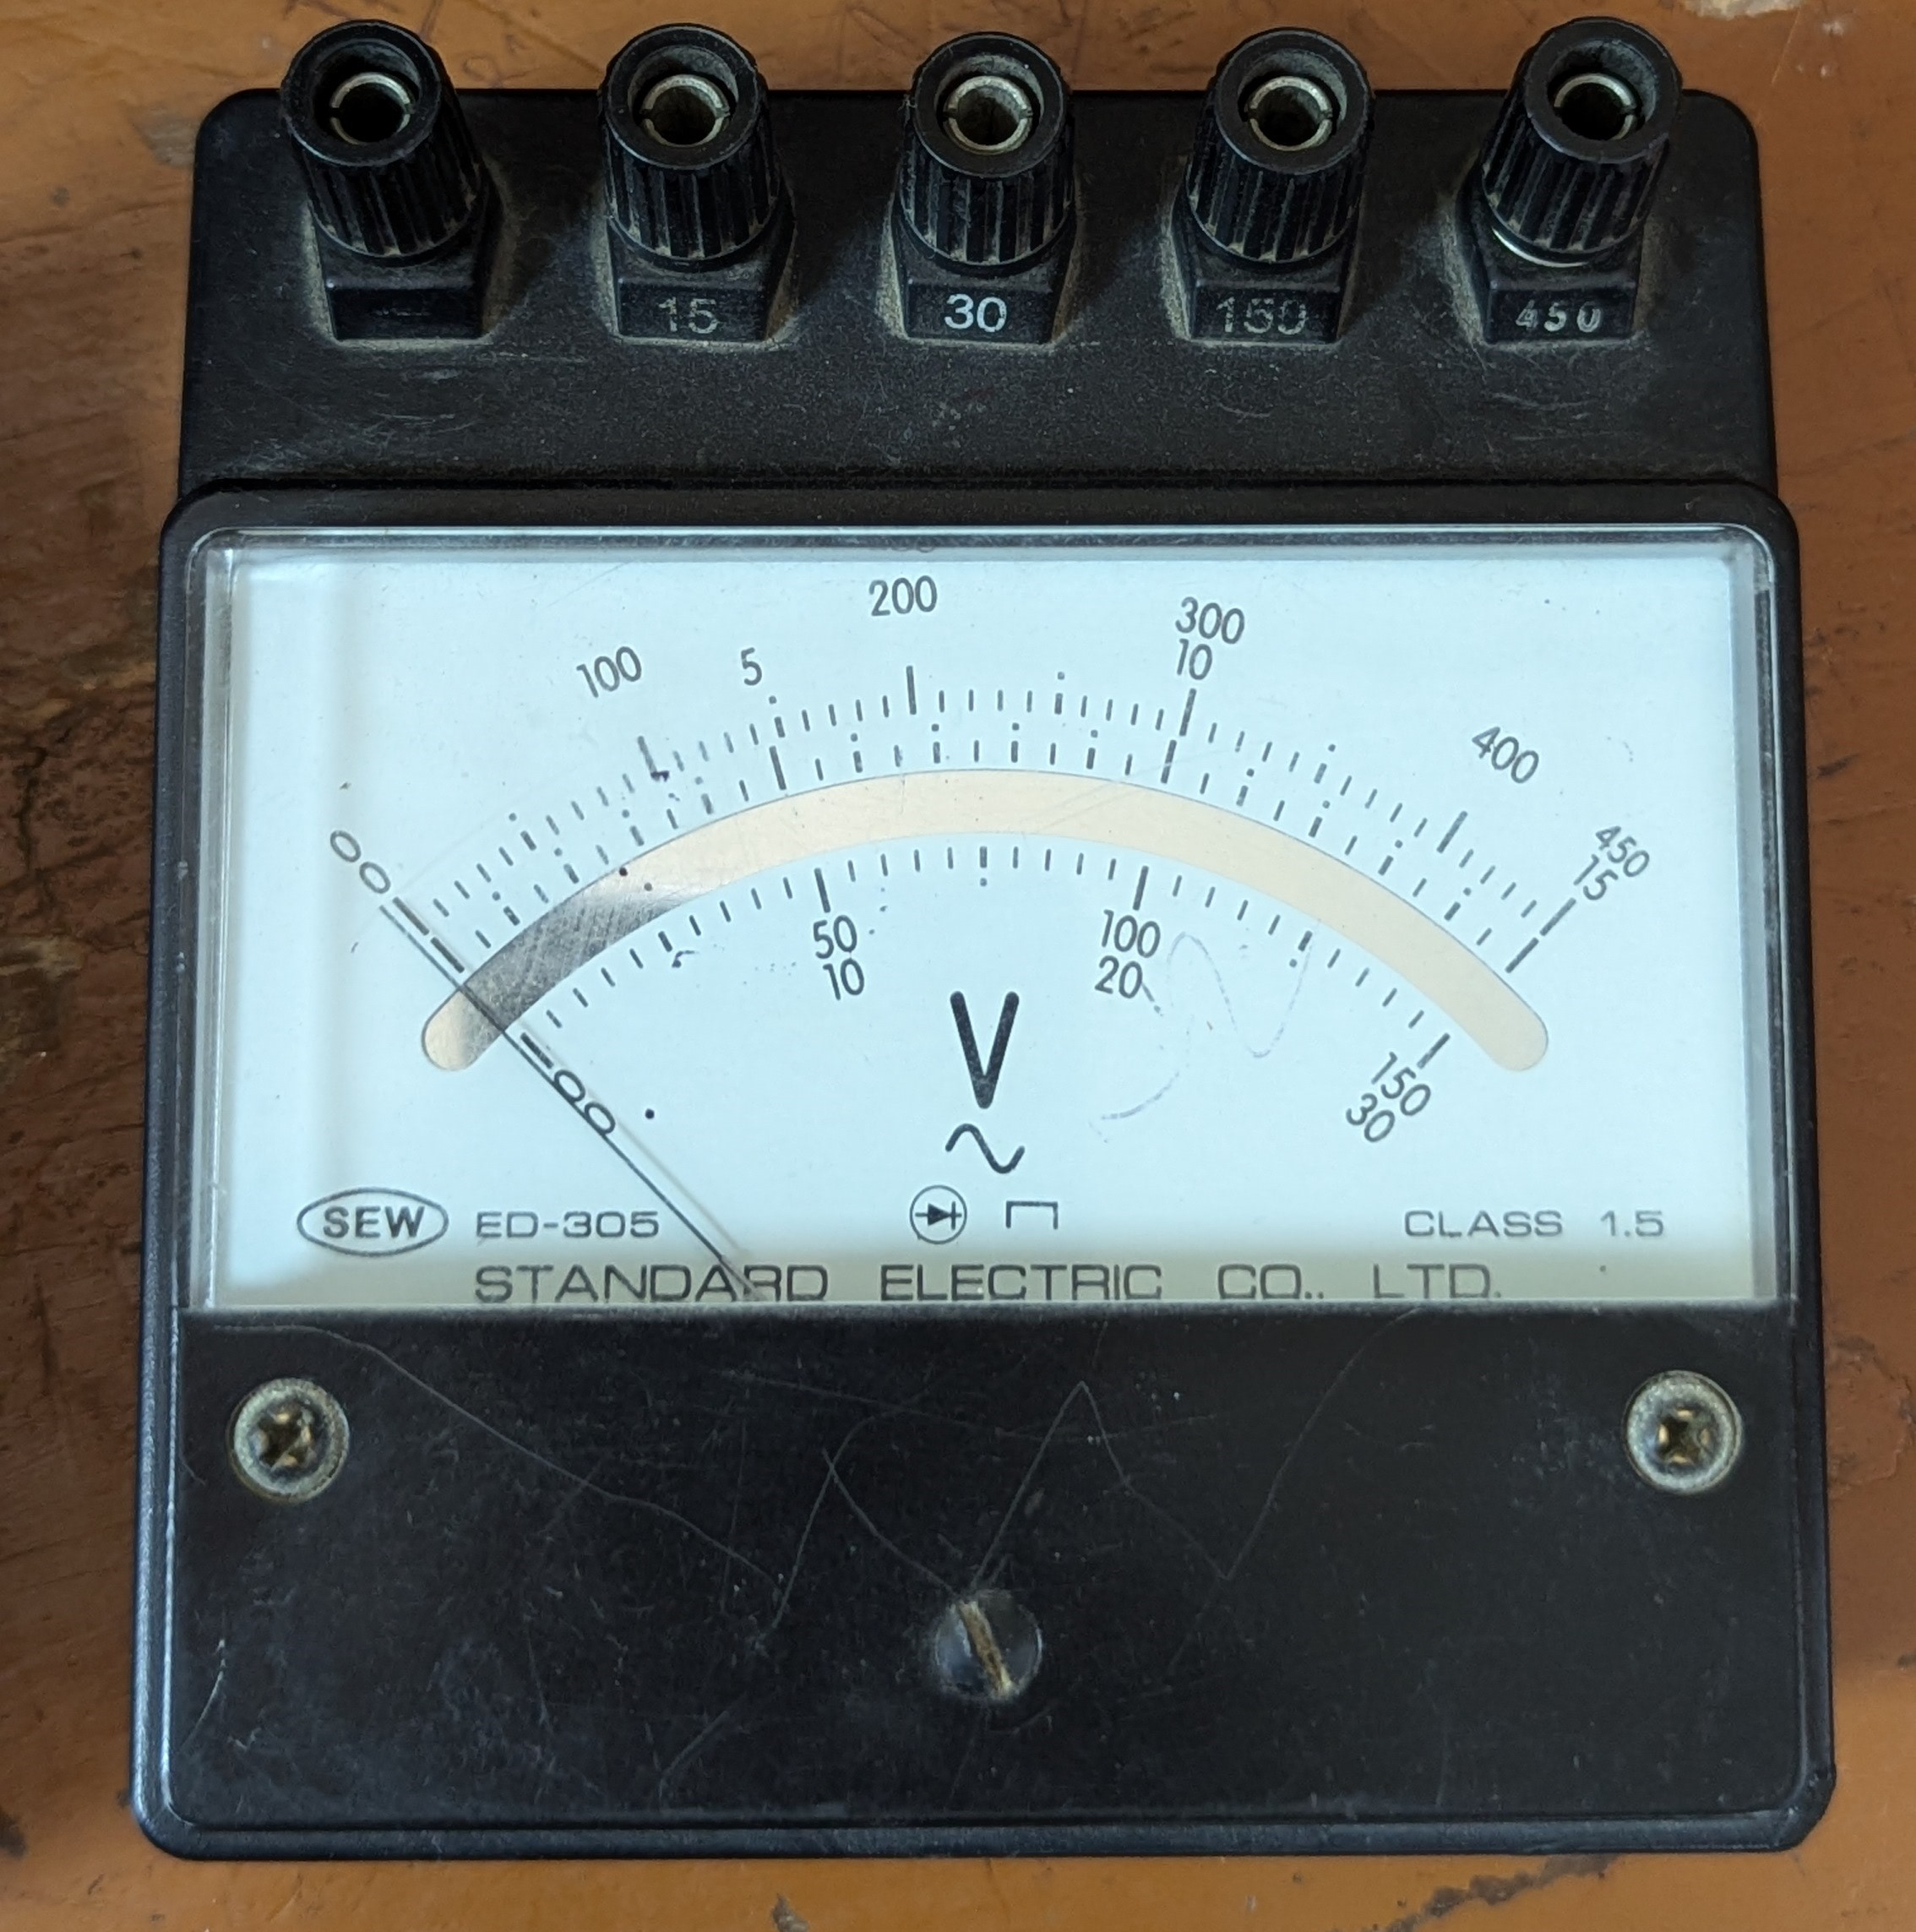
\includegraphics[width=0.42\linewidth]{Images/1}
	\caption{Voltmeter(AC)}
	\label{fig:1}
\end{figure}


	\subsection{Ammeter}
	An ammeter is an instrument used to measure the current flowing through a circuit. It is a vital tool for monitoring the flow of electrical current in both AC and DC circuits.
	
	\subsubsection{Types of Ammeter}
	\textbf{AC Ammeter:} Measures the current in alternating current (AC) circuits. It often uses a rectifier to convert the AC signal into a proportional DC signal before displaying the result. \\
	\textbf{DC Ammeter:} Measures the current in direct current (DC) circuits. It is designed to display the current flowing directly through a DC circuit.
	
	\subsubsection{Working Principle}
	Ammeters are connected in series with the circuit element to measure the current passing through it. The internal resistance of an ammeter is designed to be very low to avoid significant voltage drops or alteration in the circuit’s current during measurement.
	
\begin{figure}[H]
	\centering
	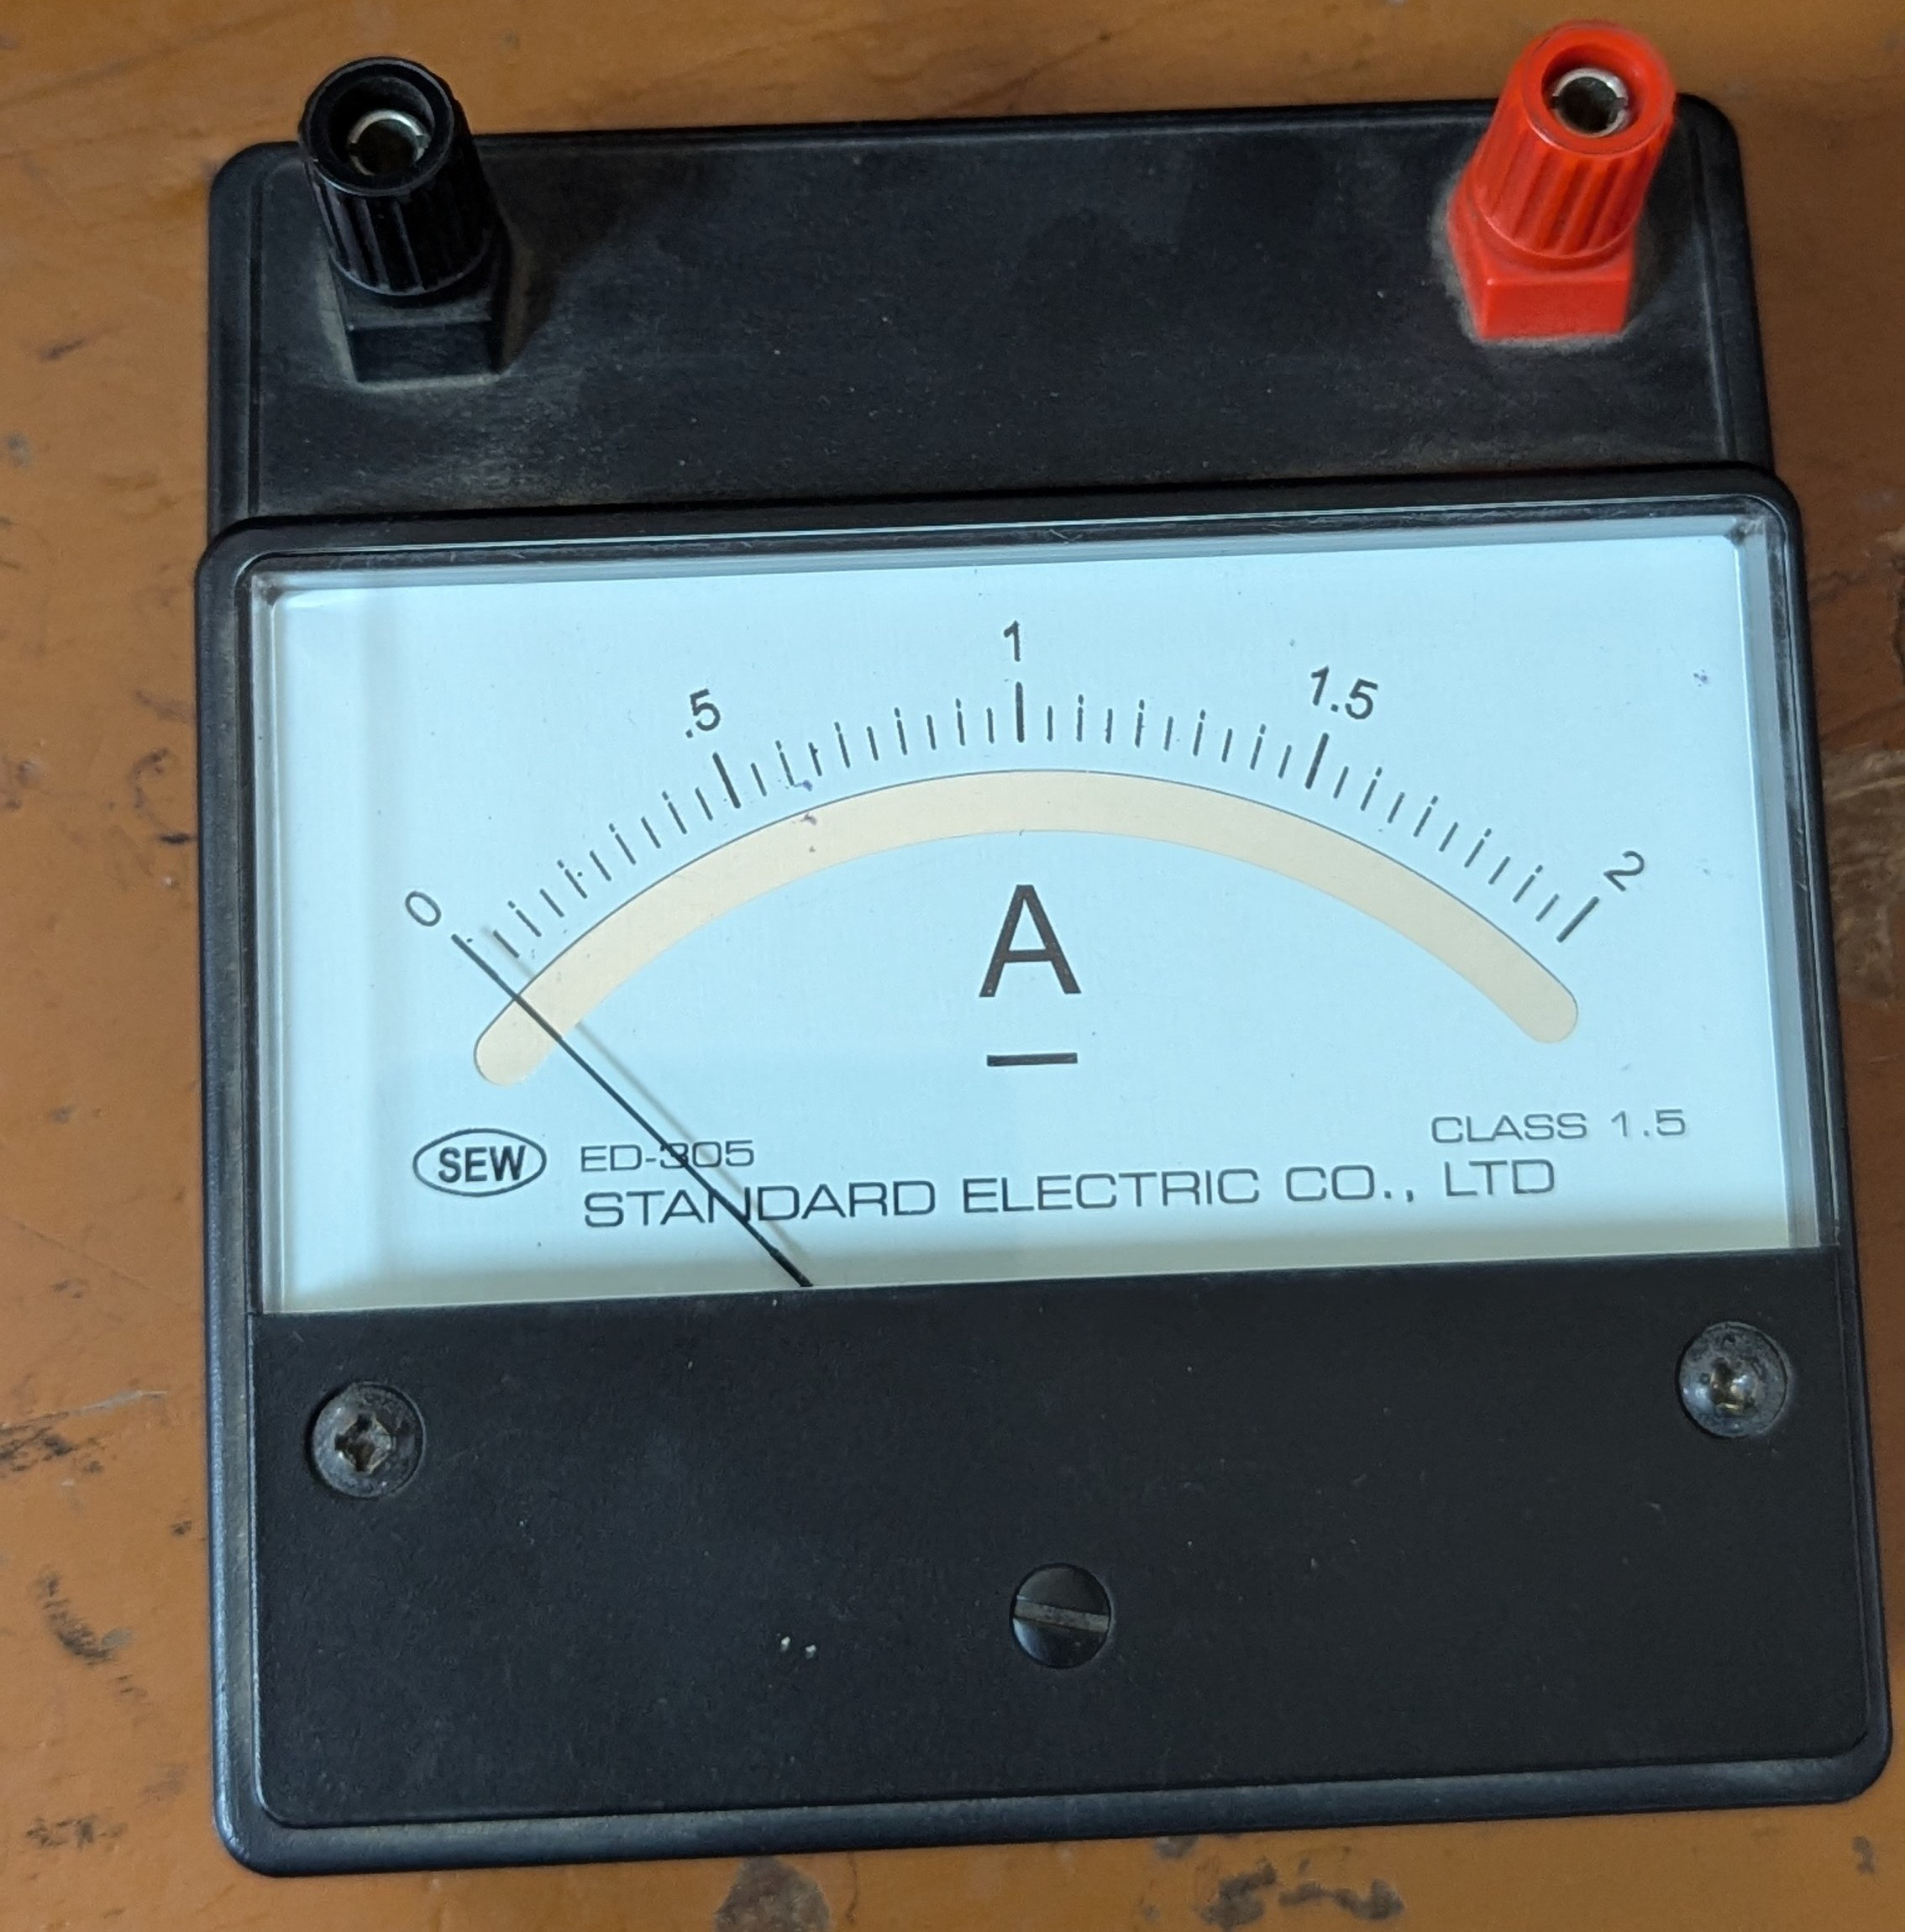
\includegraphics[width=0.42\linewidth]{Images/2}
	\caption{Ammeter(DC)}
	\label{fig:2}
\end{figure}
	
\subsection{Galvanometer}
A galvanometer is an instrument used to detect and measure small electric currents. It is highly sensitive and often used in laboratory settings for precise measurements of current.

\subsubsection{Types of Galvanometer}
\textbf{Moving Coil Galvanometer:} The most common type, it operates based on the interaction between the magnetic field and a current-carrying coil.\\
\textbf{Ballistic Galvanometer:} Specially designed to measure the quantity of charge that passes through the coil, used primarily in experiments involving transient currents.

\subsubsection{Working Principle}
A galvanometer works on the principle of electromagnetic deflection, where a current passing through a coil placed in a magnetic field produces a torque that deflects the coil. The deflection is proportional to the current, allowing precise measurement of small currents. The scale and pointer attached to the coil provide the current reading.

	
\begin{figure}[H]
	\centering
	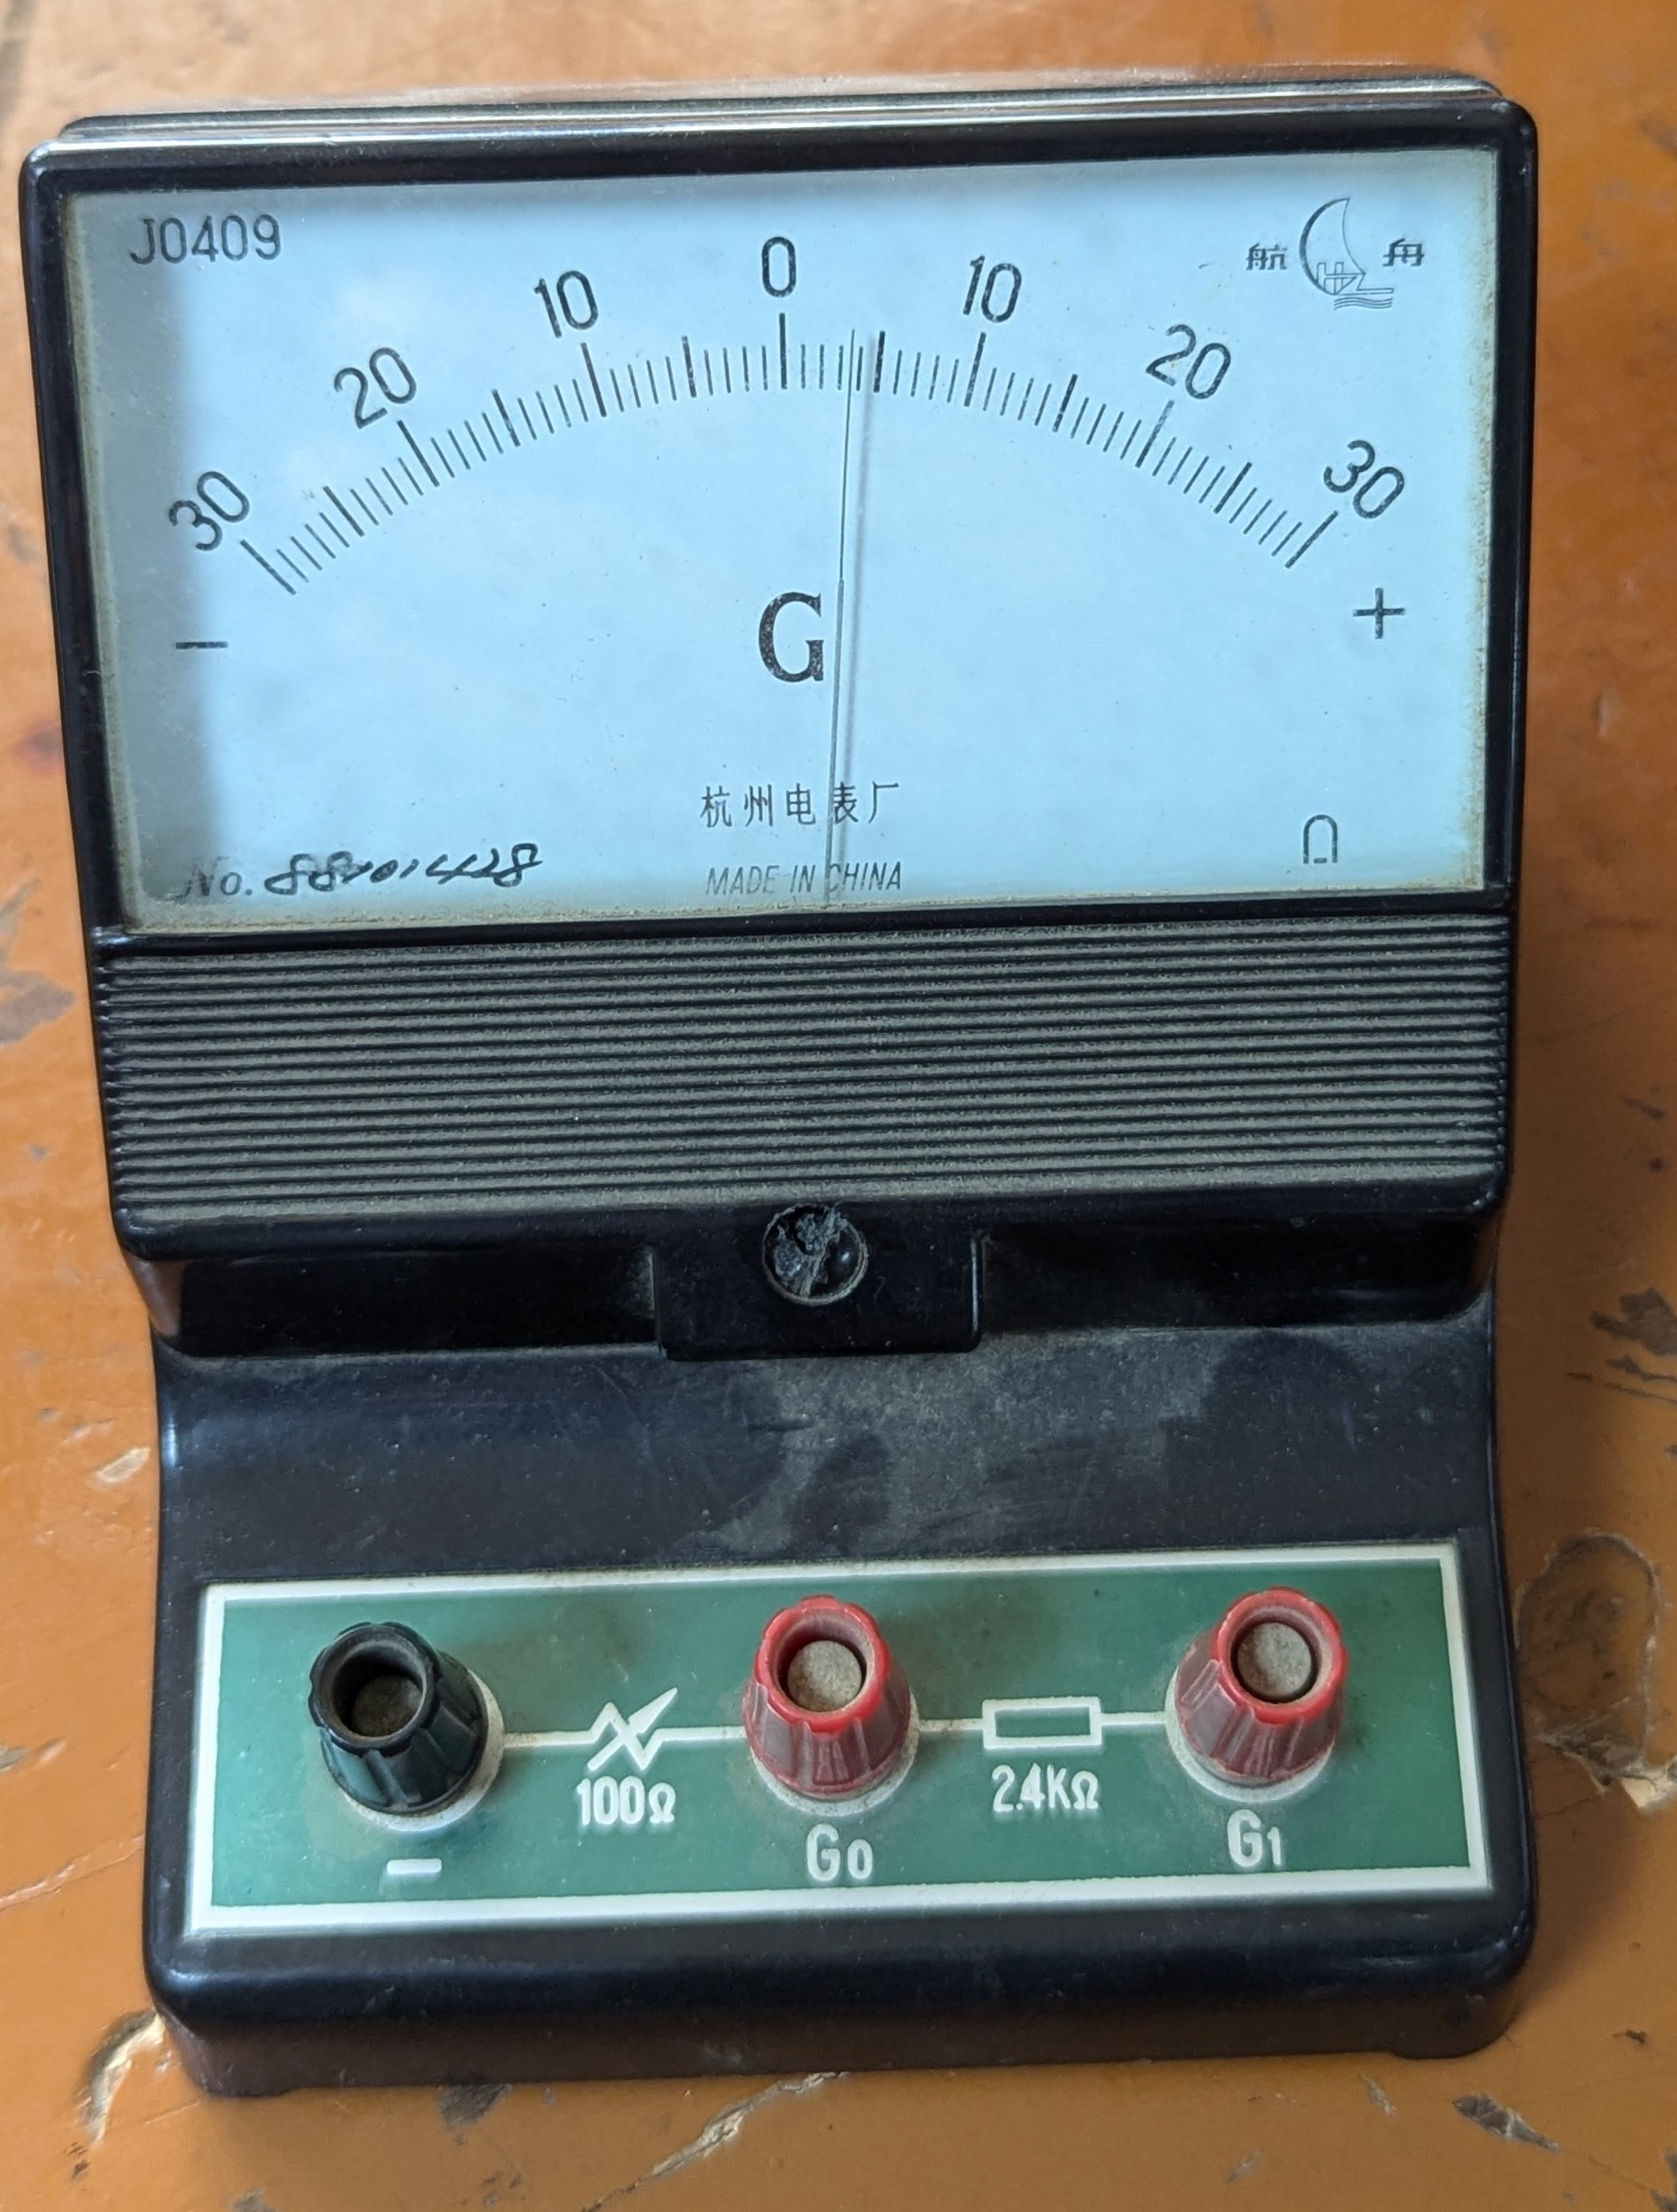
\includegraphics[width=0.45\linewidth, height=0.32 \textheight]{Images/3}
	\caption{Galvanometer}
	\label{fig:3}
\end{figure}

	\subsection{Resistors}
	Resistors are passive electrical components used to limit current and divide voltage in circuits. In the lab, resistors of specific values, such as 108$\Omega$, 37$\Omega$, and decade resistors, are commonly used for various experiments and measurements.
	
	\subsubsection{Types of Resistors in the Lab}
\textbf{108$\Omega$ and 37$\Omega$ Variable Resistors:} These are adjustable resistors where the resistance can be varied up to a maximum of 370$\Omega$ or 37$\Omega$, respectively. They are used in experiments where different resistance values are needed within these limits.\\
	
	
	\subsubsection{Working Principle}
	Resistors work by opposing the flow of electric current through the circuit. The resistance value, measured in ohms ($\Omega$), determines how much the current is reduced. Fixed resistors have a constant resistance value, while decade resistors allow adjustment to any desired value by selecting combinations of resistances.
	
	\subsubsection{Resistors with High Power Ratings}
	
	\begin{figure}[H]
		\centering
		\begin{subfigure}[t]{0.49\textwidth}
			\centering
				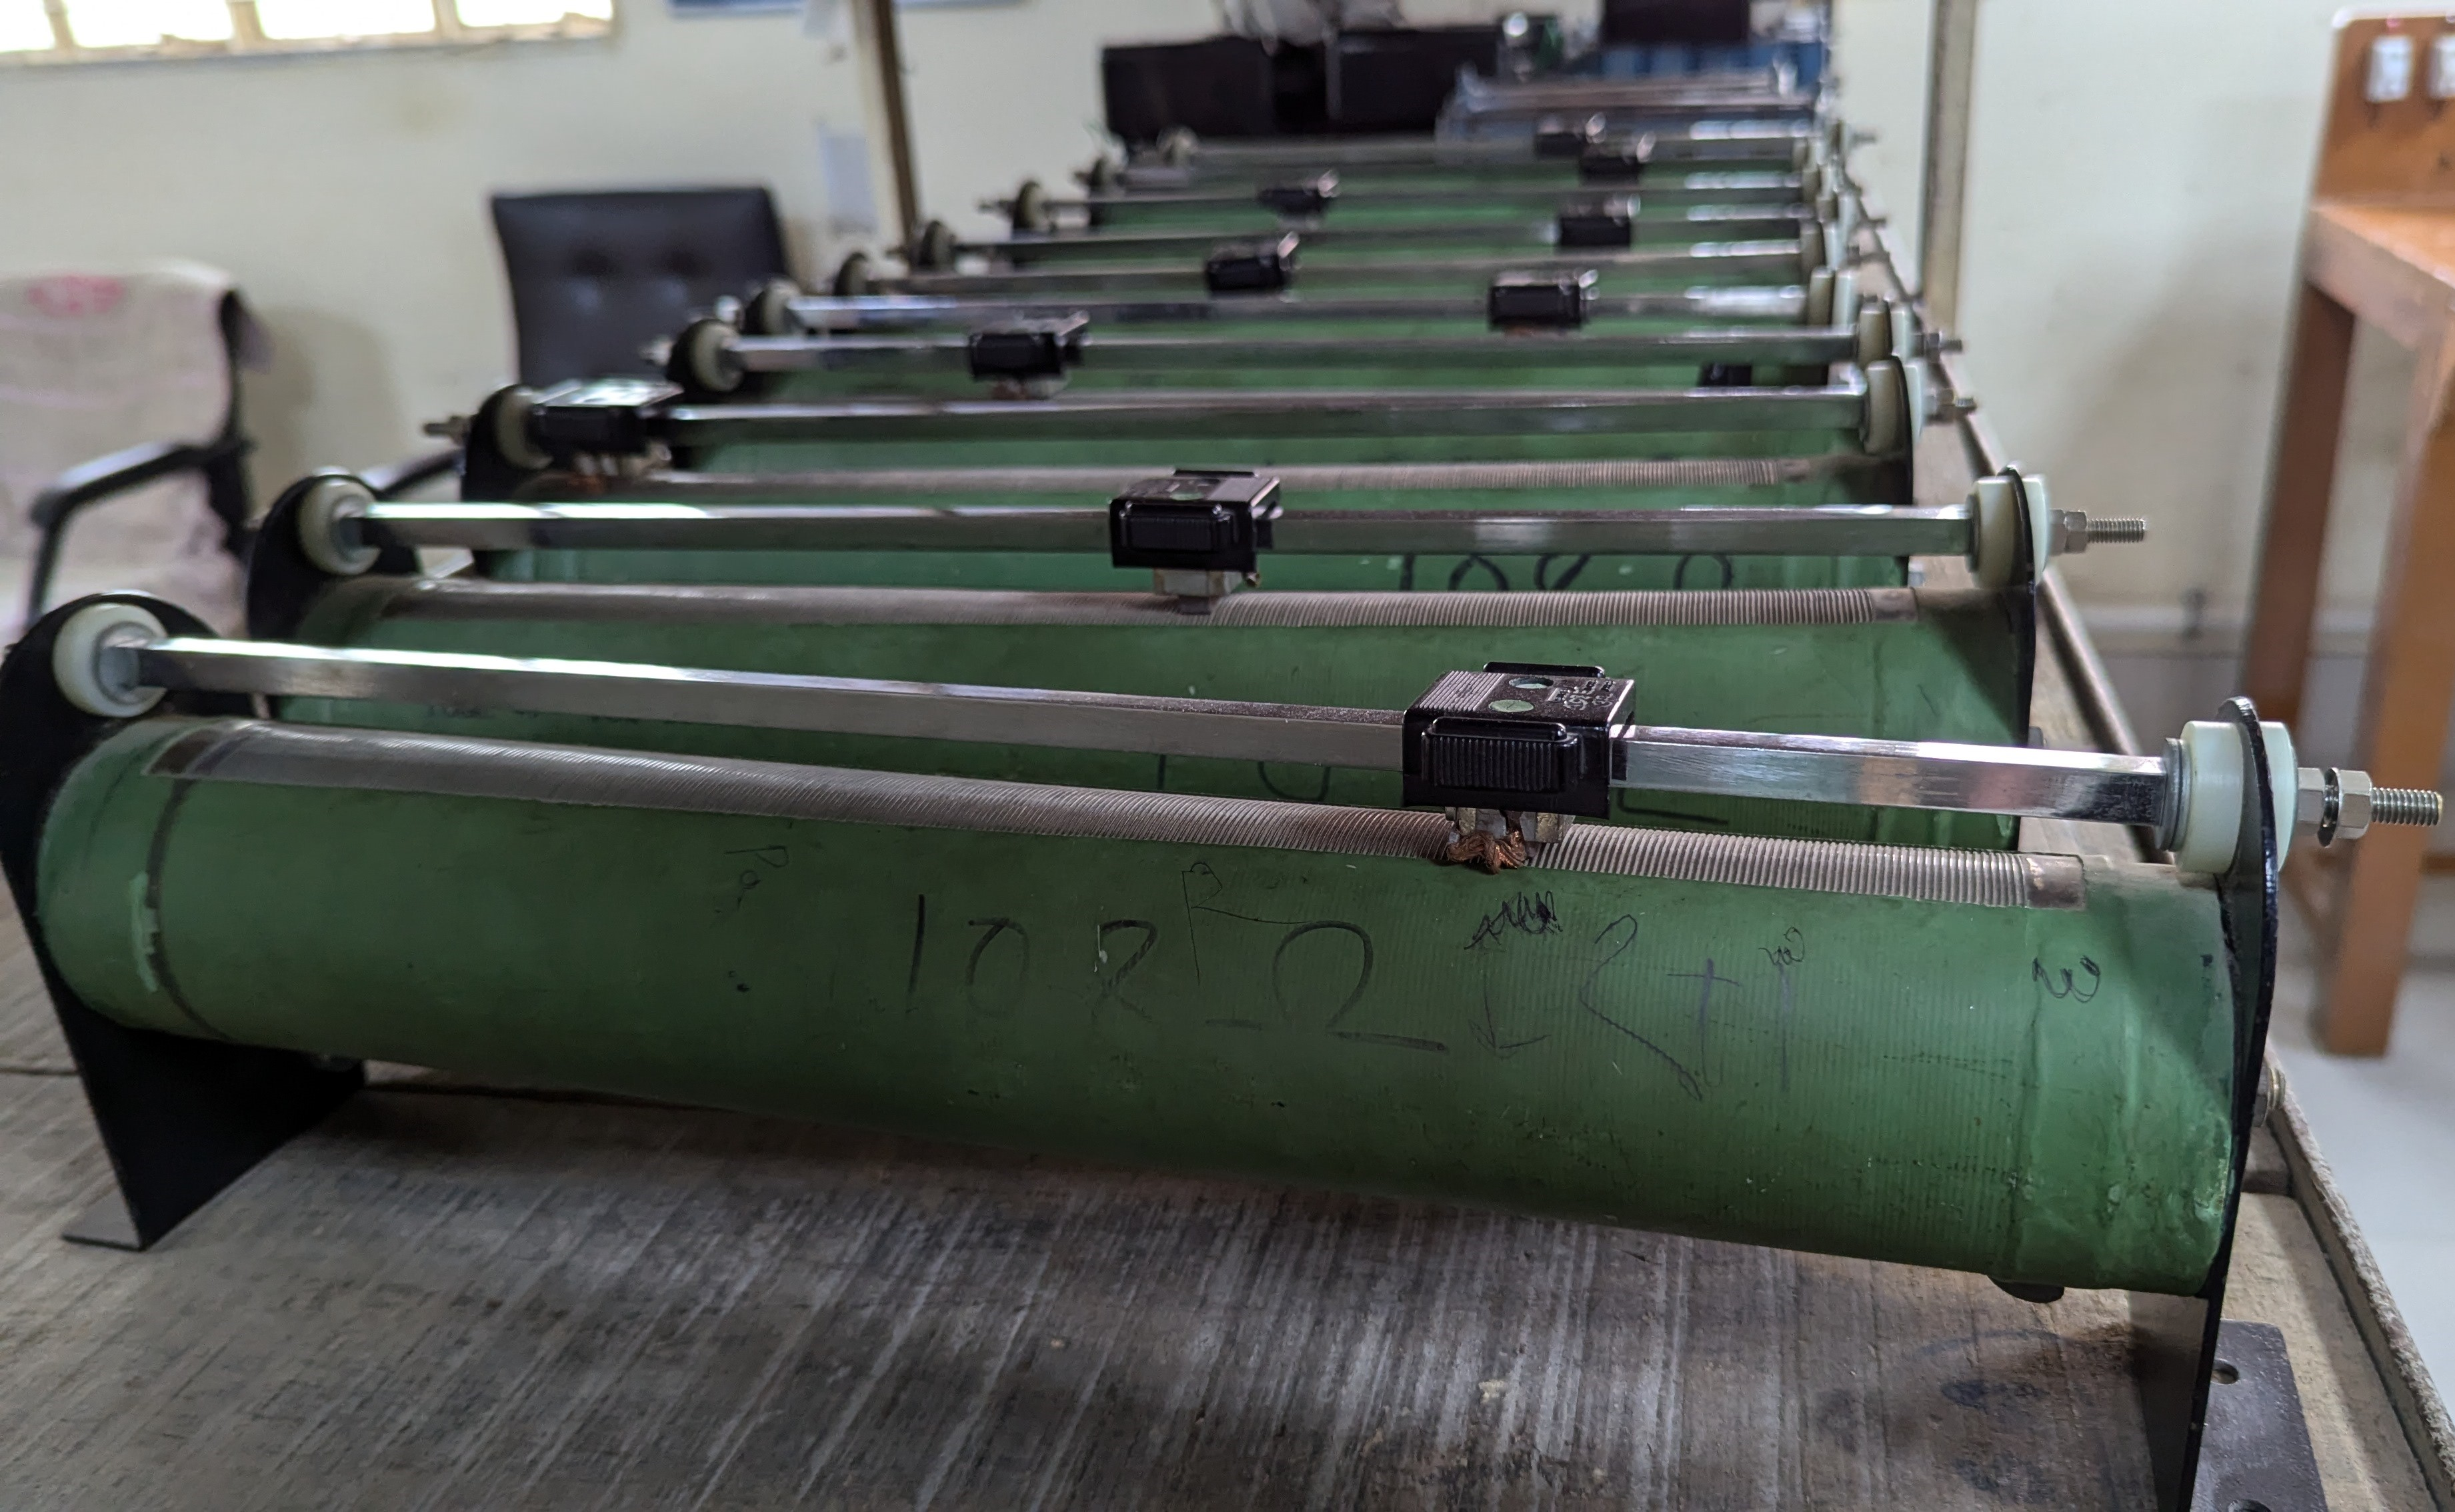
\includegraphics[width=1\linewidth]{Images/5}
			\caption{108$\Omega$}
		\end{subfigure}
		\hfill
		\begin{subfigure}[t]{0.49\textwidth}
			\centering
				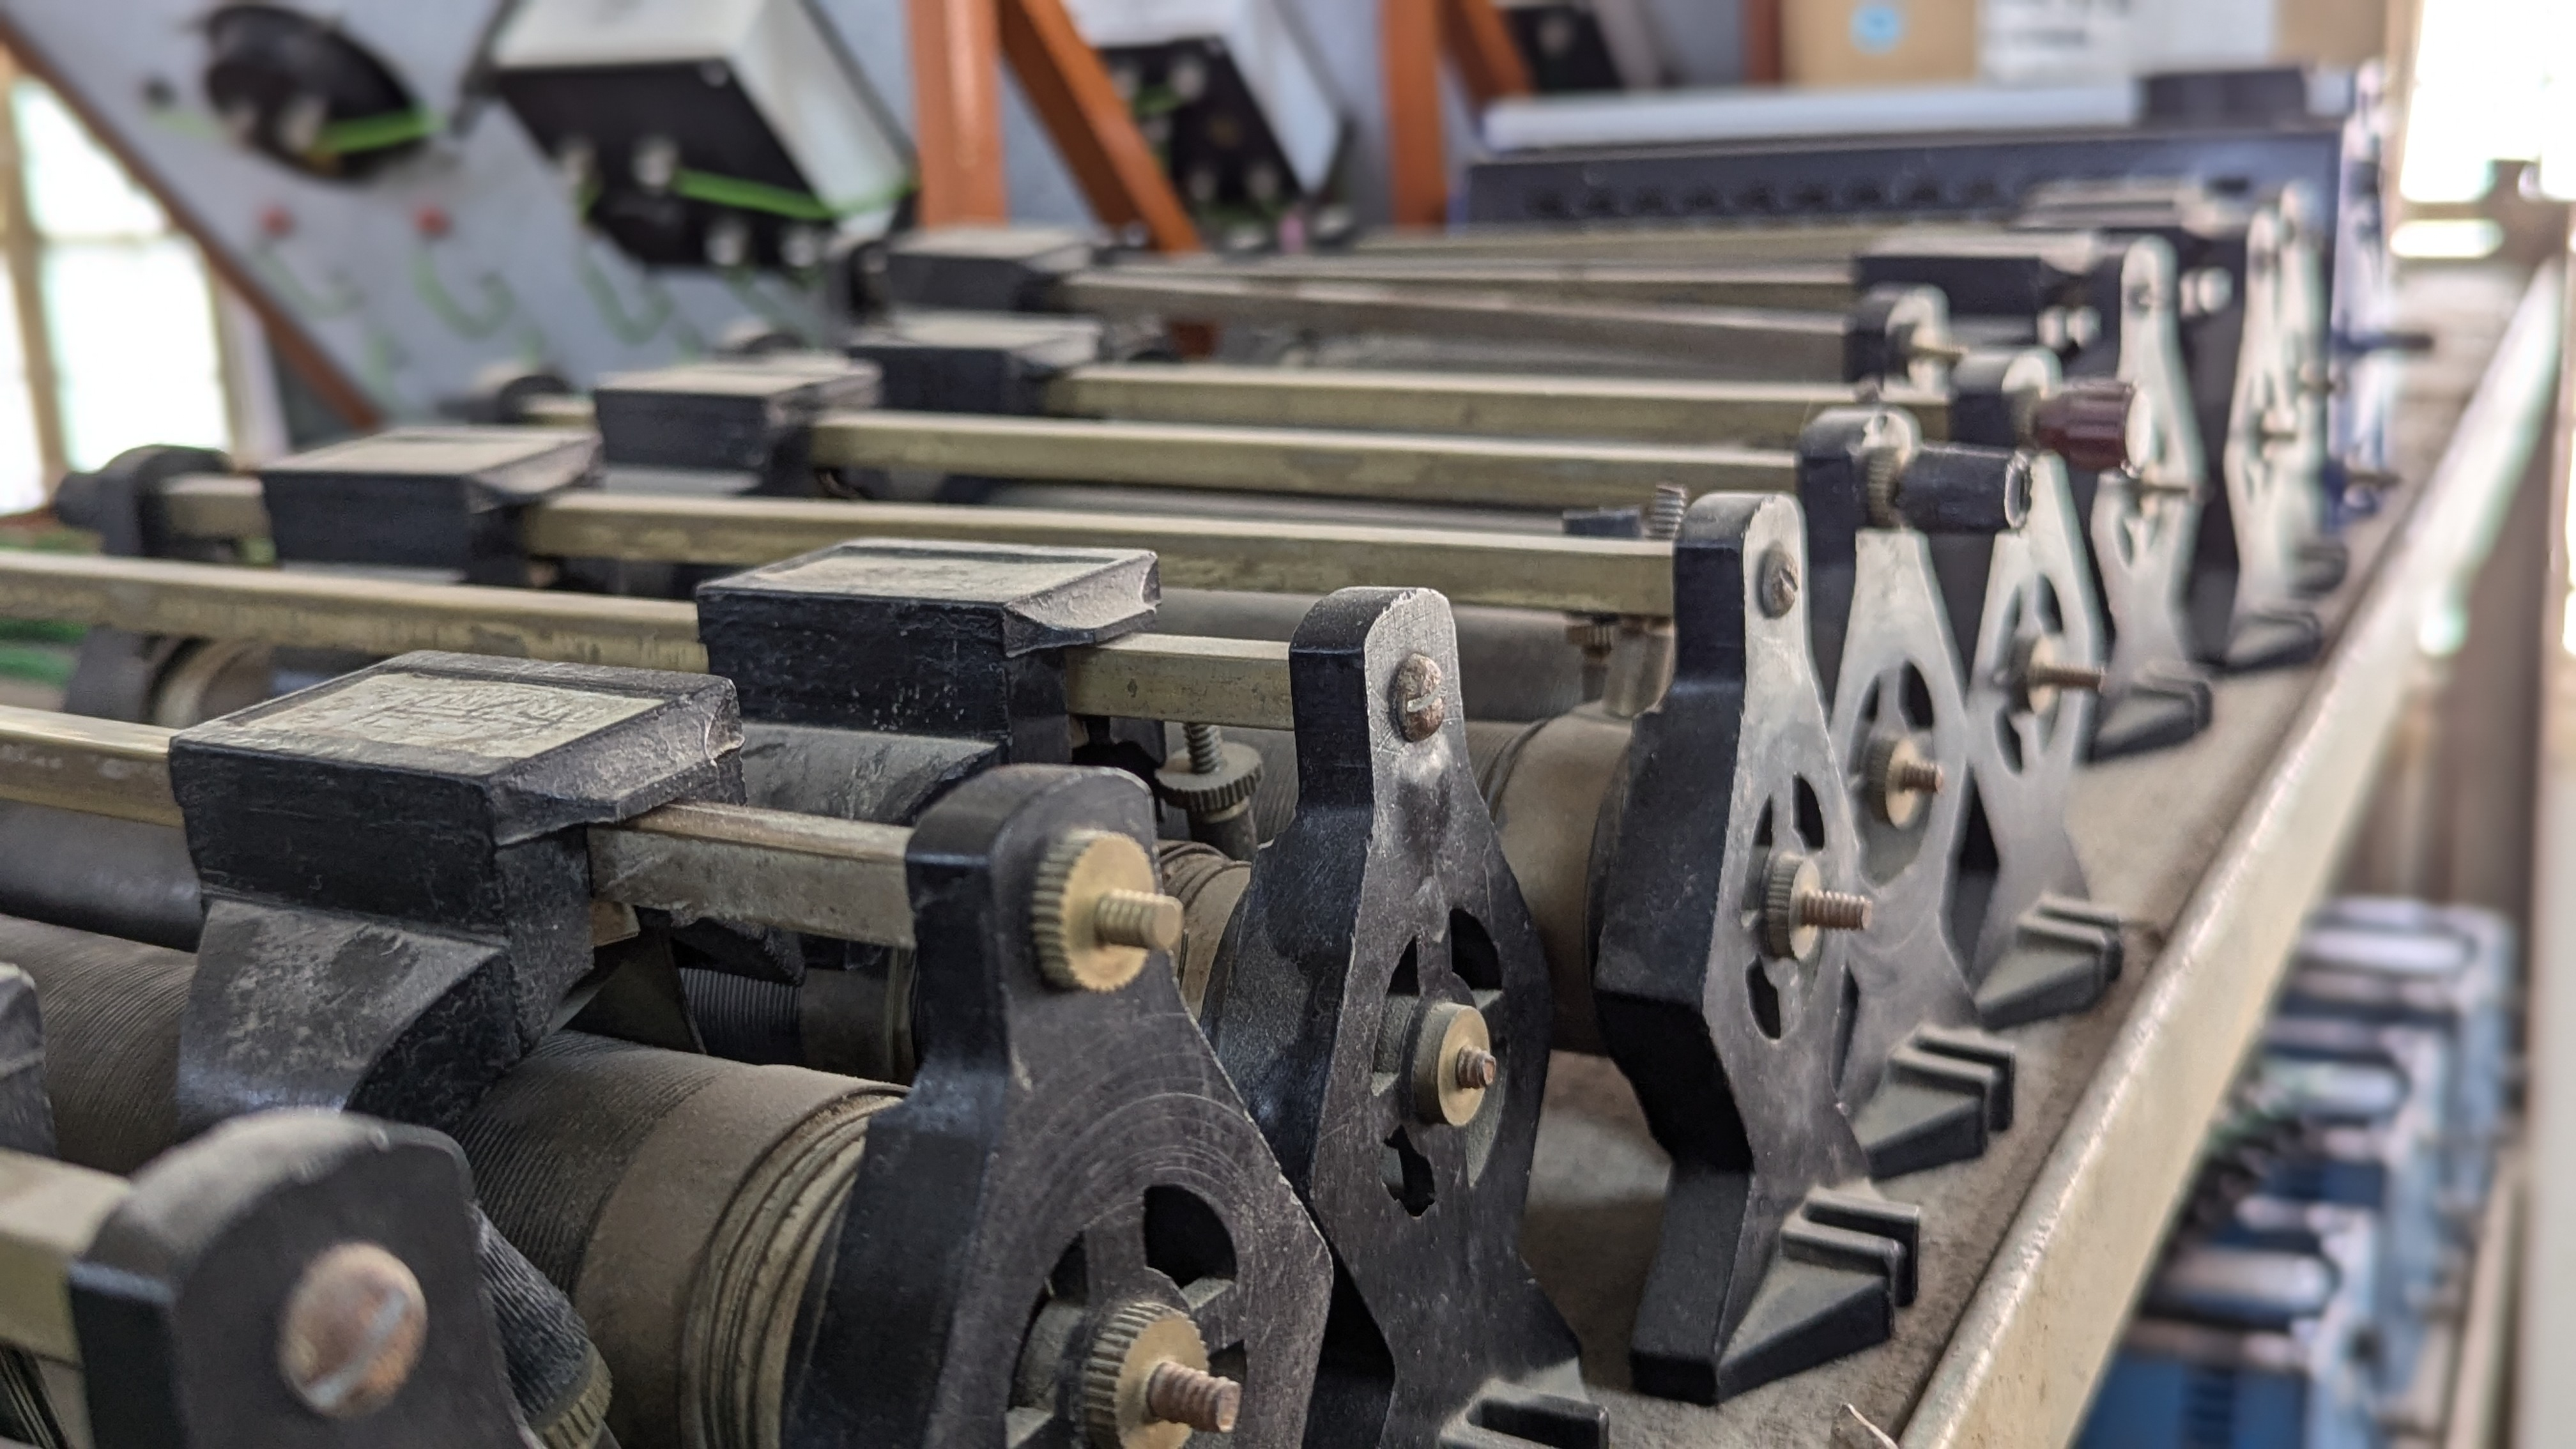
\includegraphics[width=1\linewidth]{Images/6}
			\caption{37$\Omega$}
		\end{subfigure}
	
		\begin{subfigure}[t]{0.49\textwidth}
			\centering
			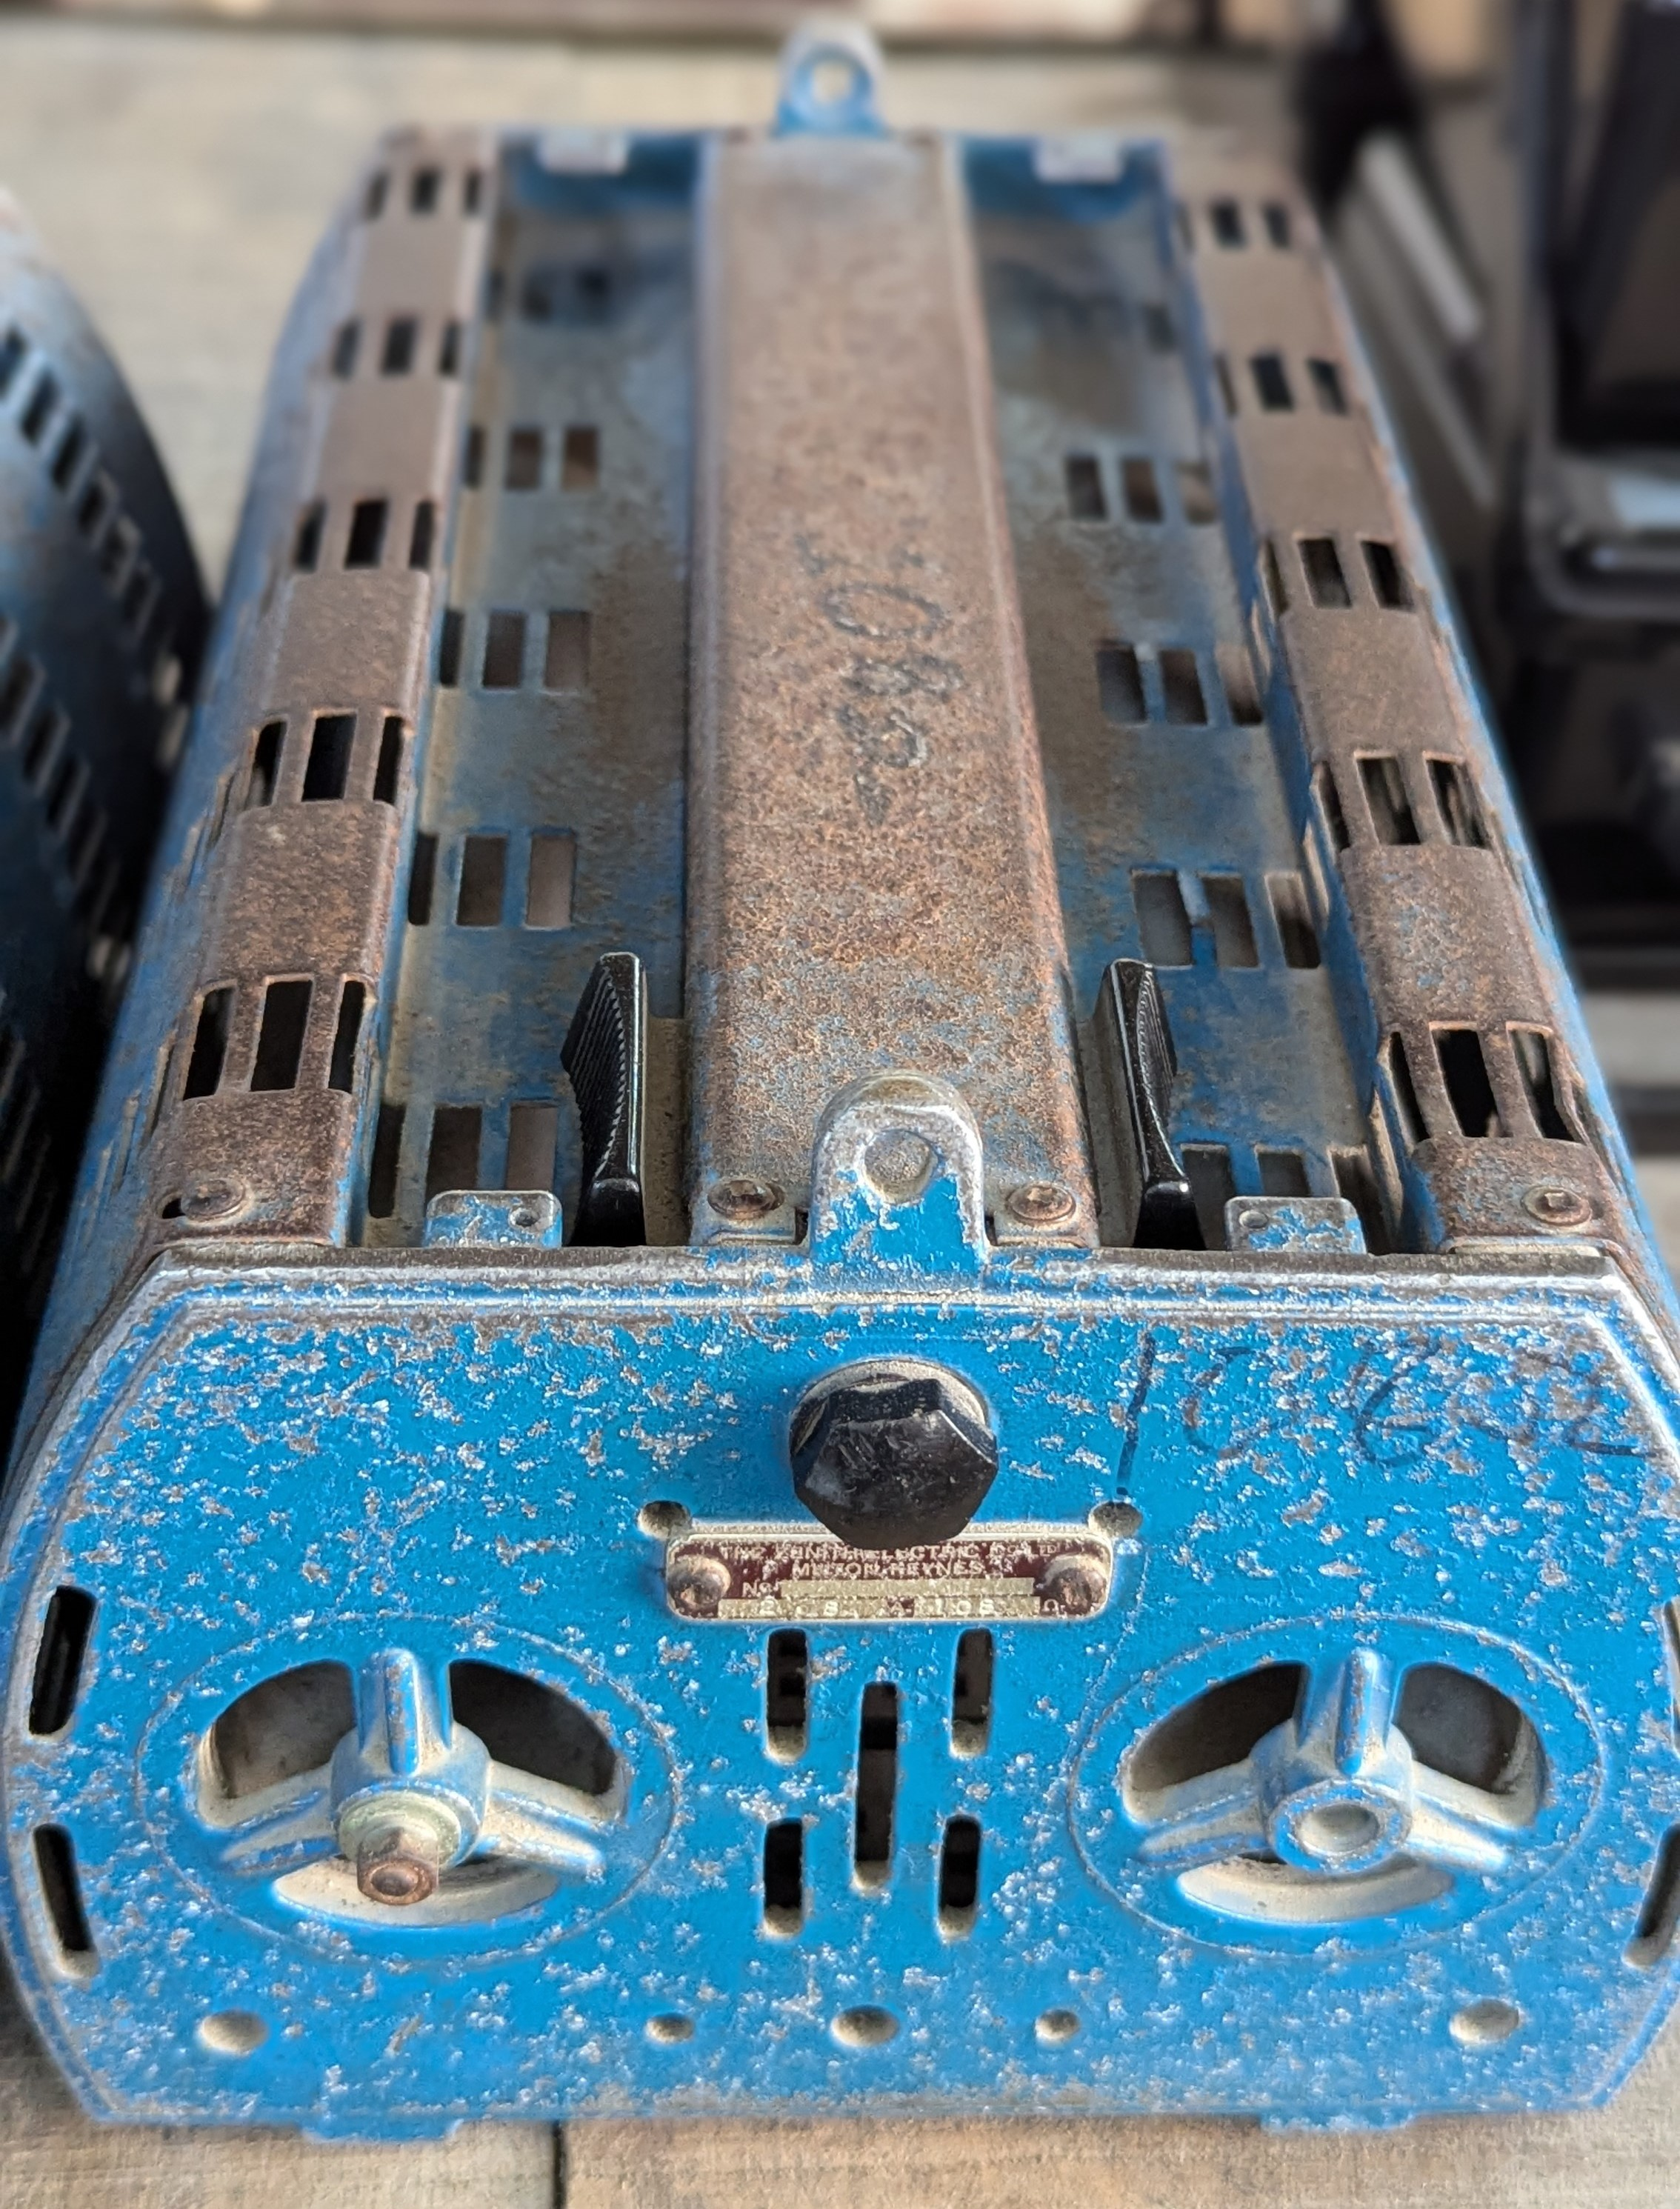
\includegraphics[angle=270, width=1\linewidth]{Images/7}
			\caption{108$\Omega$}
		\end{subfigure}
		\hfill
		\begin{subfigure}[t]{0.49\textwidth}
			\centering
			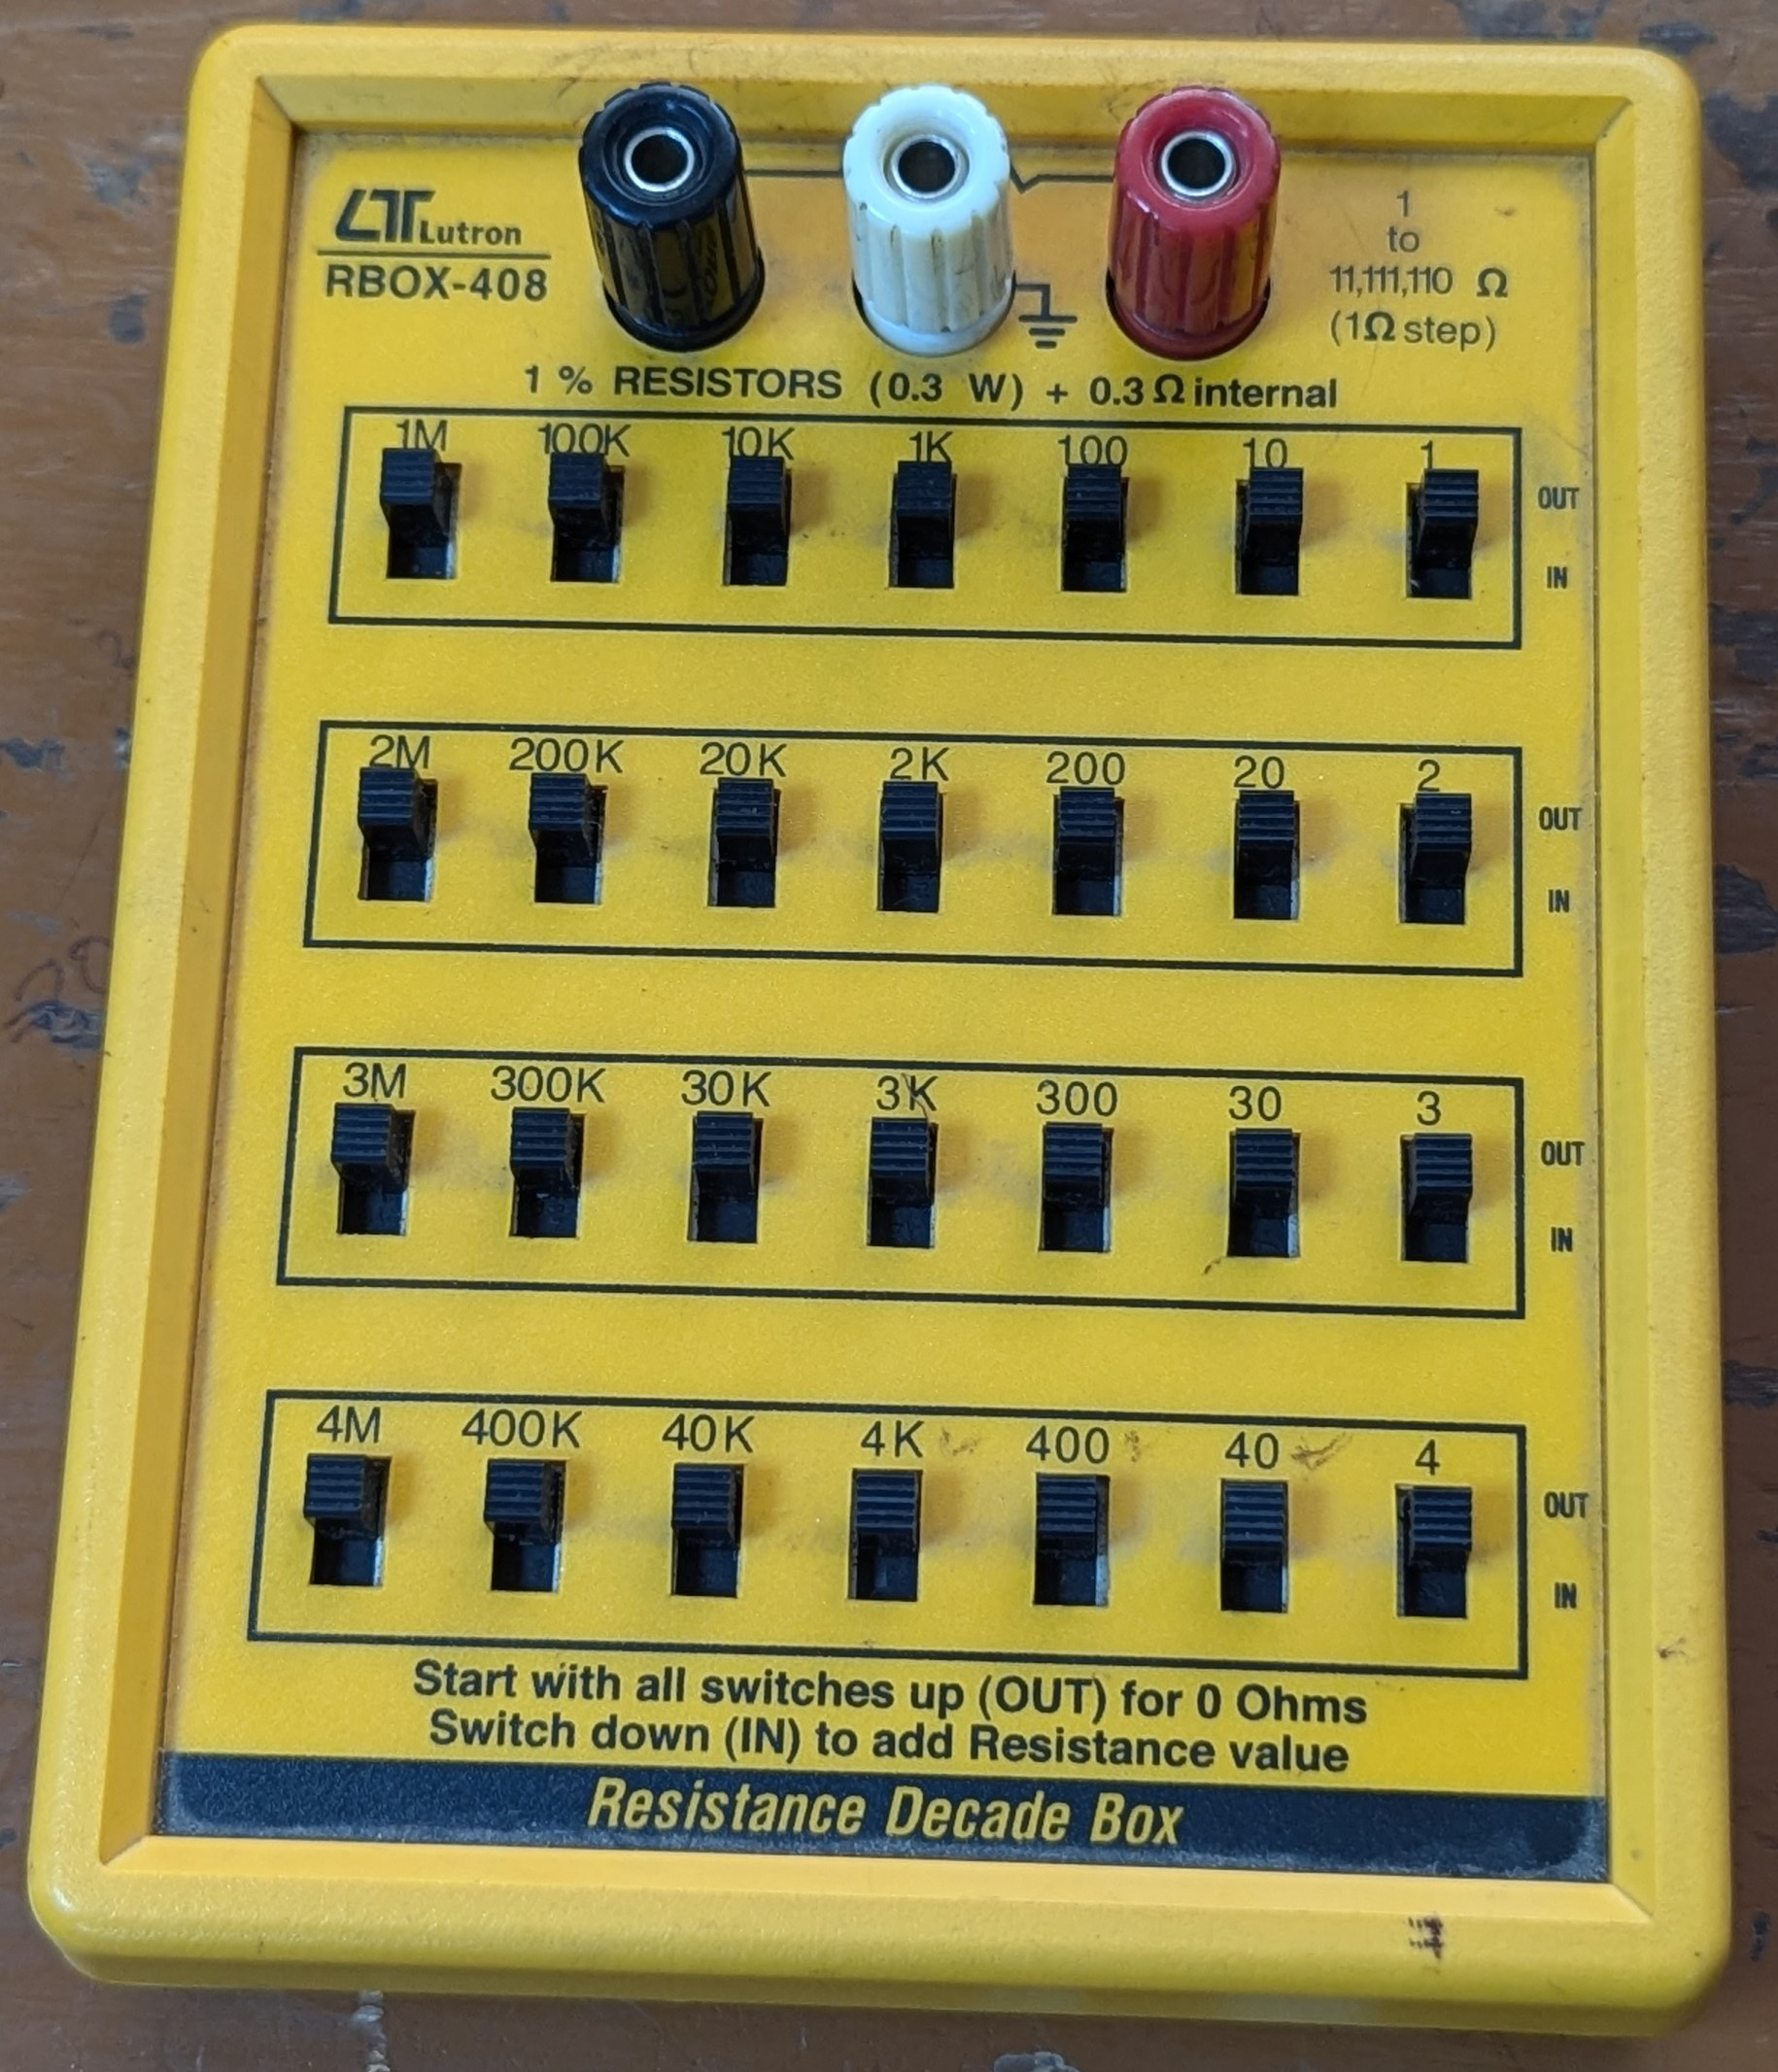
\includegraphics[angle=270, width=0.9\linewidth]{Images/8}
			\caption{Decade Resistor}
		\end{subfigure}
		
		\caption{Resistors }
		\label{fig:5}
	\end{figure}



	\subsubsection{Decade Resistor}
\textbf{Decade Resistor:} A decade resistor is a precision instrument used to provide a selectable resistance value. It
consists of multiple resistors arranged in decades (powers of ten), allowing users to dial in
a desired resistance by adjusting switches. Each switch represents a specific range, such as
1$\Omega$, 10$\Omega$, 100$\Omega$ etc. It allows precise selection of resistance values for testing and calibration
in circuits. Resistance can be adjusted in steps, making it highly flexible for experimental
setups. It is used in circuit design, testing, calibration, and educational labs for simulating
different resistance loads. Decade resistors provide stable, accurate resistance values, making
them essential for fine-tuning and precise measurements in electrical experiments.


\subsection{Inductor}
An inductor is a passive electrical component that stores energy in the form of a magnetic field when current flows through it. It consists of a coil of wire, and its key property is inductance, measured in henries (H), which represents the inductor’s ability to oppose changes in current. Inductors are commonly used in filters, transformers, energy storage in power supplies, and tuning circuits.\\
The inductor available in our measurement lab has a rating of 24 $\mu$H.

	
	\begin{figure}[H]
		\centering
		\begin{subfigure}[t]{0.49\textwidth}
			\centering
			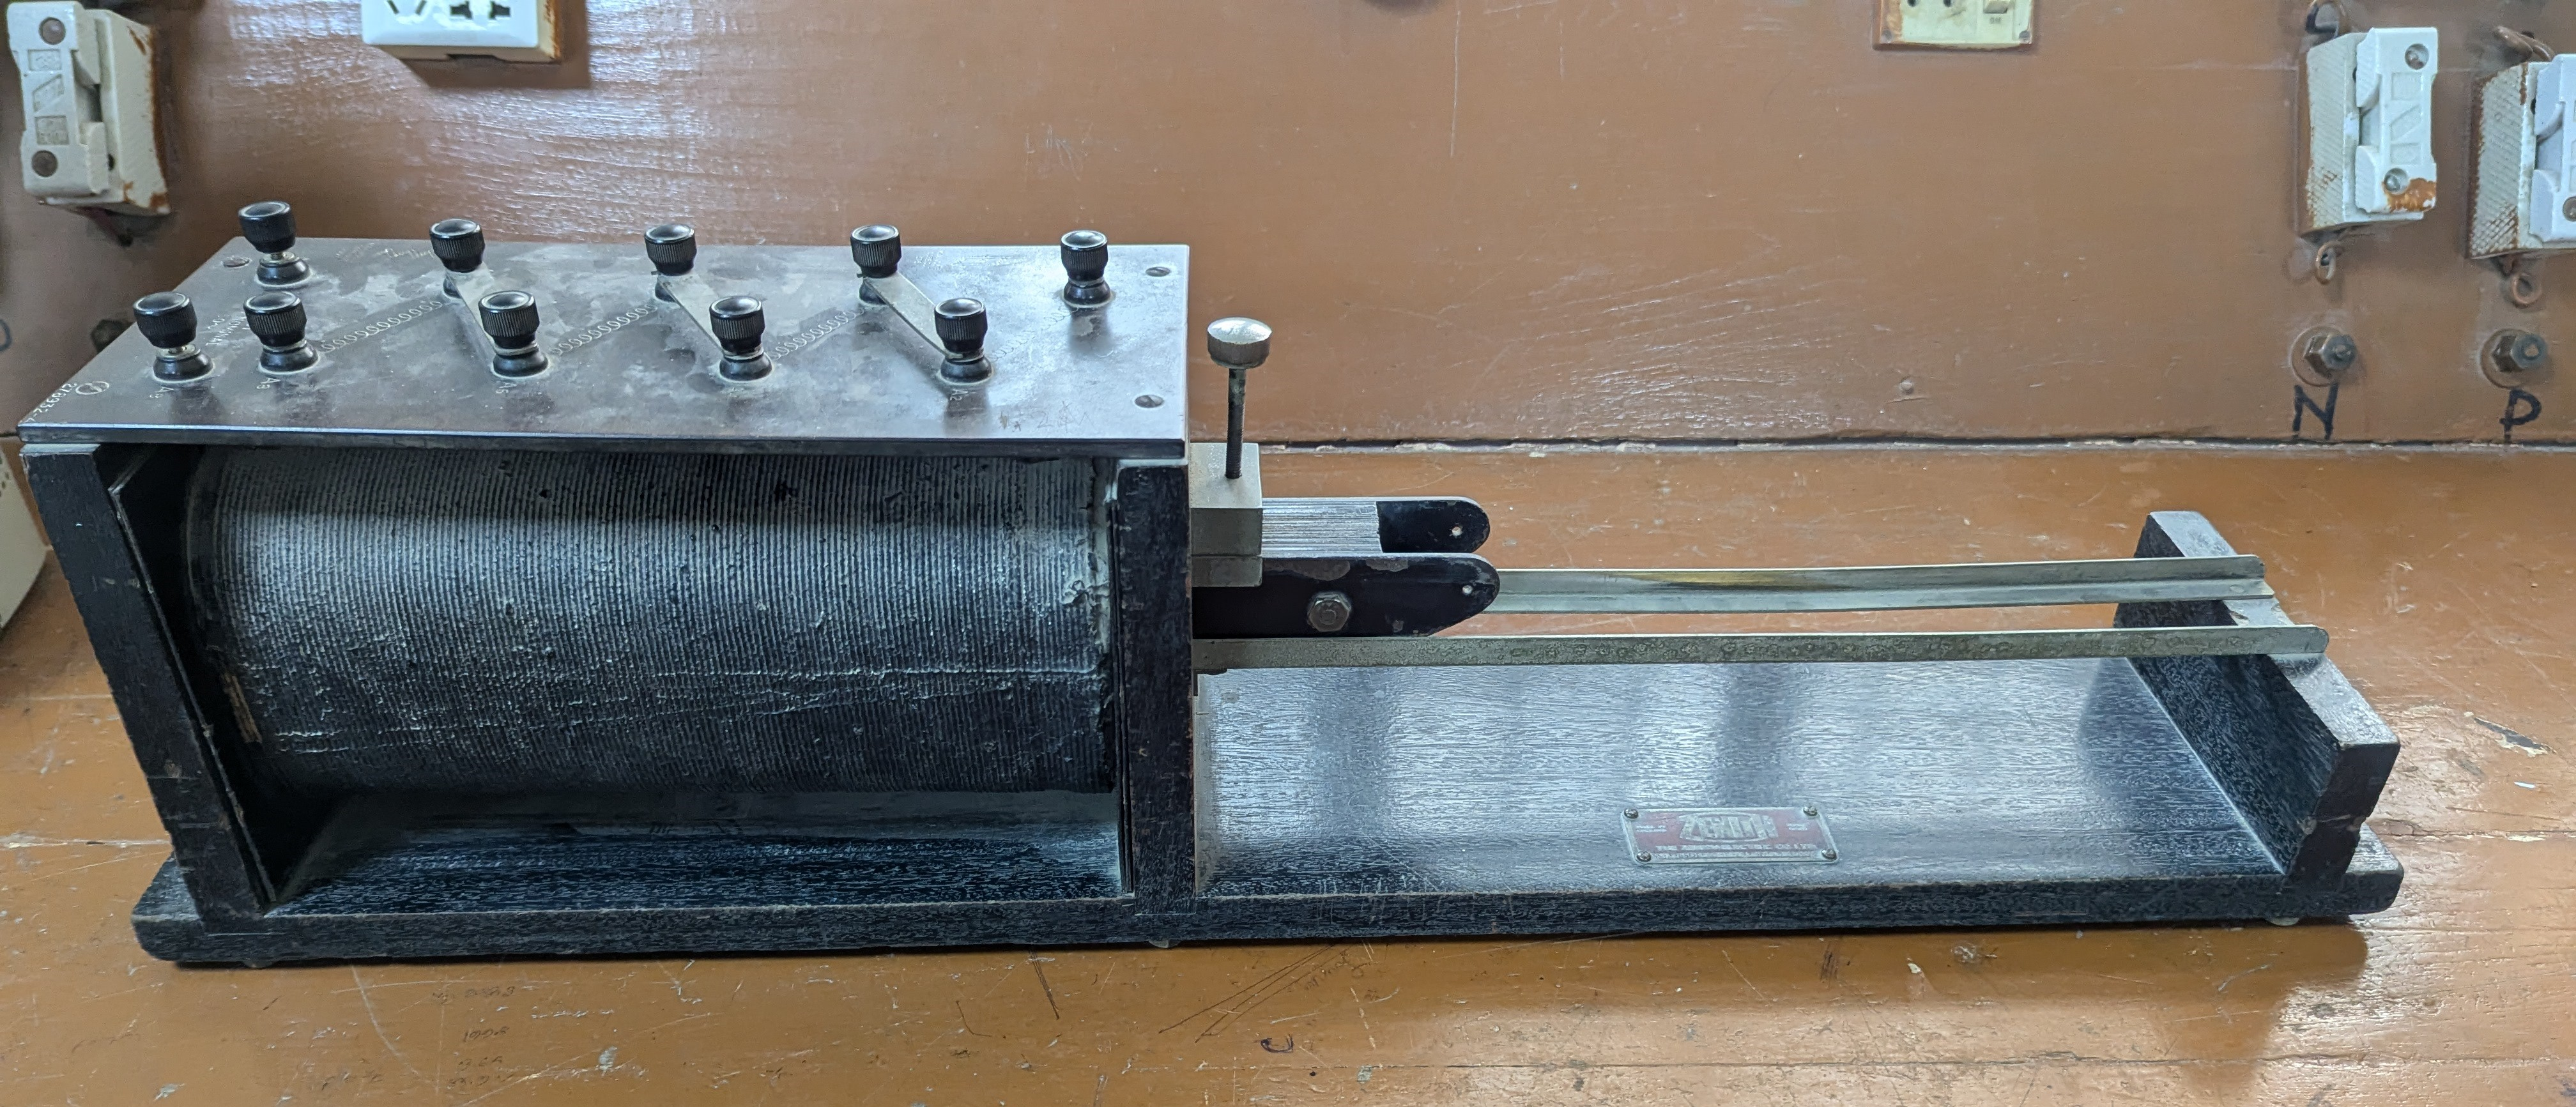
\includegraphics[width=1\linewidth]{Images/10}
			\caption{Side View}
		\end{subfigure}
		\hfill
		\begin{subfigure}[t]{0.49\textwidth}
			\centering
			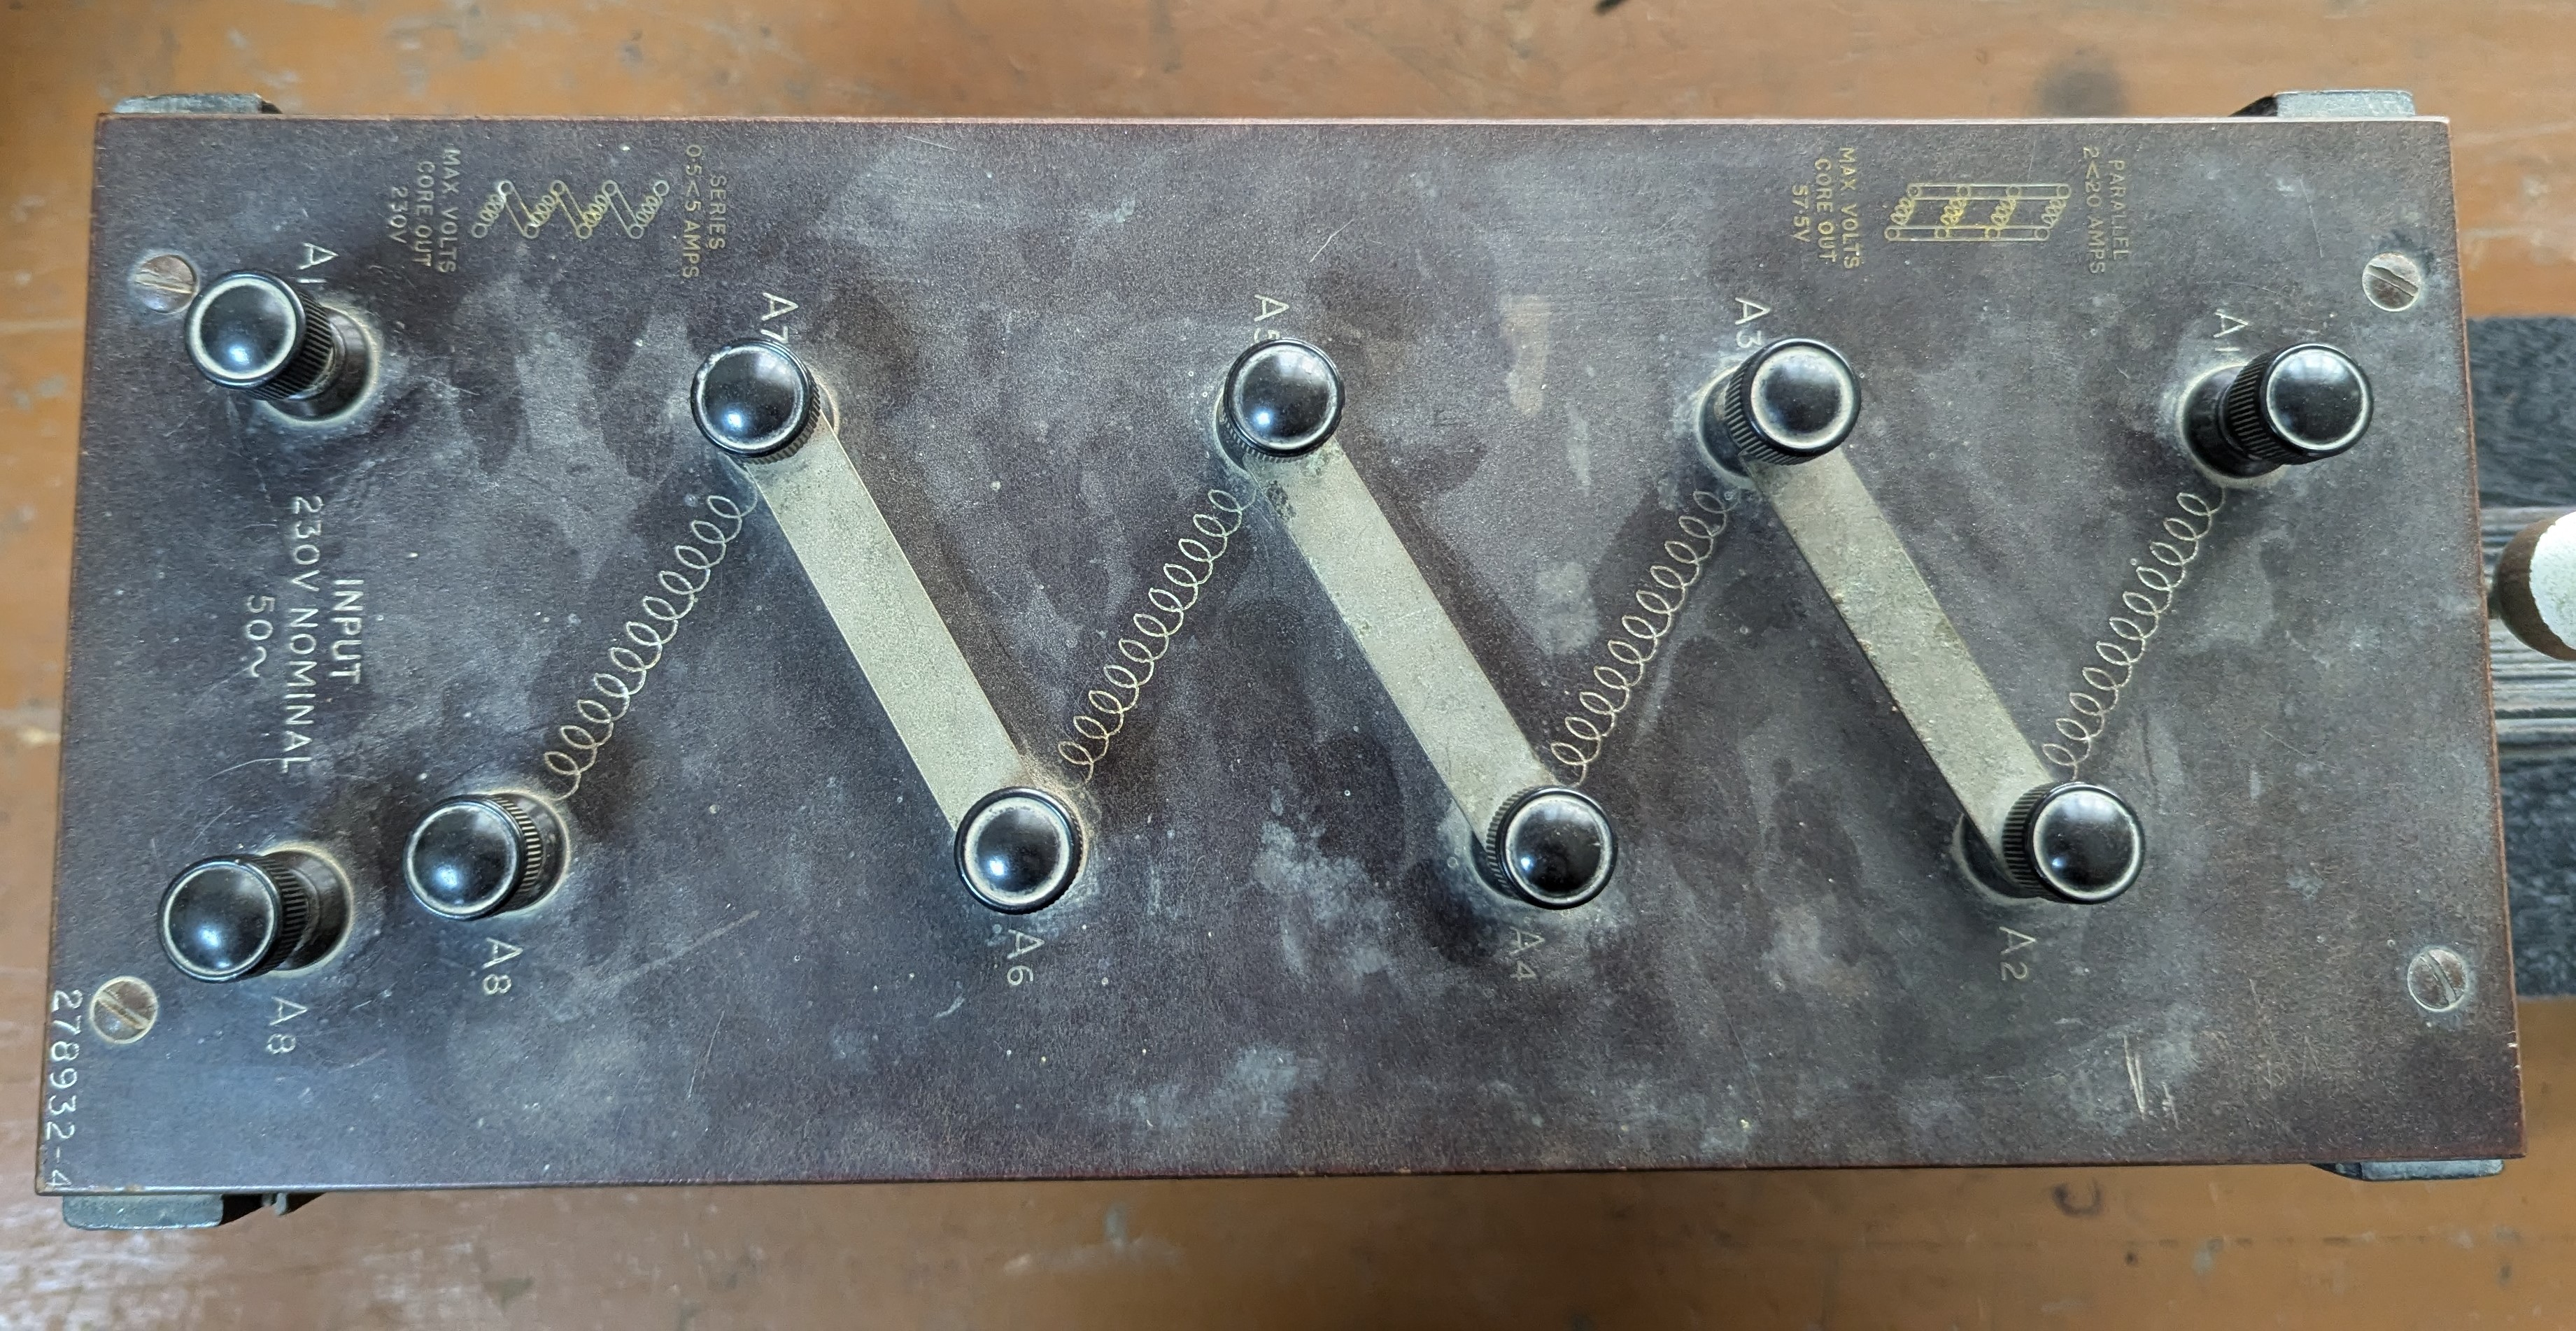
\includegraphics[width=1\linewidth]{Images/11}
			\caption{Top View}
		\end{subfigure}
	
		\caption{Inductor }
		\label{fig:5}
	\end{figure}
	
	
\subsection{Capacitor}
A capacitor is a passive component that stores energy as an electric field between two conductive plates separated by a dielectric. When voltage is applied, it stores electrical energy.\\
	 \textbf{Polarized Capacitors:} Have specific positive and negative terminals (e.g., electrolytic capacitors), used for larger capacitance values.\\
	 \textbf{Non-Polarized Capacitors:} Can be connected in any direction (e.g., ceramic capacitors), used in high-frequency applications.\\
 In our lab, capacitors with ratings from 16 mF to 128 mF are available, indicating their charge storage capacity.

	
	\begin{figure}[H]
		\centering
		\scalebox{.95}{
		\begin{subfigure}[t]{0.32\textwidth}
			\centering
			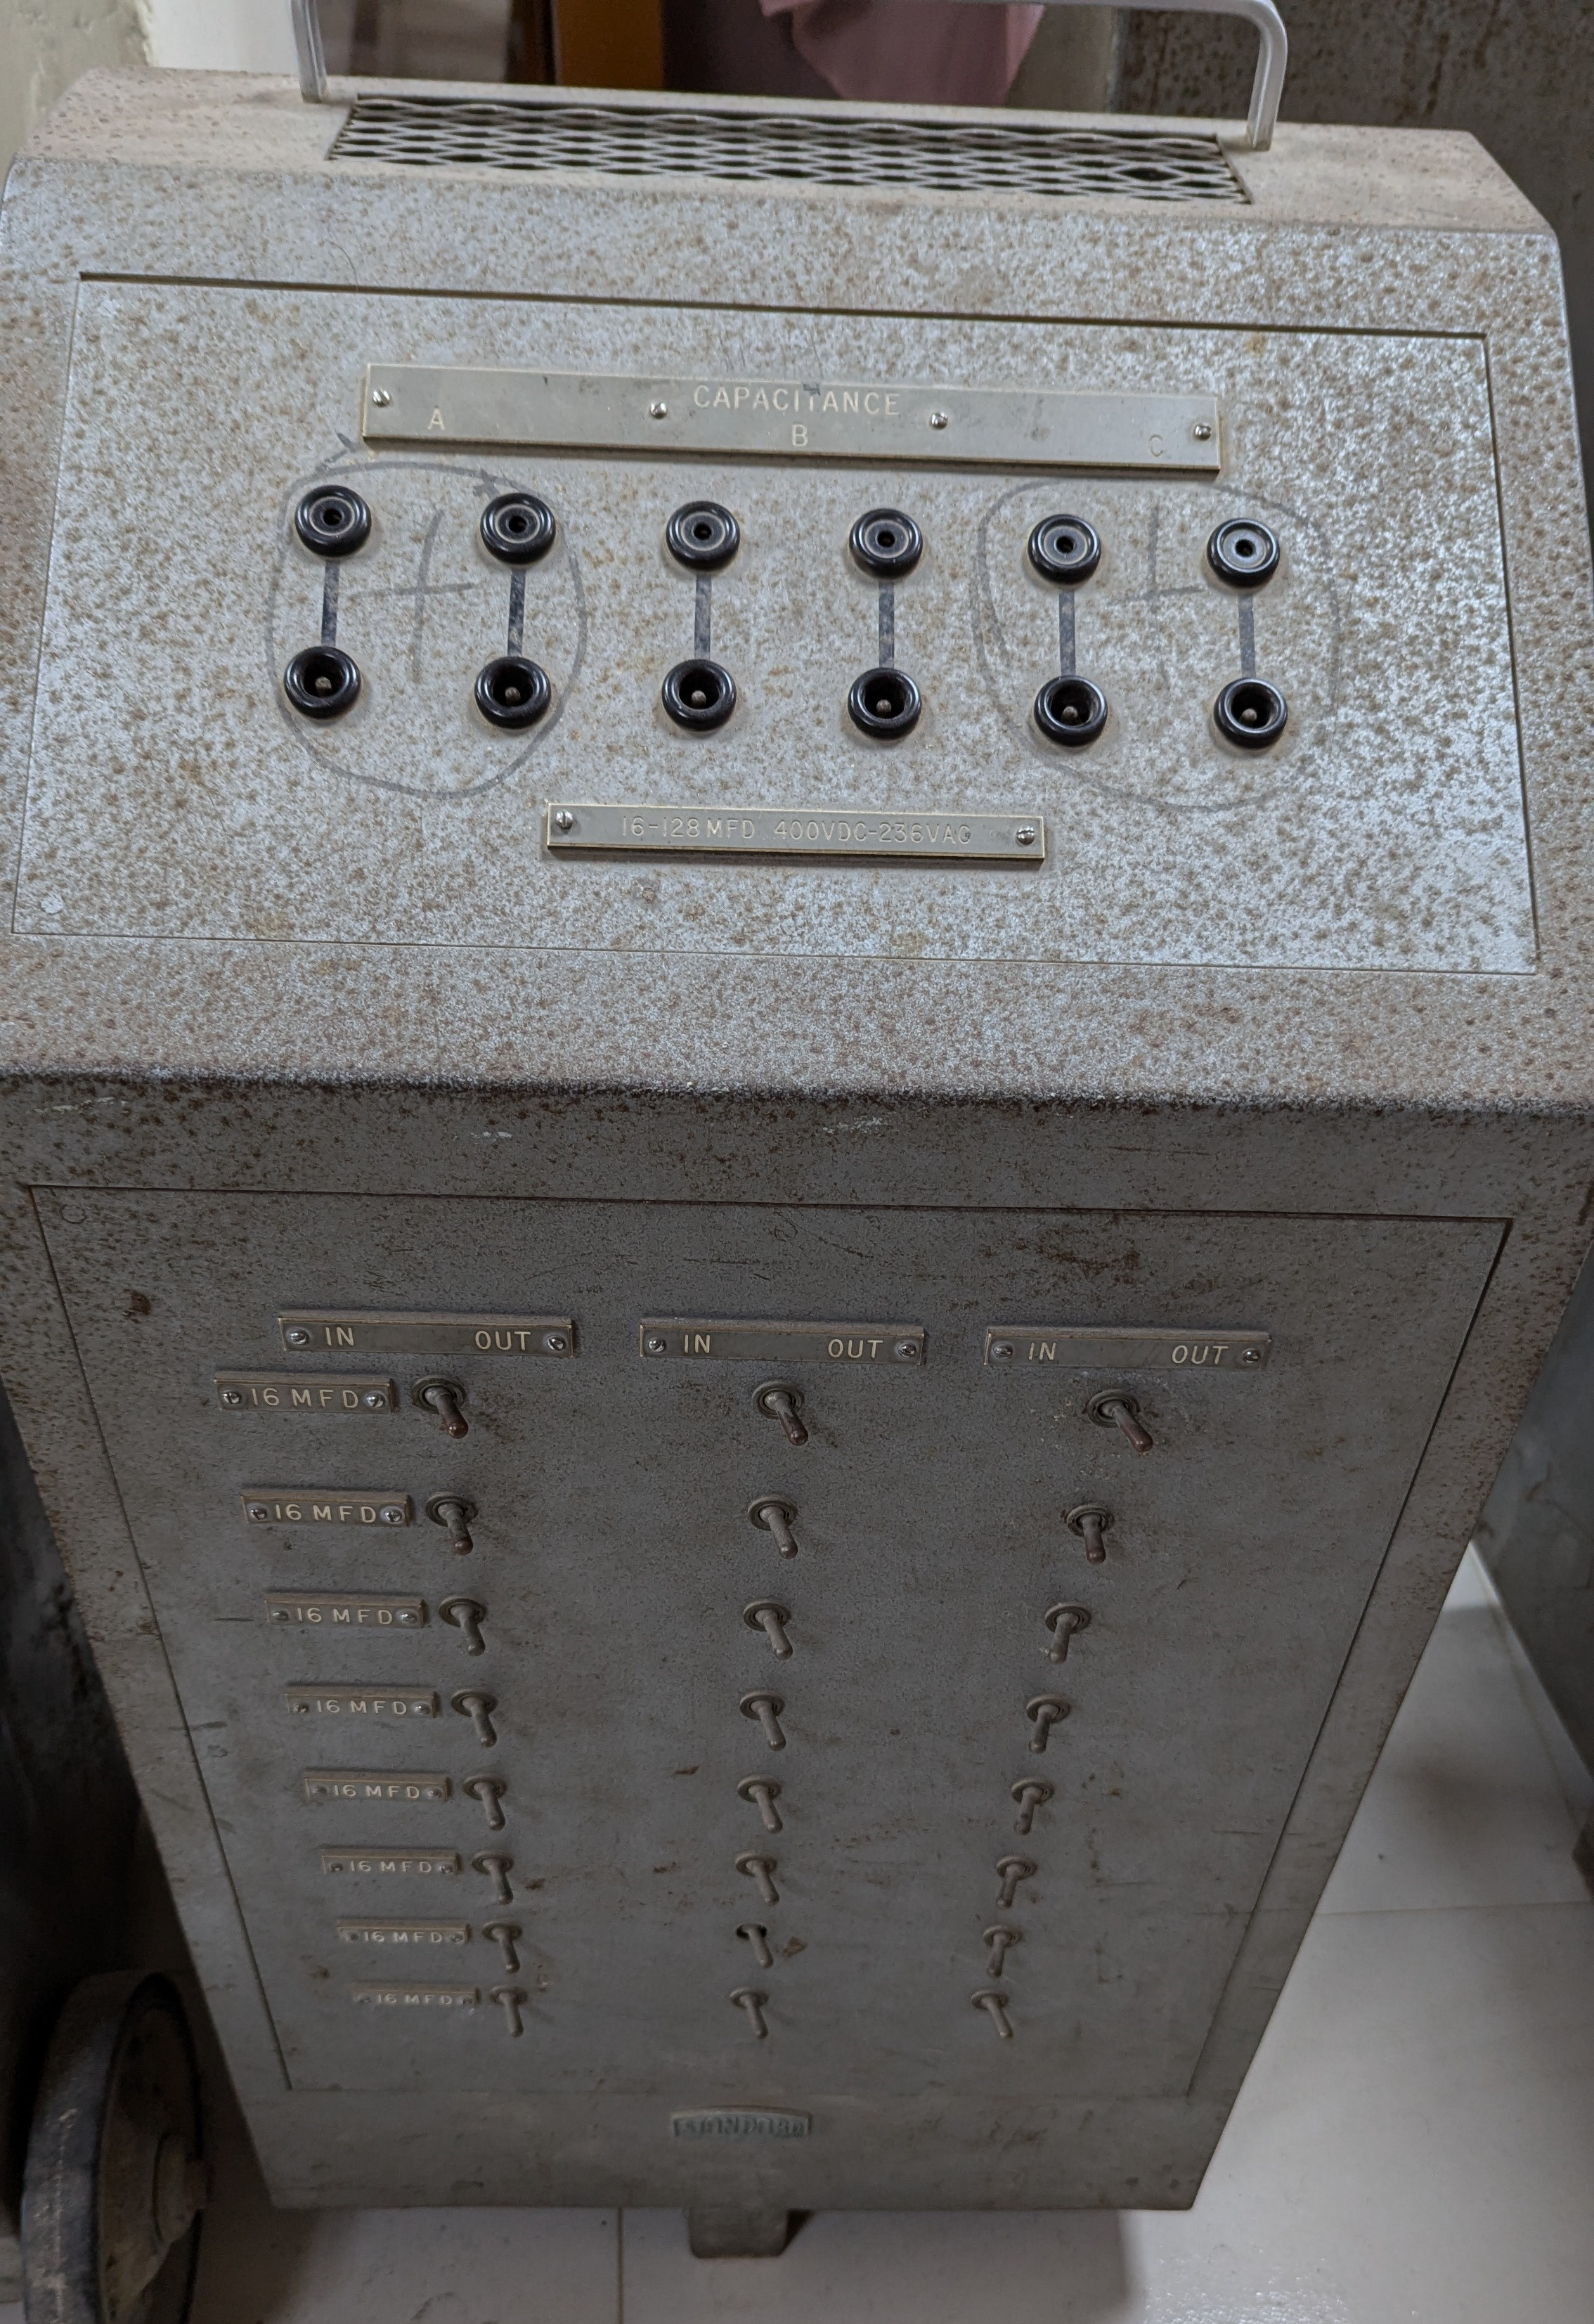
\includegraphics[width=1\linewidth]{Images/12}
			\caption{Front View}
		\end{subfigure}
		\hfill
		\begin{subfigure}[t]{0.32\textwidth}
			\centering
			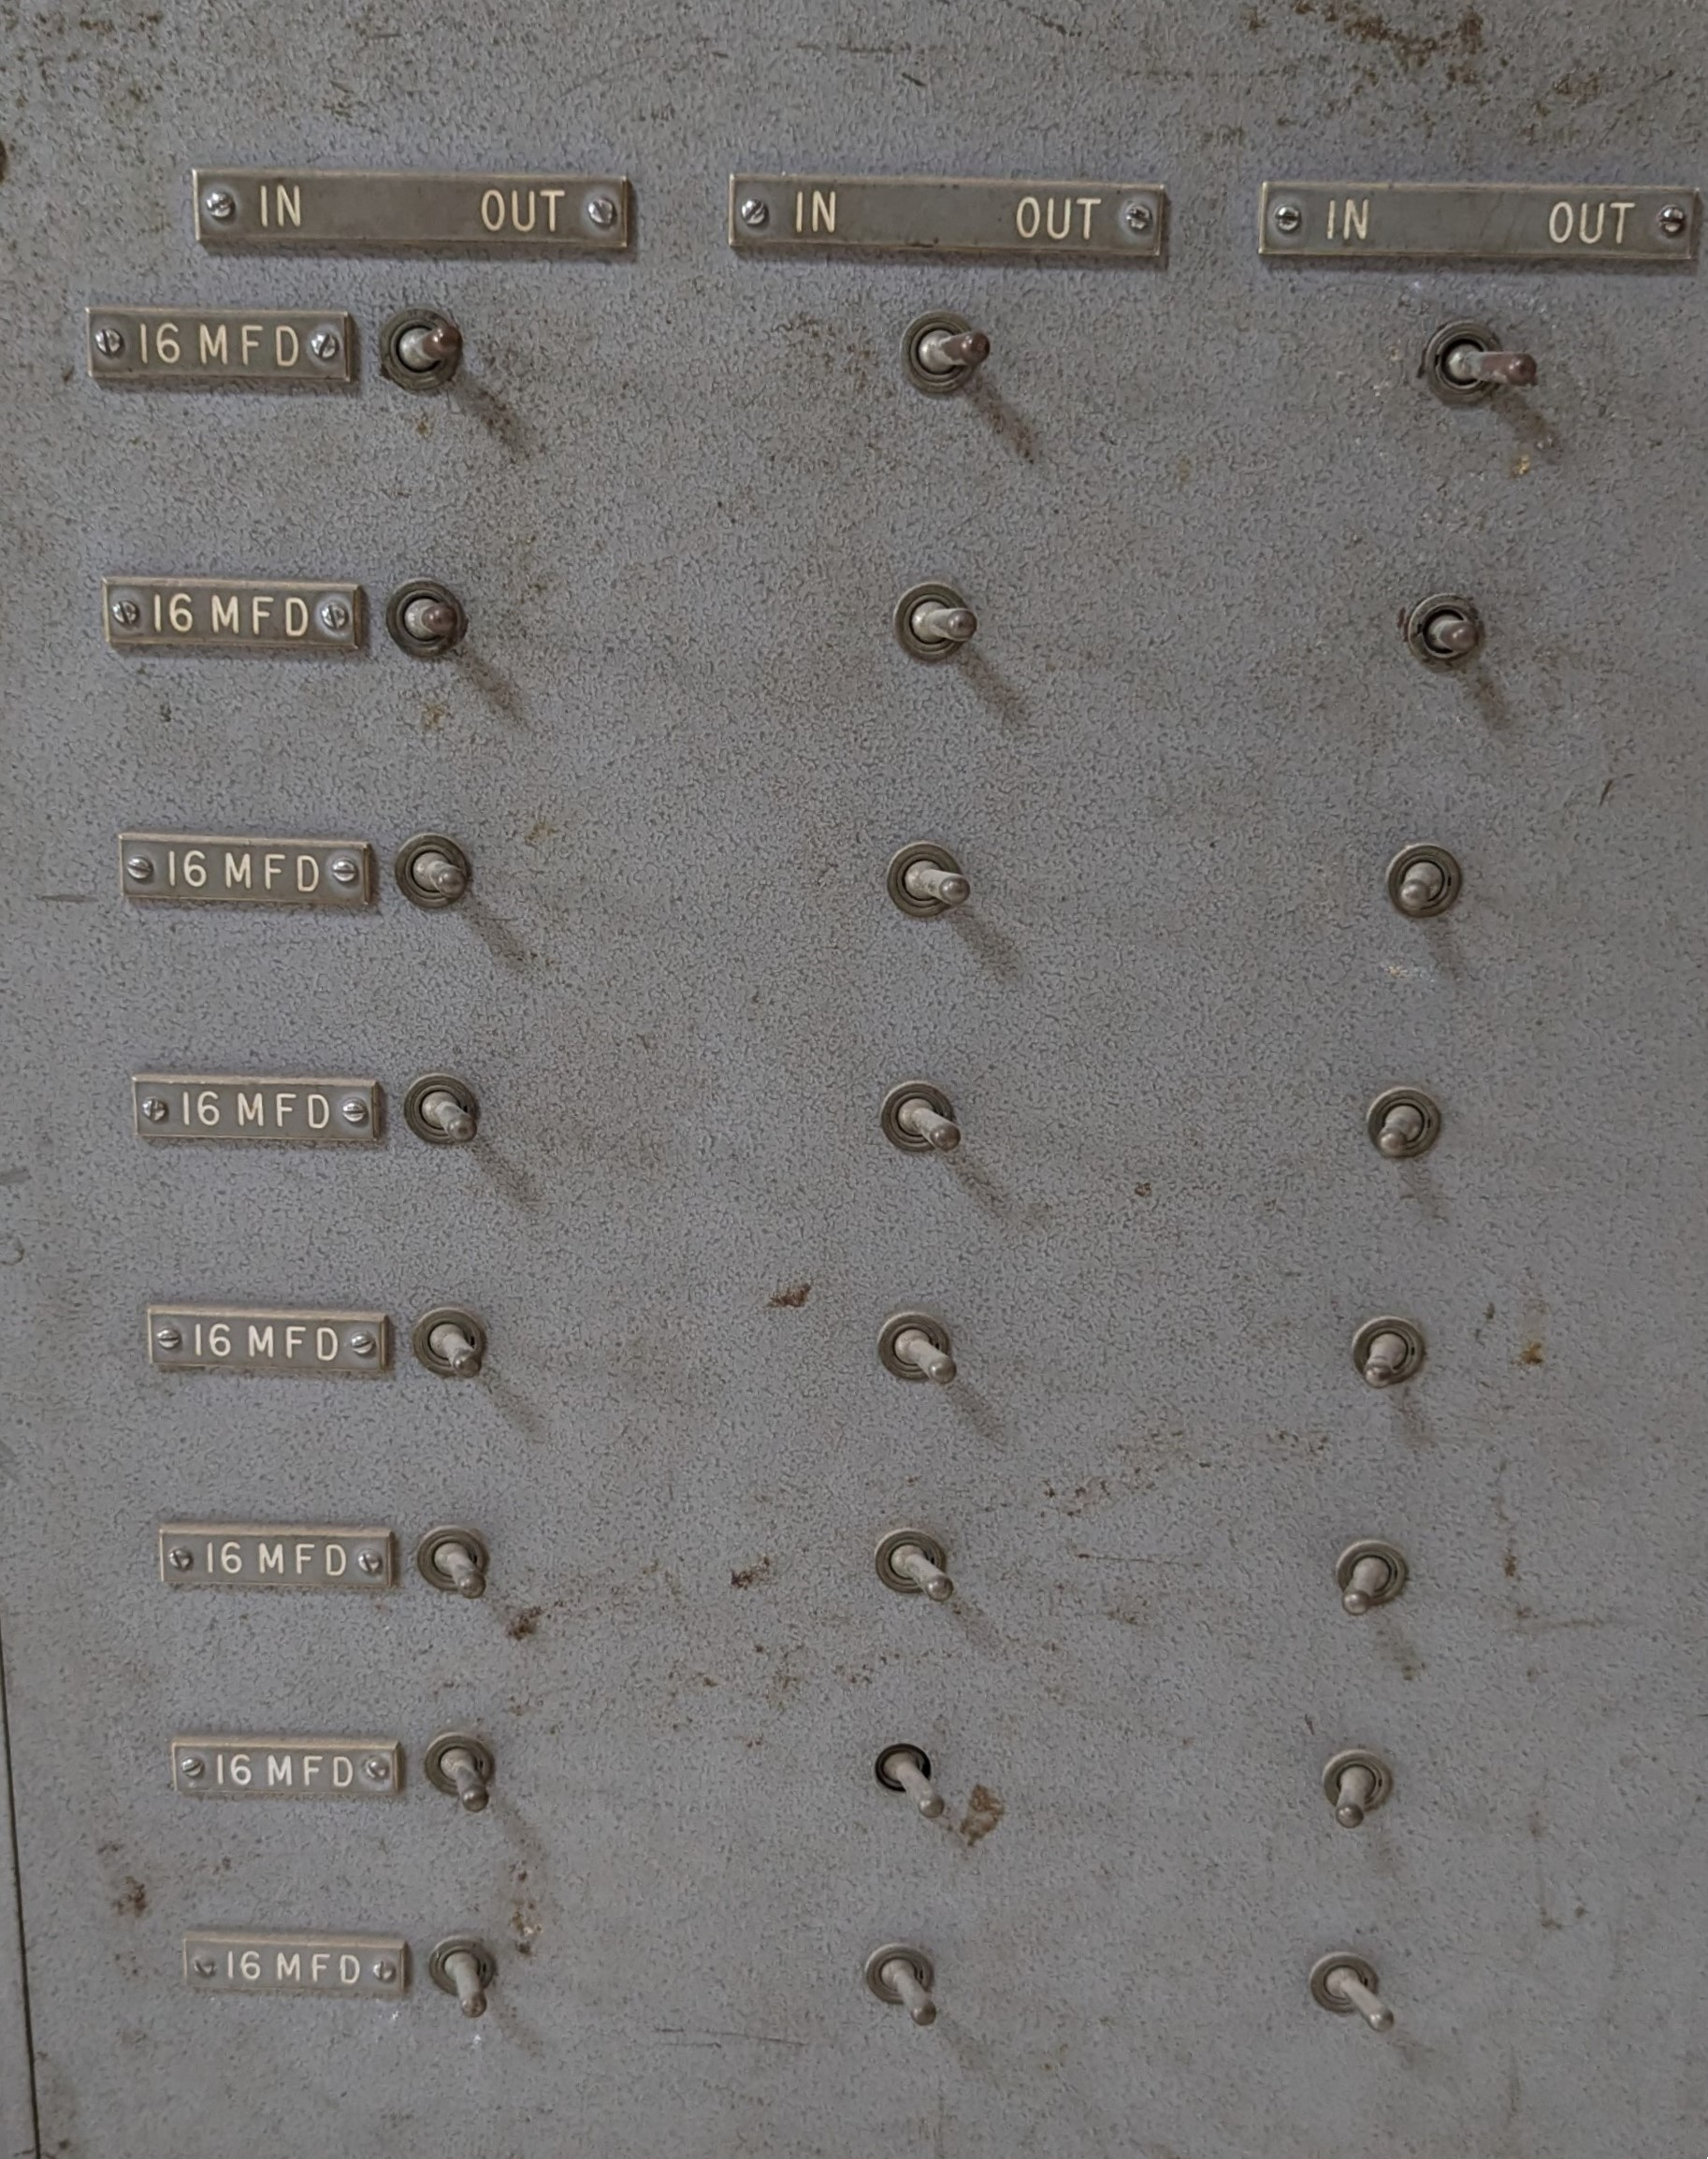
\includegraphics[width=1\linewidth]{Images/13}
			\caption{Switches for selecting capacitance}
		\end{subfigure}
		\hfill
		\begin{subfigure}[t]{0.32\textwidth}
			\centering
			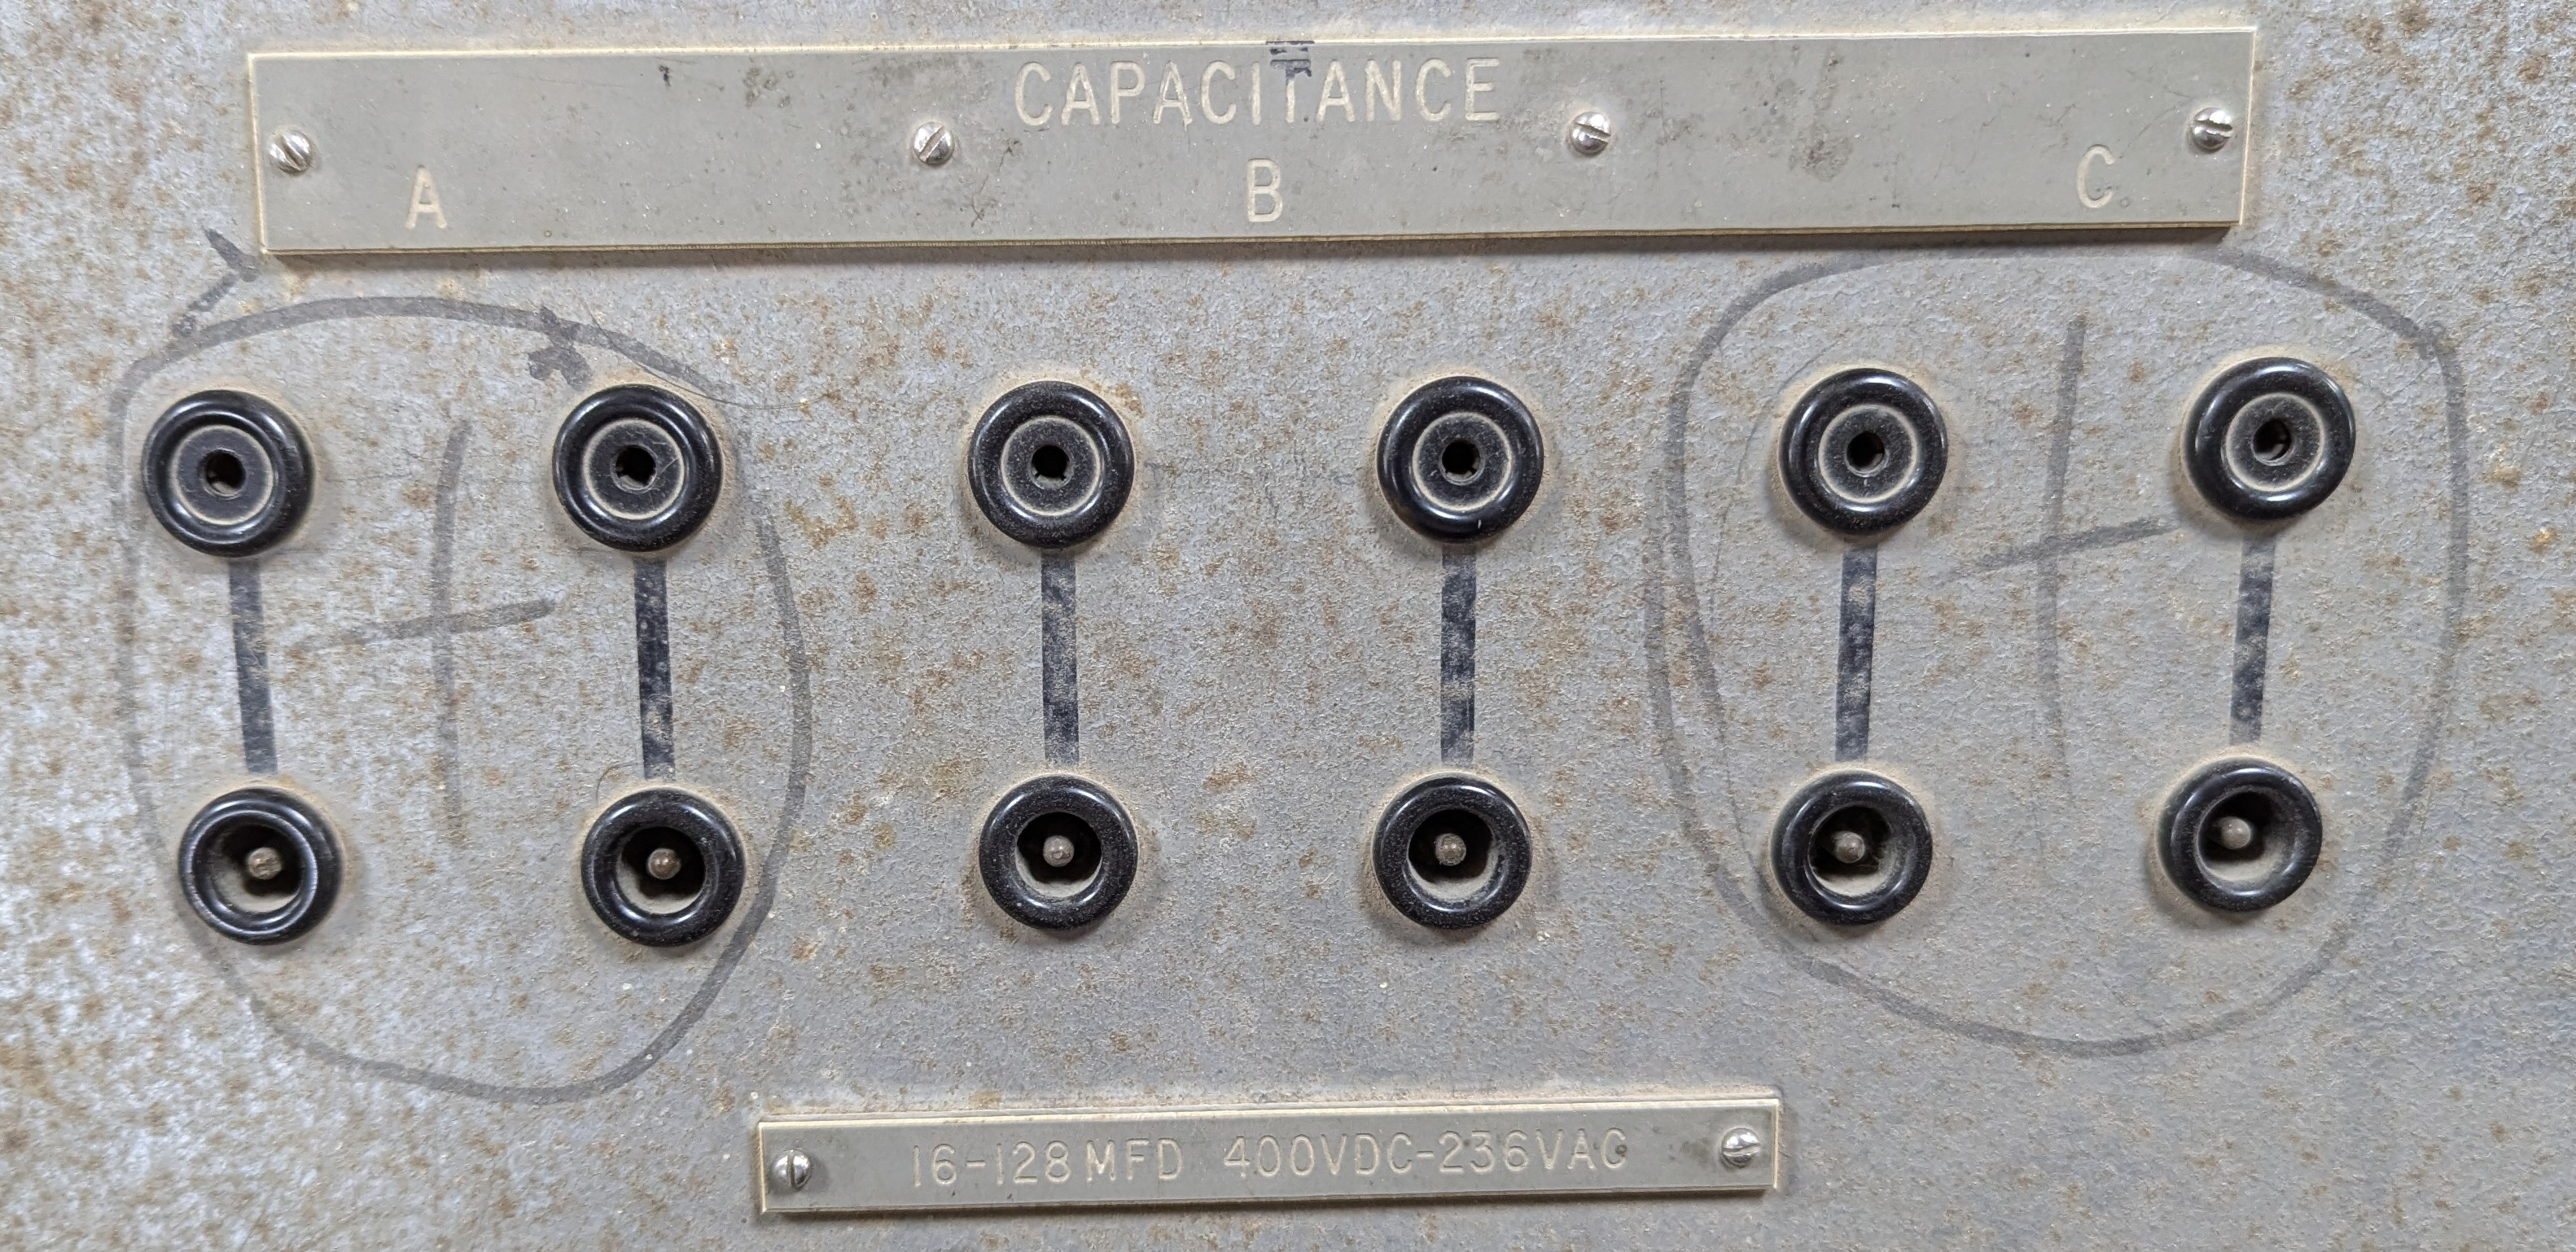
\includegraphics[width=1\linewidth]{Images/14}
			\caption{Top View}
		\end{subfigure}}
		
		\caption{Laboratory Capacitor with High Power Ratings}
		\label{fig:5}
	\end{figure}
	
	
\subsection{Multimeter}
A multimeter is a versatile electronic measuring instrument used to measure various electrical parameters, including voltage, current, and resistance. Multimeters can be either analog or digital, with digital multimeters (DMMs) offering more precise readings, faster response times, and additional features compared to their analog counterparts.

\subsubsection{Functions of a Multimeter}
A typical multimeter can measure:
\begin{itemize}
	\item \textbf{Voltage:} Measures both AC and DC voltage.
	\item \textbf{Current:} Measures both AC and DC current.
	\item \textbf{Resistance:} Measures resistance in ohms.
\end{itemize}
In addition to these primary functions, many modern multimeters include features such as:
\begin{itemize}
	\item \textbf{Continuity Testing:} Used to check if a circuit is complete, emitting a beep if continuity is present.
	\item \textbf{Diode Testing:} Measures the forward voltage drop of a diode.
	\item \textbf{Capacitance Measurement:} Measures the capacitance of a component.
	\item \textbf{Temperature Measurement:} Some multimeters include a thermocouple input for measuring temperature.
\end{itemize}

\subsubsection{Types of Multimeter}
\textbf{Analog Multimeter:} Uses a moving needle to display measurements on a scale. Although less common today, they are still valued for their ability to show trends and fluctuations in measurements. \\
\textbf{Digital Multimeter (DMM):} Provides accurate numerical readings on an LCD screen and is commonly used in modern applications due to its precision and additional functionality.



	
	
\begin{figure}[H]
	\centering
	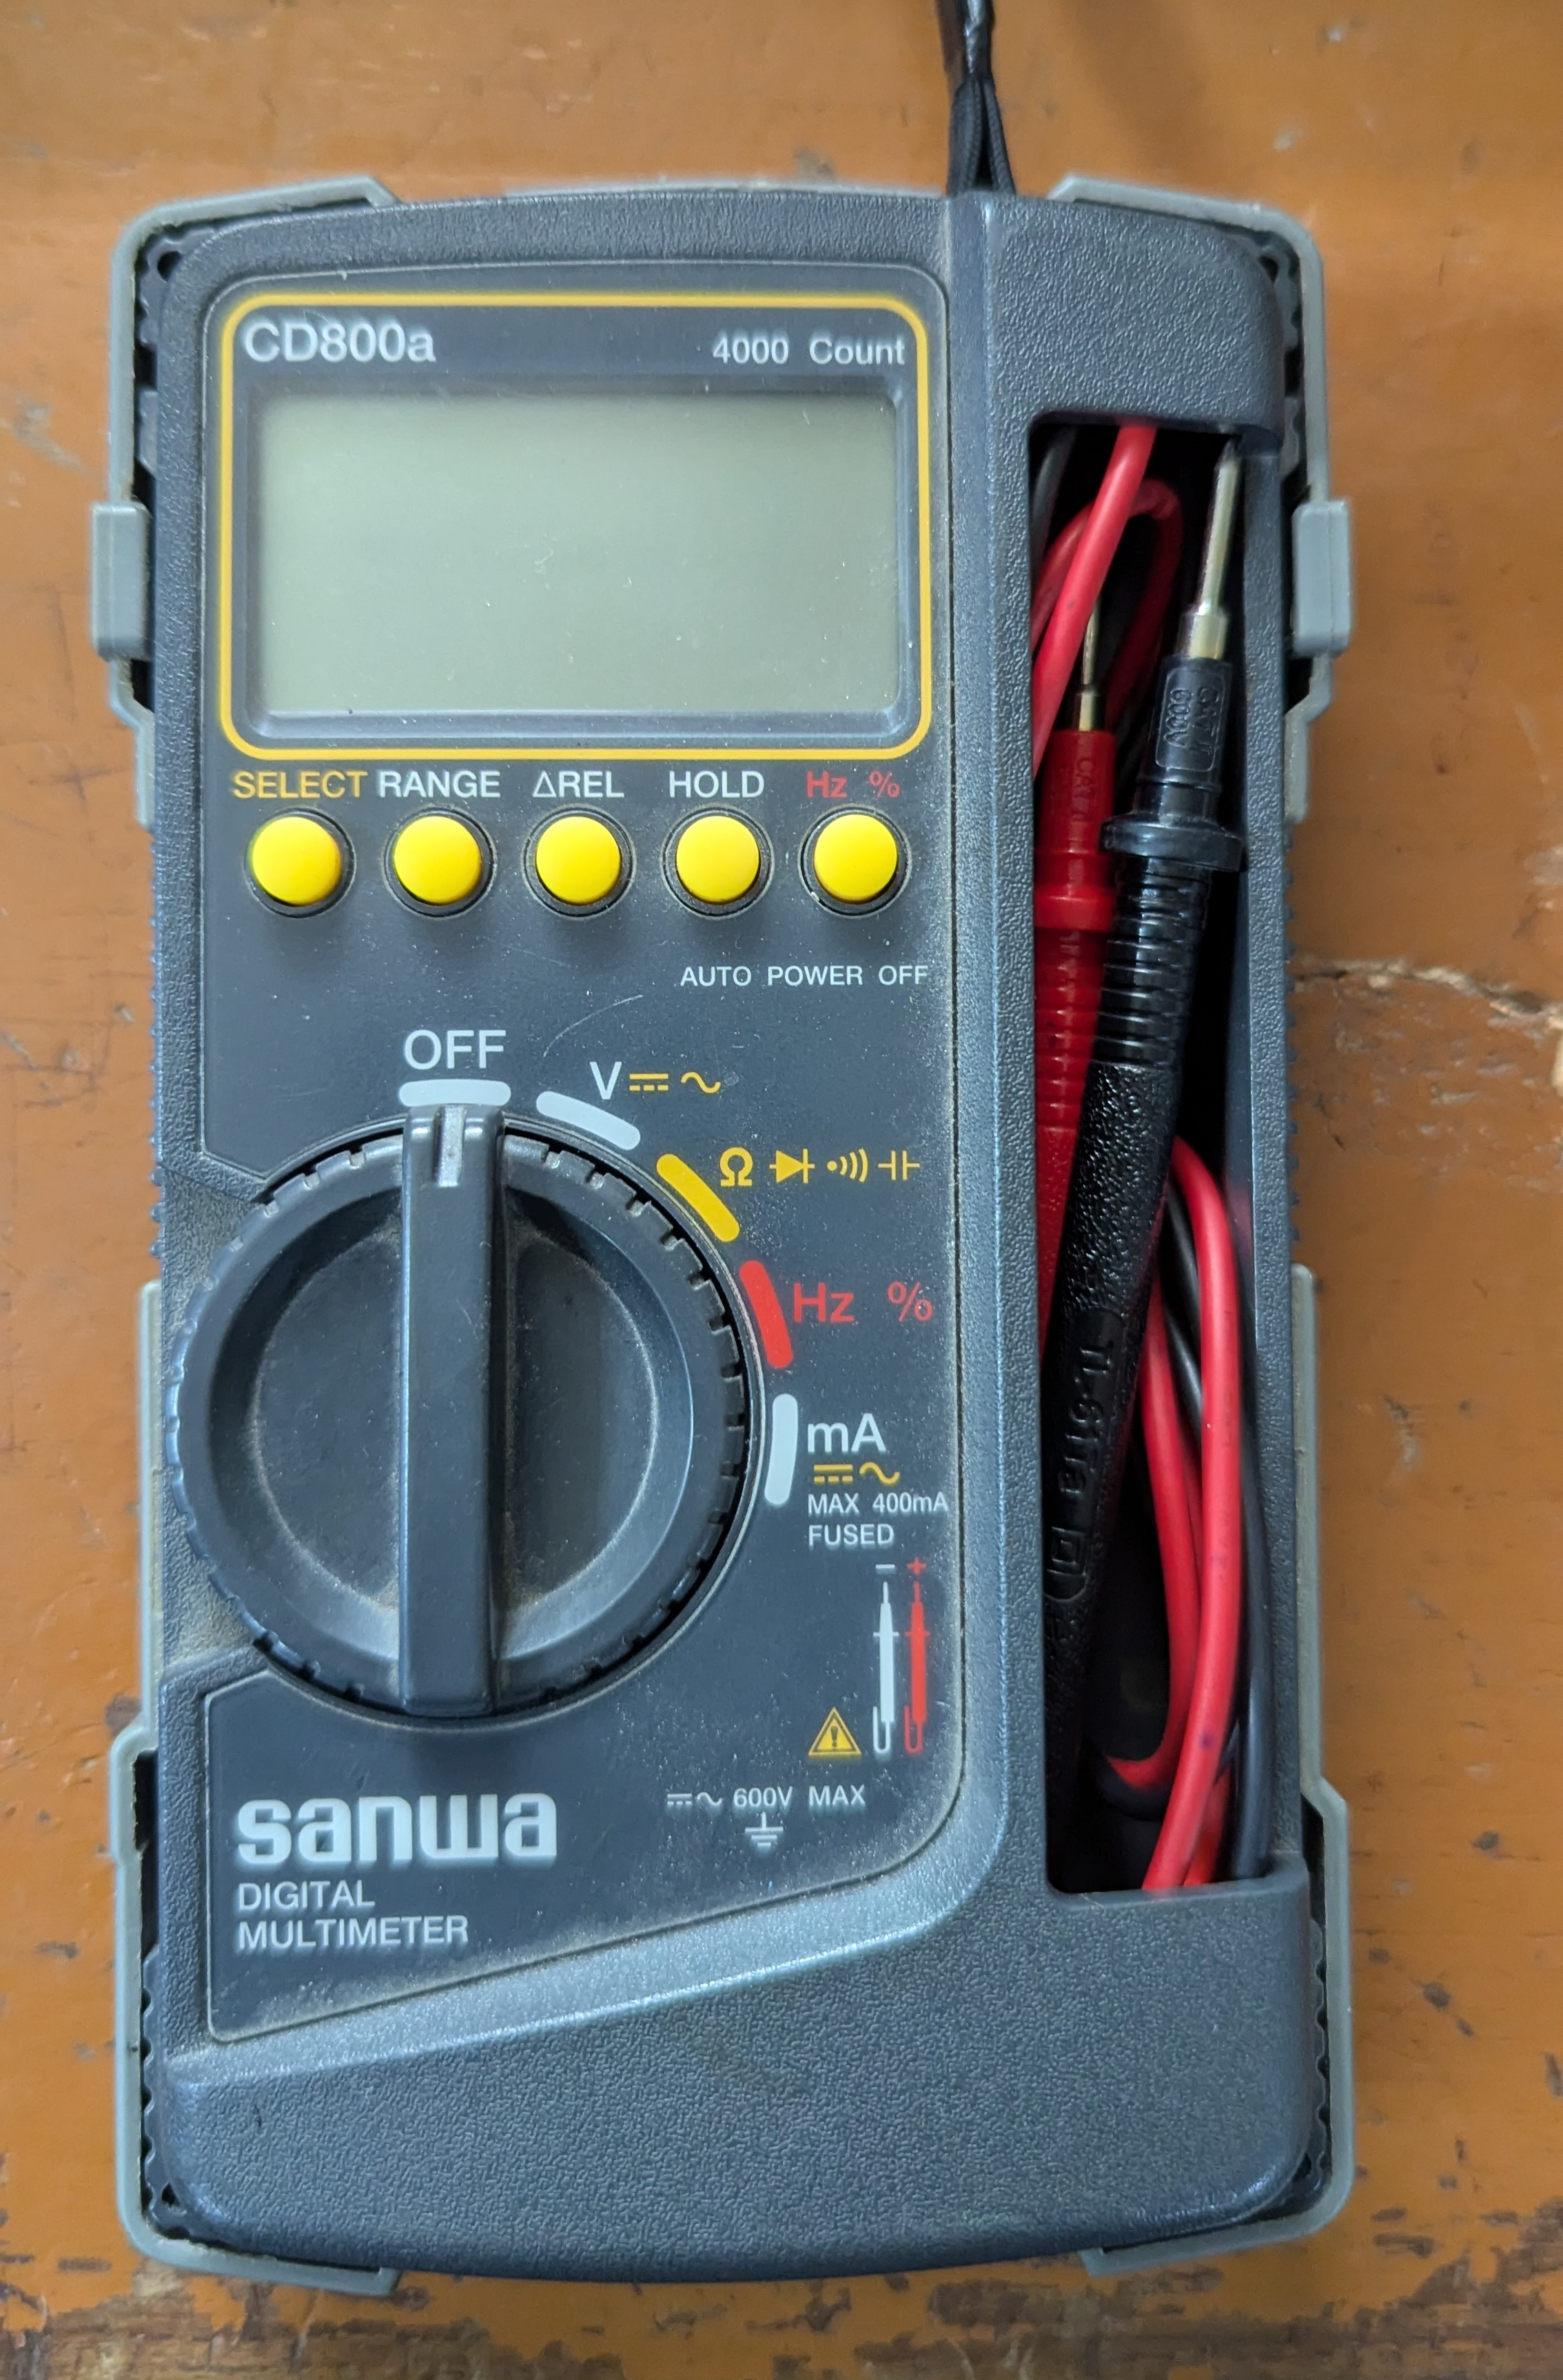
\includegraphics[angle=270,width=0.5\linewidth]{Images/4}
	\caption{Digital Multimeter}
	\label{fig:4}
\end{figure}
	
\subsection{Variac}
A variac, also known as a variable autotransformer, is a device used in laboratories to provide a variable AC voltage supply. It allows users to adjust the output voltage continuously from 0 to the maximum input voltage, typically 230V or 110V, depending on the model.\\
\textbf{Single-Phase Variac:} Designed for single-phase AC power supplies, it is commonly used in most lab applications to control voltage for testing and experiments.\\
\textbf{Three-Phase Variac:} Used in industrial settings, this type is designed for three-phase AC power systems and allows simultaneous control of voltage across all three phases.
		\begin{figure}[H]
		\centering
		\scalebox{1}{
		\begin{subfigure}[t]{0.49\textwidth}
			\centering
			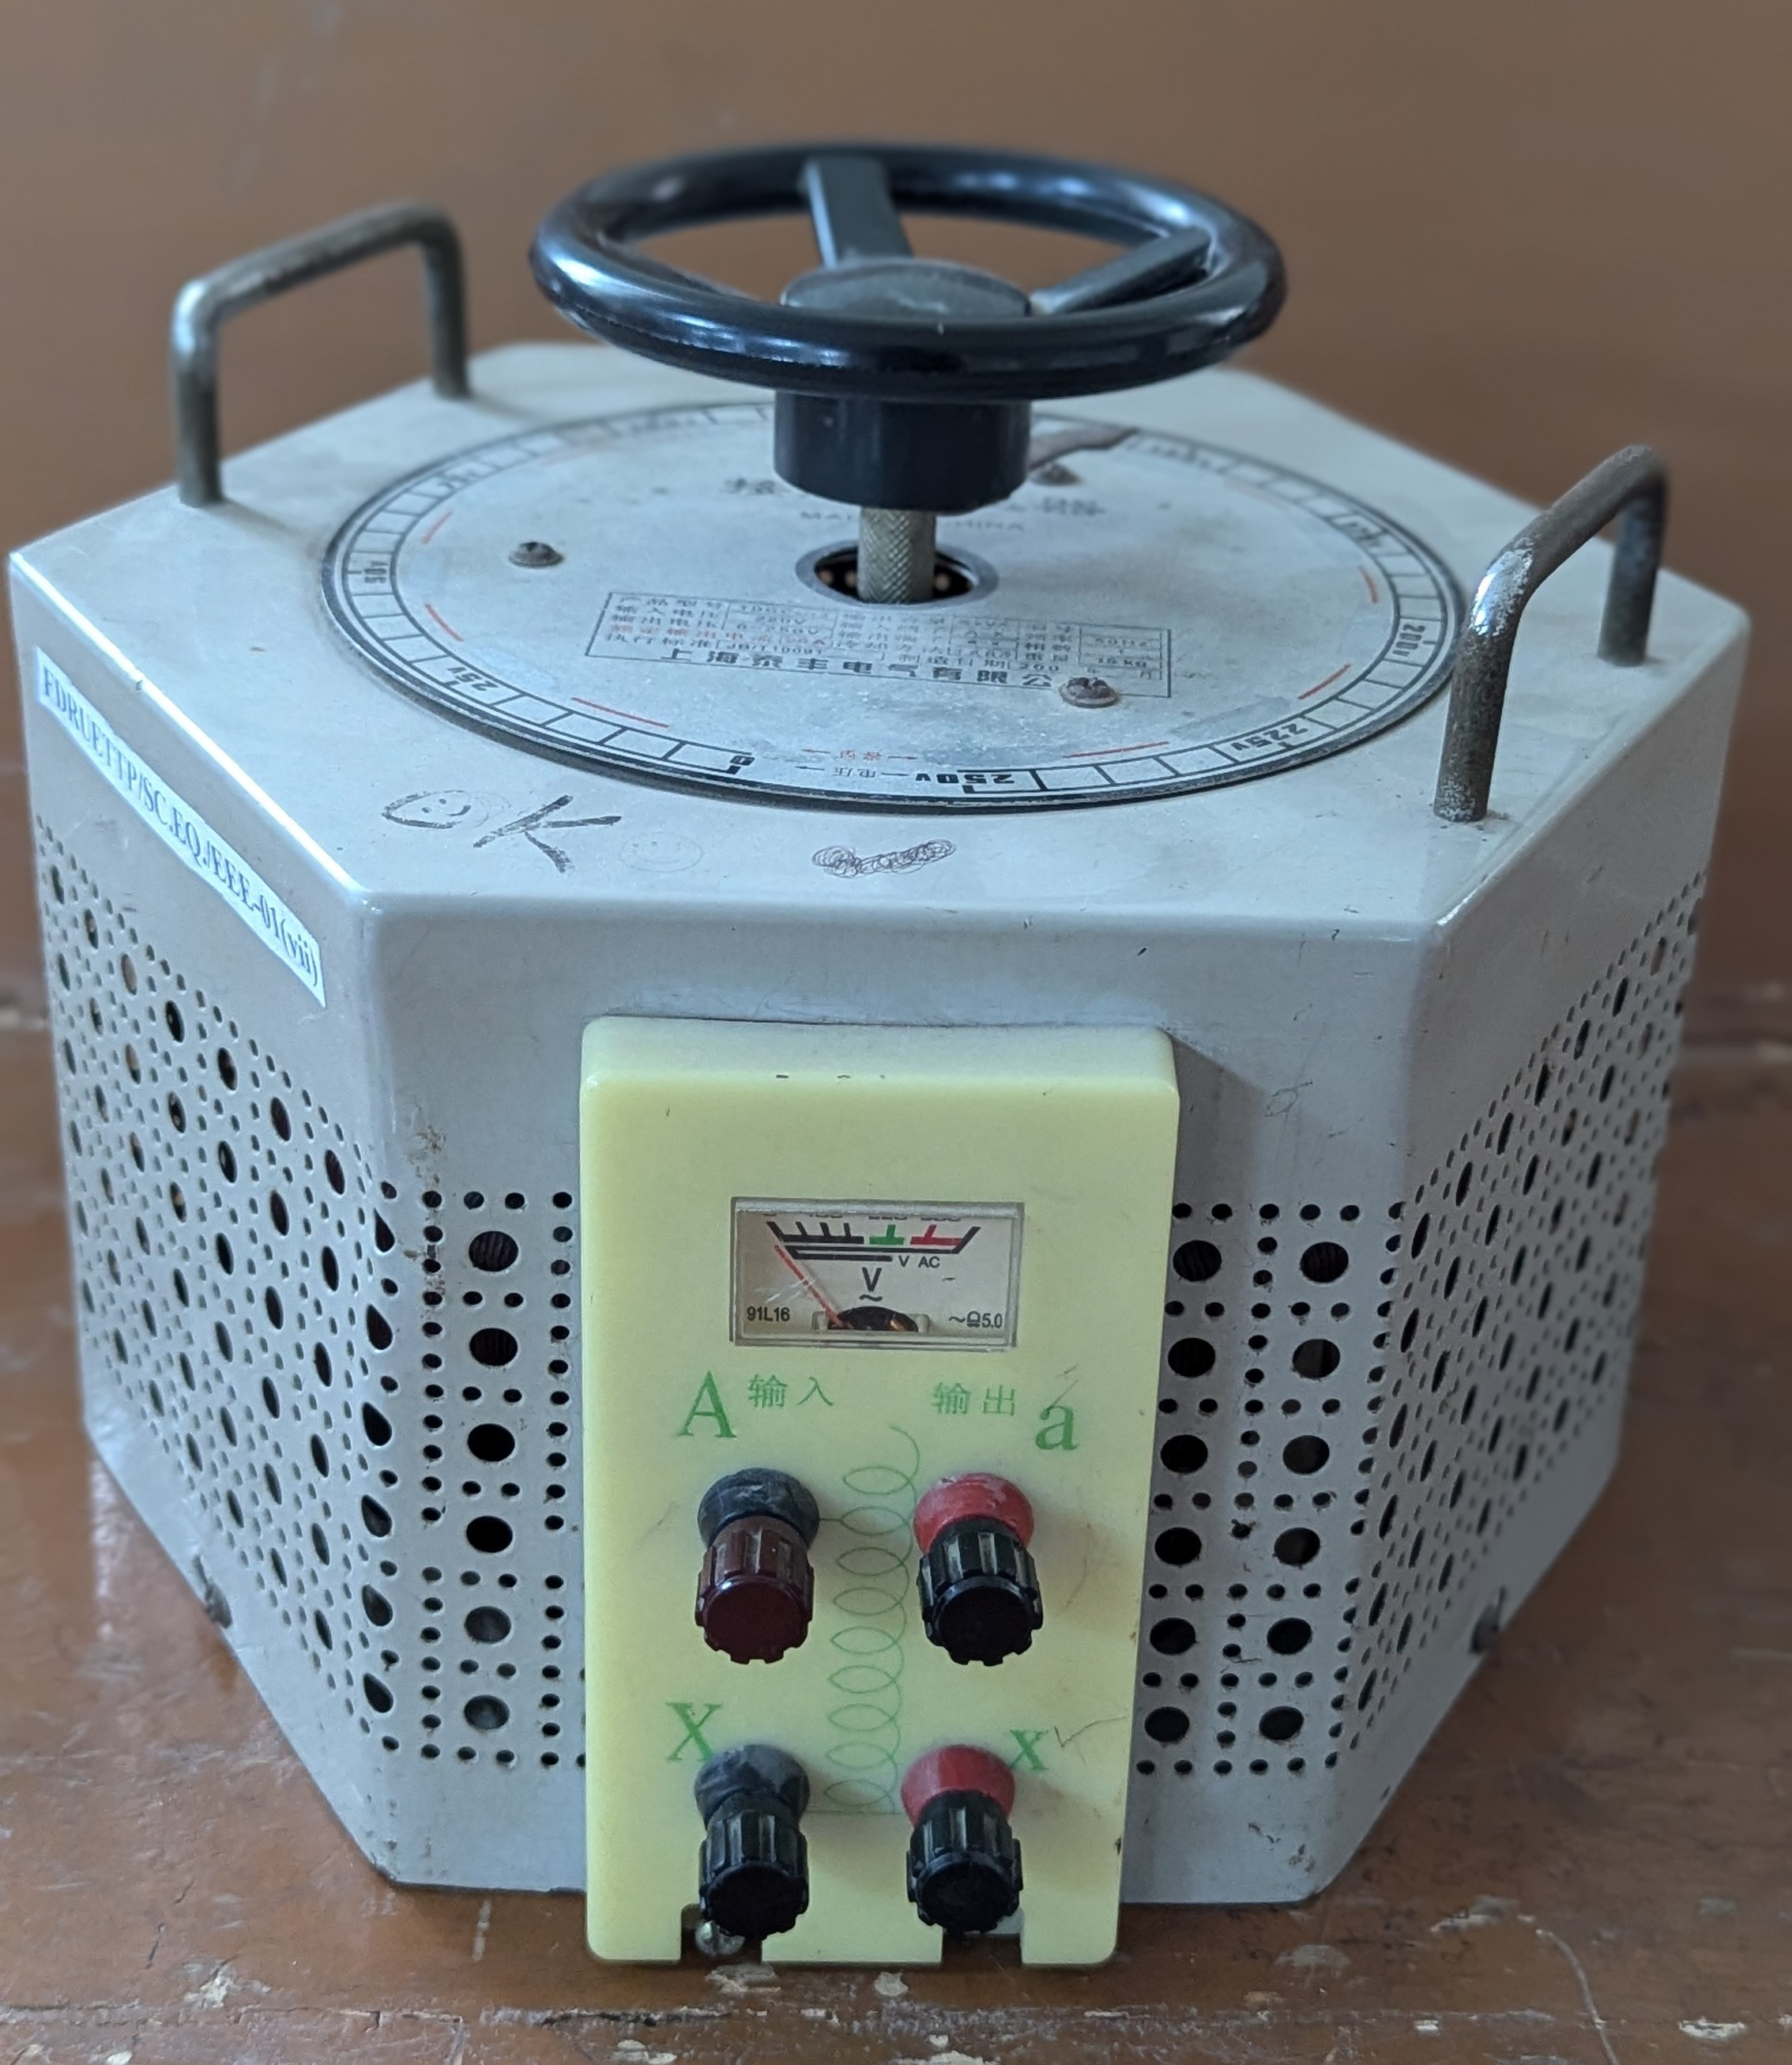
\includegraphics[width=.7\linewidth]{Images/15}
			\caption{Single-Phase Variac}
		\end{subfigure}
		\hfill
		\begin{subfigure}[t]{0.49\textwidth}
			\centering
			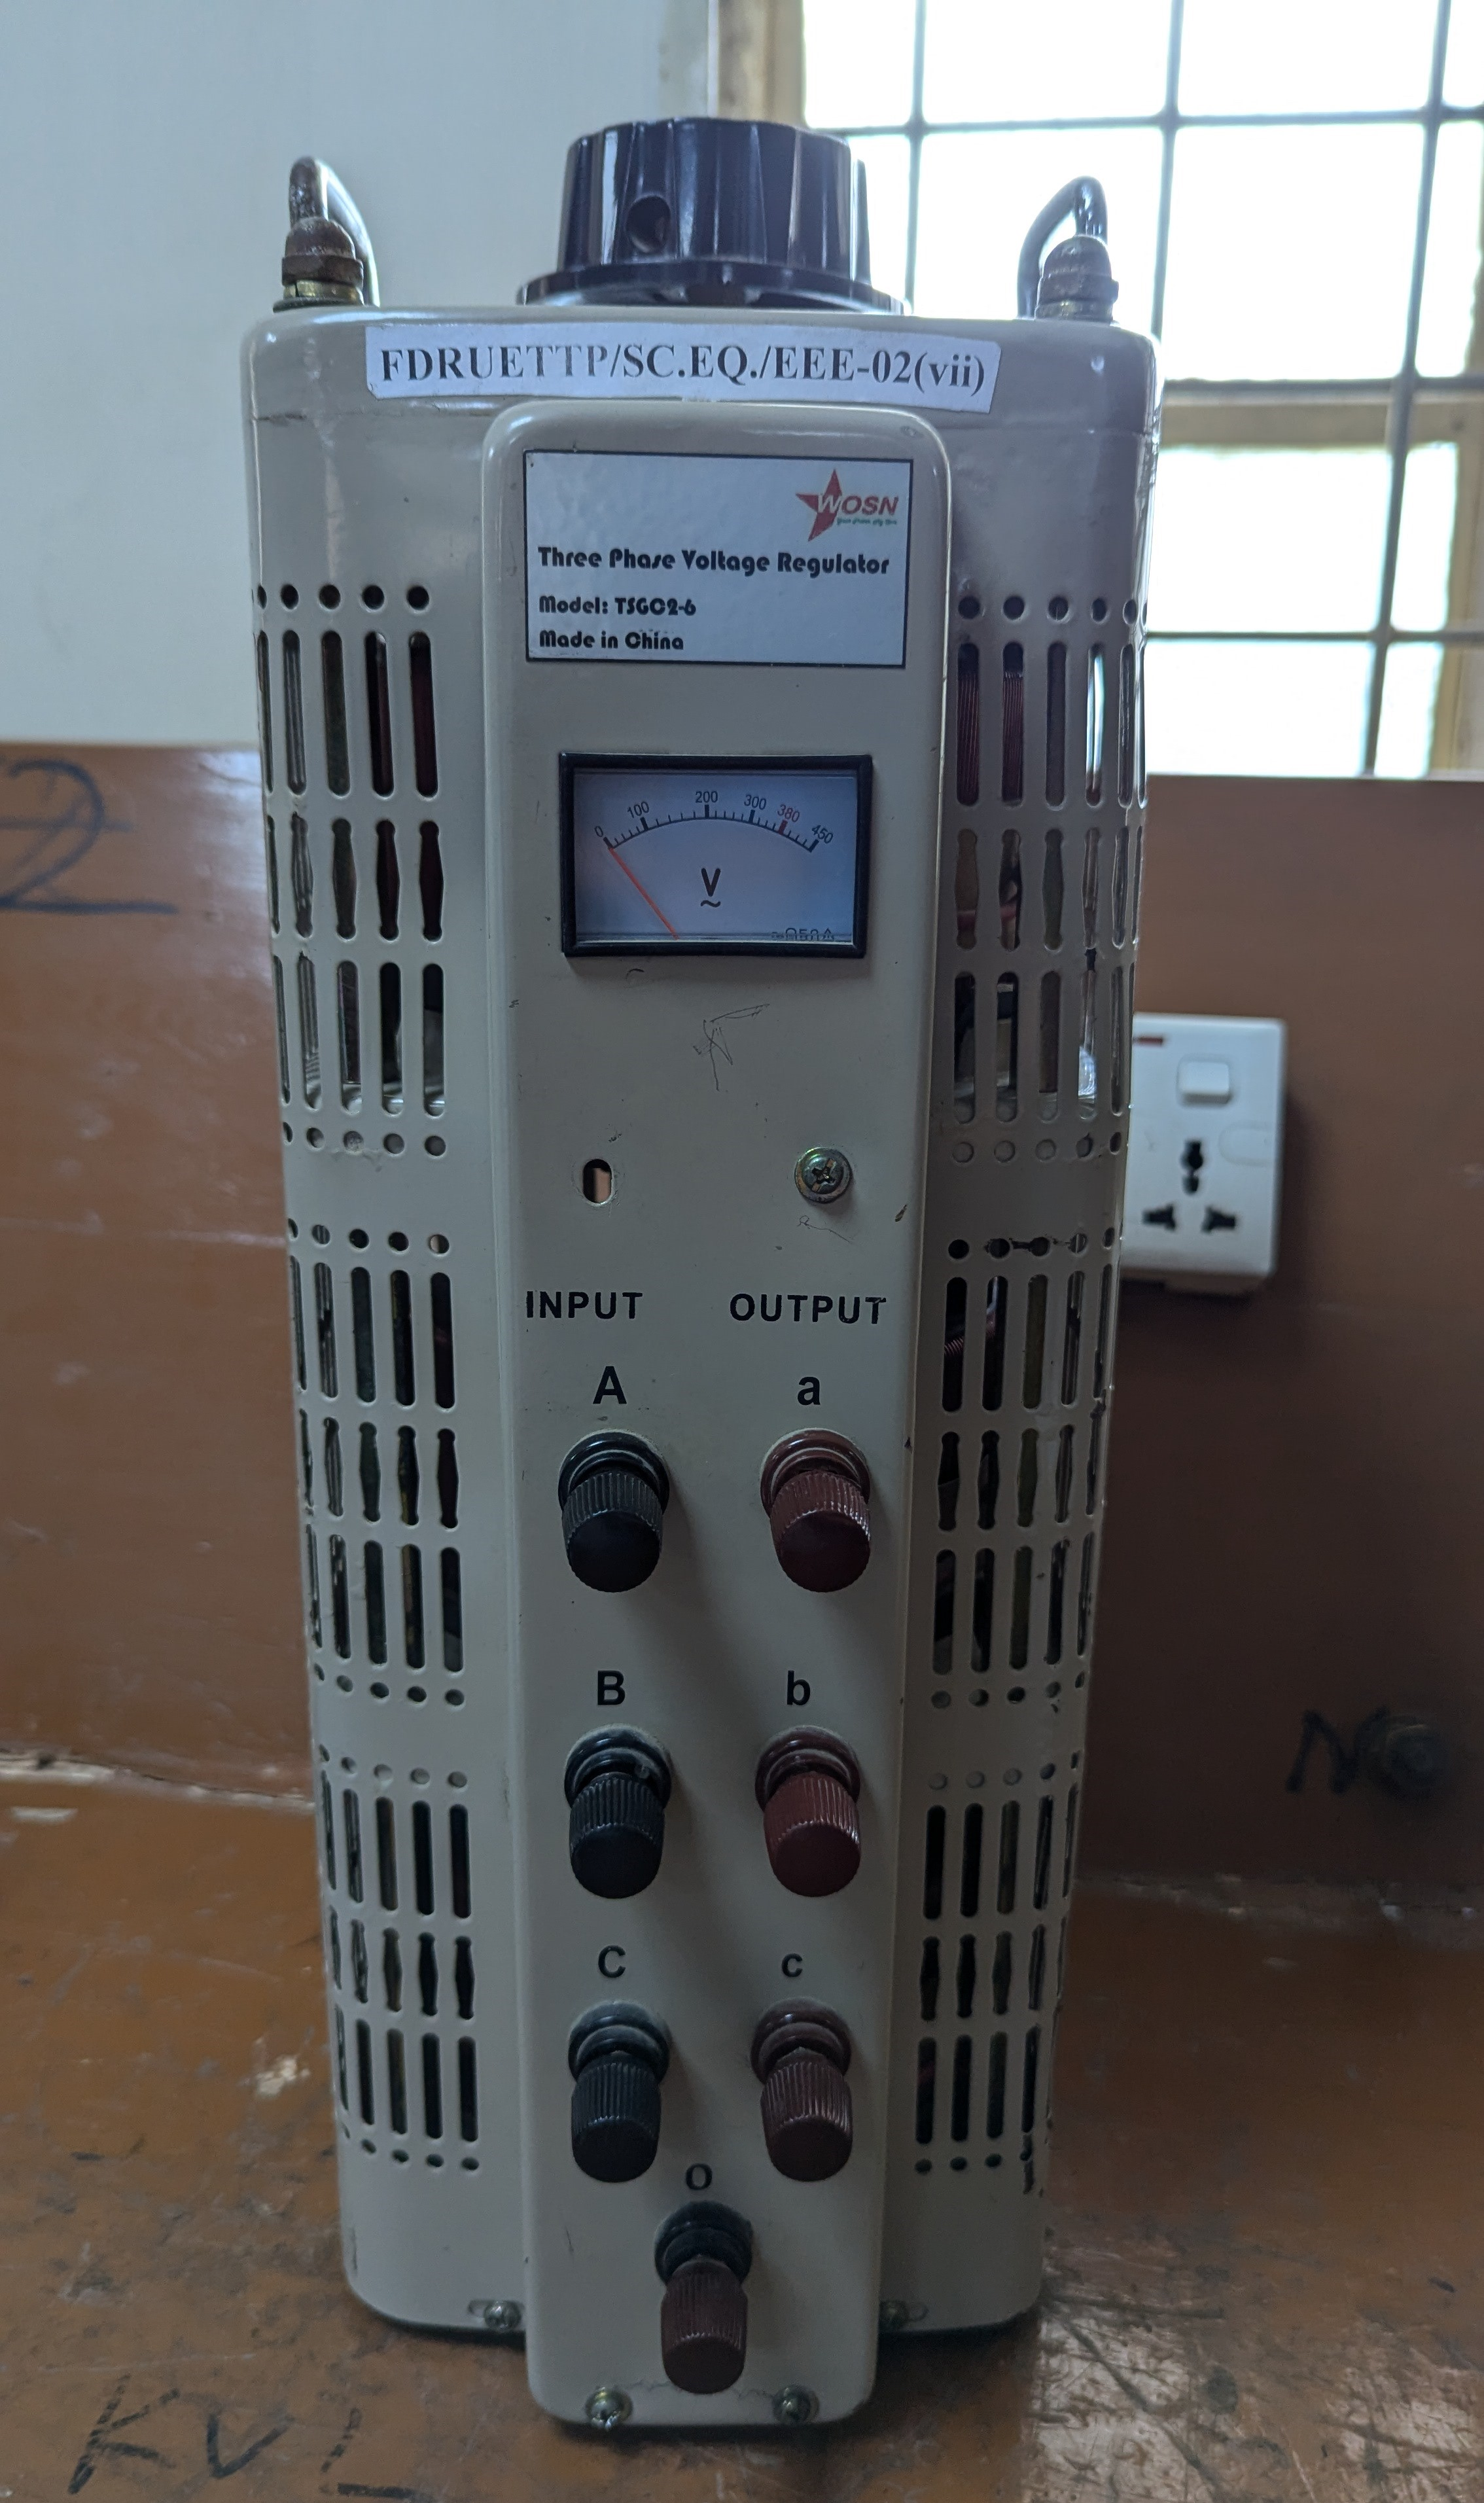
\includegraphics[width=.7\linewidth]{Images/16}
			\caption{Three-Phase Variac}
		\end{subfigure}}
		
		\caption{Variac}
		\label{fig:5}
	\end{figure}
\subsubsection{Working Principle}
A variac operates on the principle of electromagnetic induction. It consists of a single winding wound on a laminated iron core, with a sliding brush that moves across the winding. By rotating a dial, the brush taps different points on the winding, effectively changing the output voltage. Since it is an autotransformer, the primary and secondary windings are the same, but the voltage output varies based on the position of the brush. This allows for smooth and continuous adjustment of the output voltage without stepping through fixed increments.\\
Variacs are used in labs for equipment testing, voltage calibration, and in scenarios where adjustable AC voltage is required for experiments.
	\newpage
\subsection{Wattmeter}
A wattmeter is an instrument used to measure the electrical power consumed by a circuit, expressed in watts (W). It calculates power by measuring both the voltage across and the current through the circuit, while also accounting for the phase difference between them in alternating current (AC) circuits.\\
A wattmeter typically consists of two sets of coils:
\begin{itemize}
	\item \textbf{Voltage Coil:} Connected in parallel with the load to measure the voltage across the load.
	\item \textbf{Current Coil:} Connected in series with the load to measure the current flowing through the load.
\end{itemize}

\subsubsection{Working Principle}
In direct current (DC) circuits, power is calculated as the simple product of voltage and current:
\[
P = V \times I
\]
where \( P \) is power, \( V \) is voltage, and \( I \) is current.

In alternating current (AC) circuits, the wattmeter measures the real power by considering the power factor, which accounts for the phase difference between the voltage and current. The real power is given by:
\[
P = V \times I \times \cos(\phi)
\]
where \( \phi \) is the phase angle between the voltage and current.

\subsubsection{Laboratory Specifications}
In our laboratory, the wattmeter is rated for:
\begin{itemize}
	\item \textbf{Current:} 2/10 A
	\item \textbf{Voltage:} 120/240 V
\end{itemize}


	\begin{figure}[H]
		\centering
		\begin{subfigure}[t]{0.33\textwidth}
			\centering
			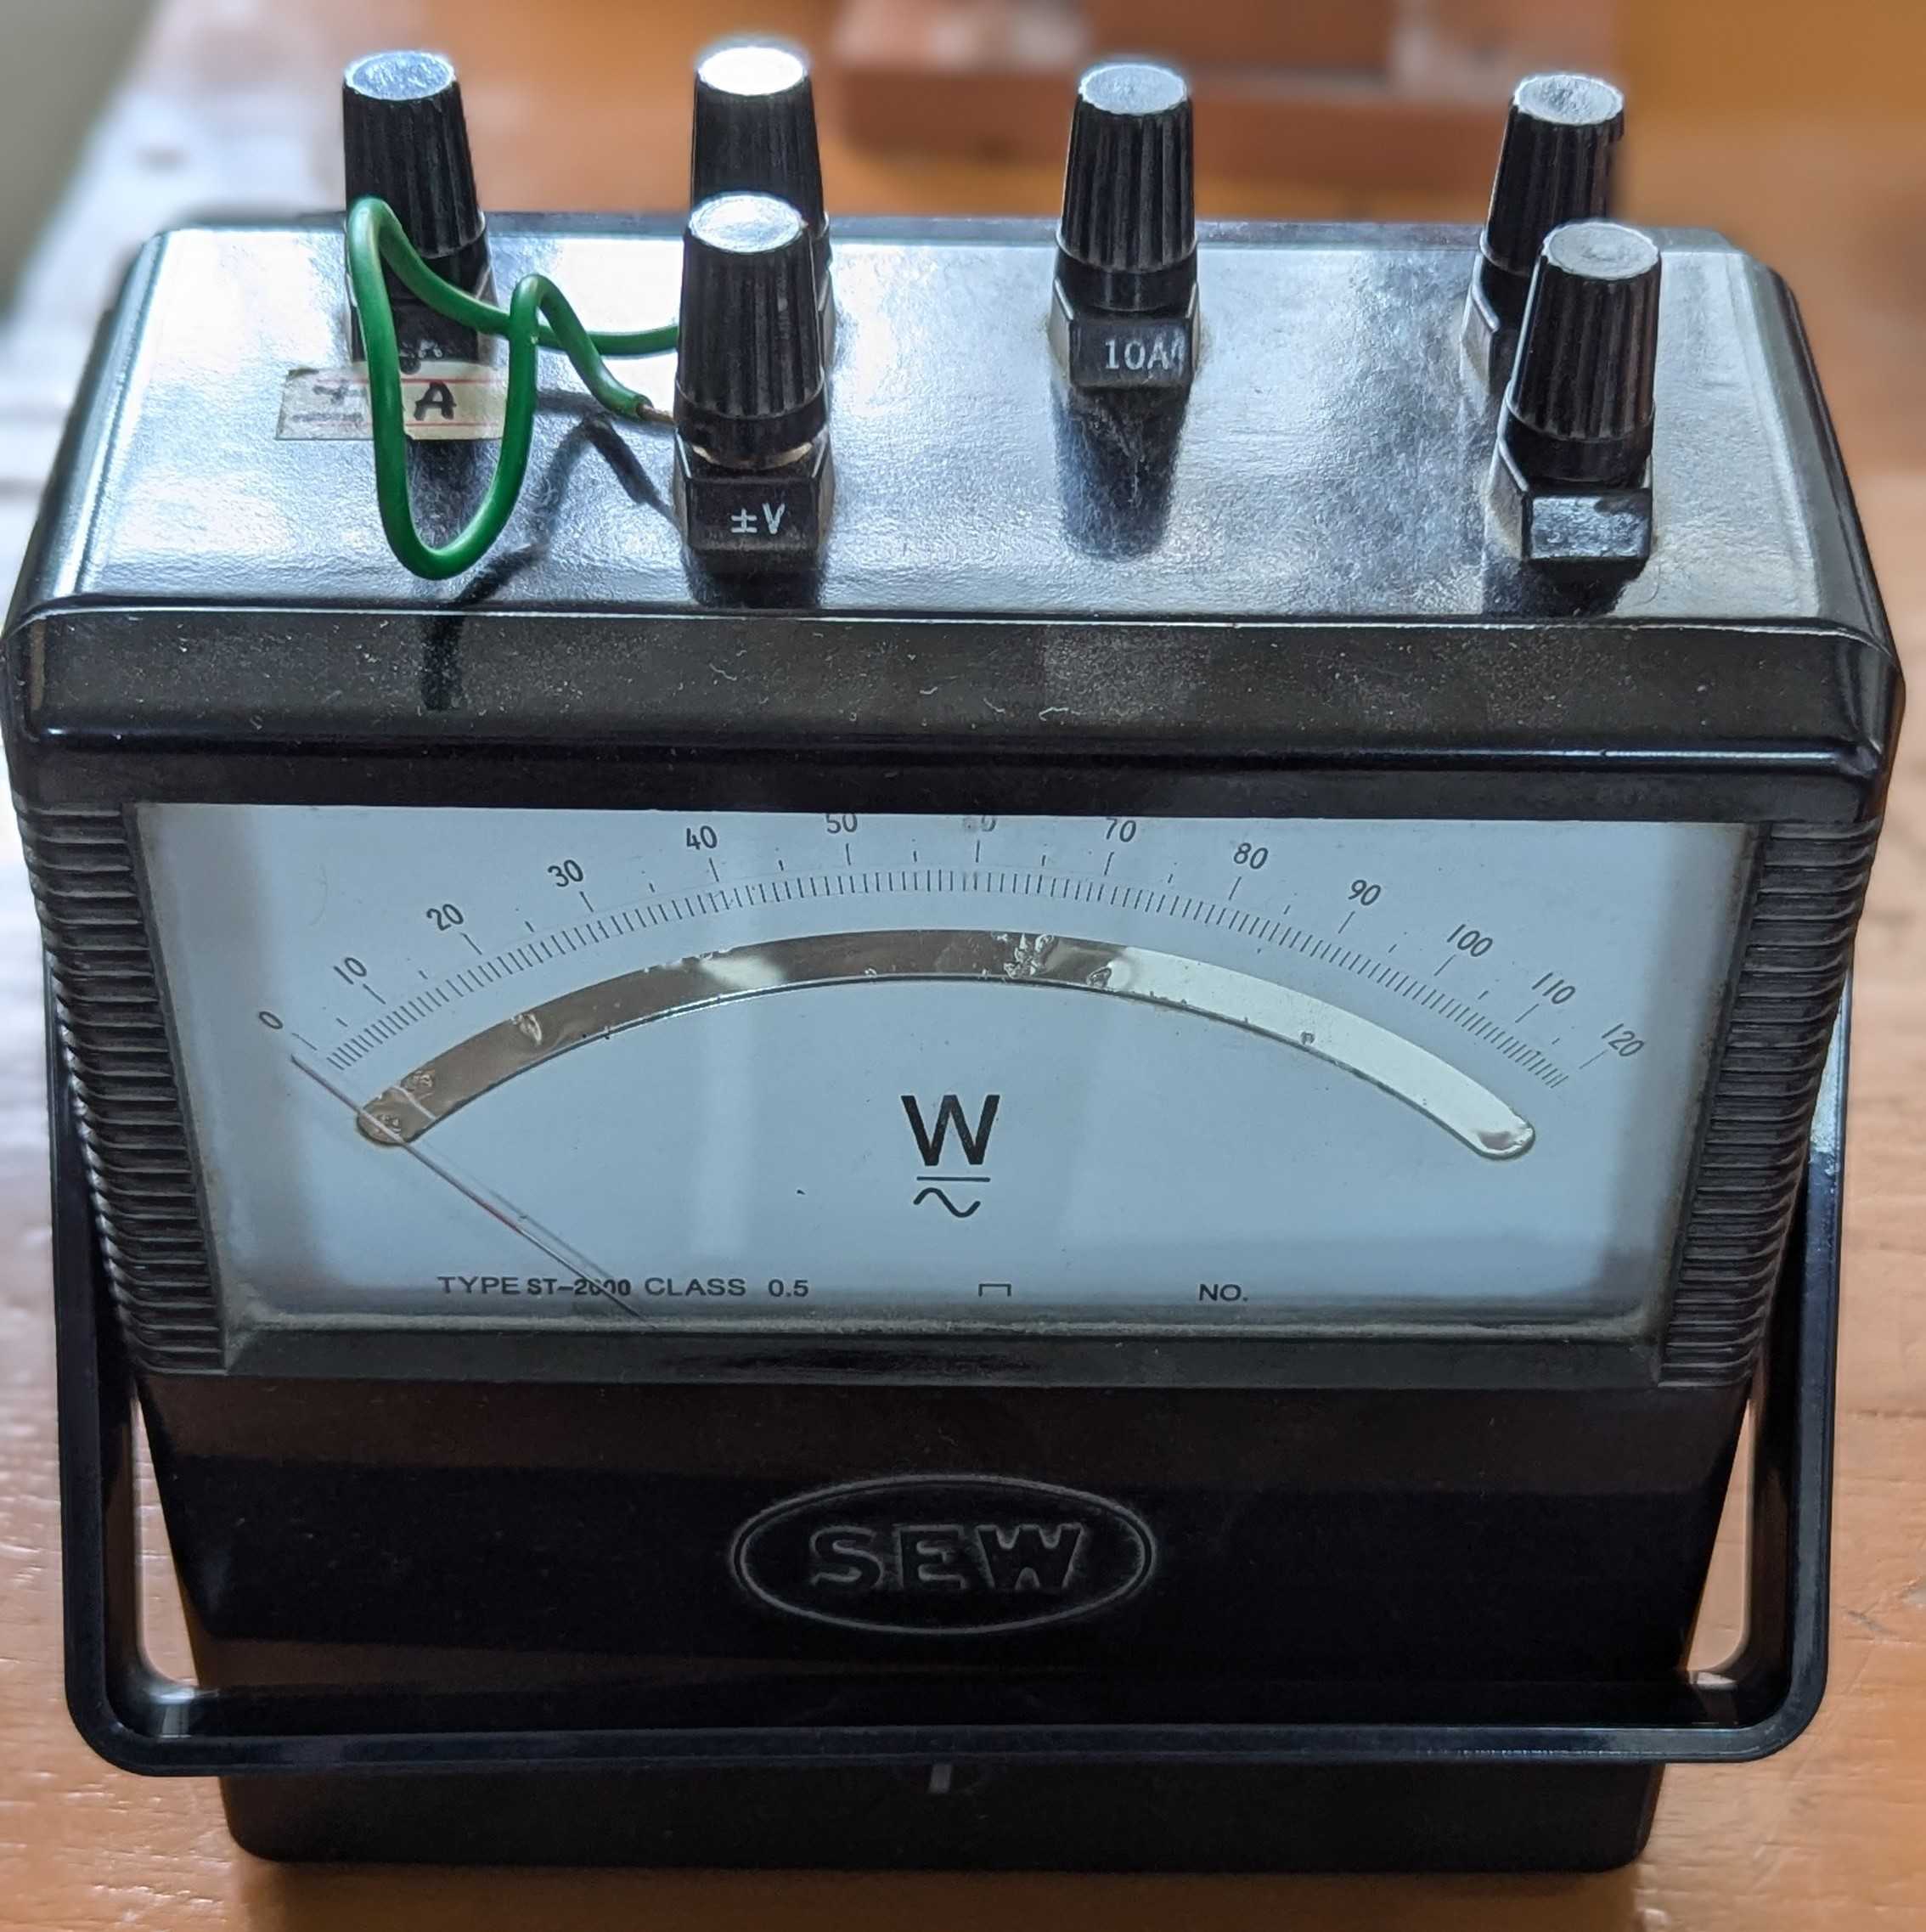
\includegraphics[width=1\linewidth]{Images/18}
			\caption{Front View}
		\end{subfigure}
		\hfill
		\begin{subfigure}[t]{0.33\textwidth}
			\centering
			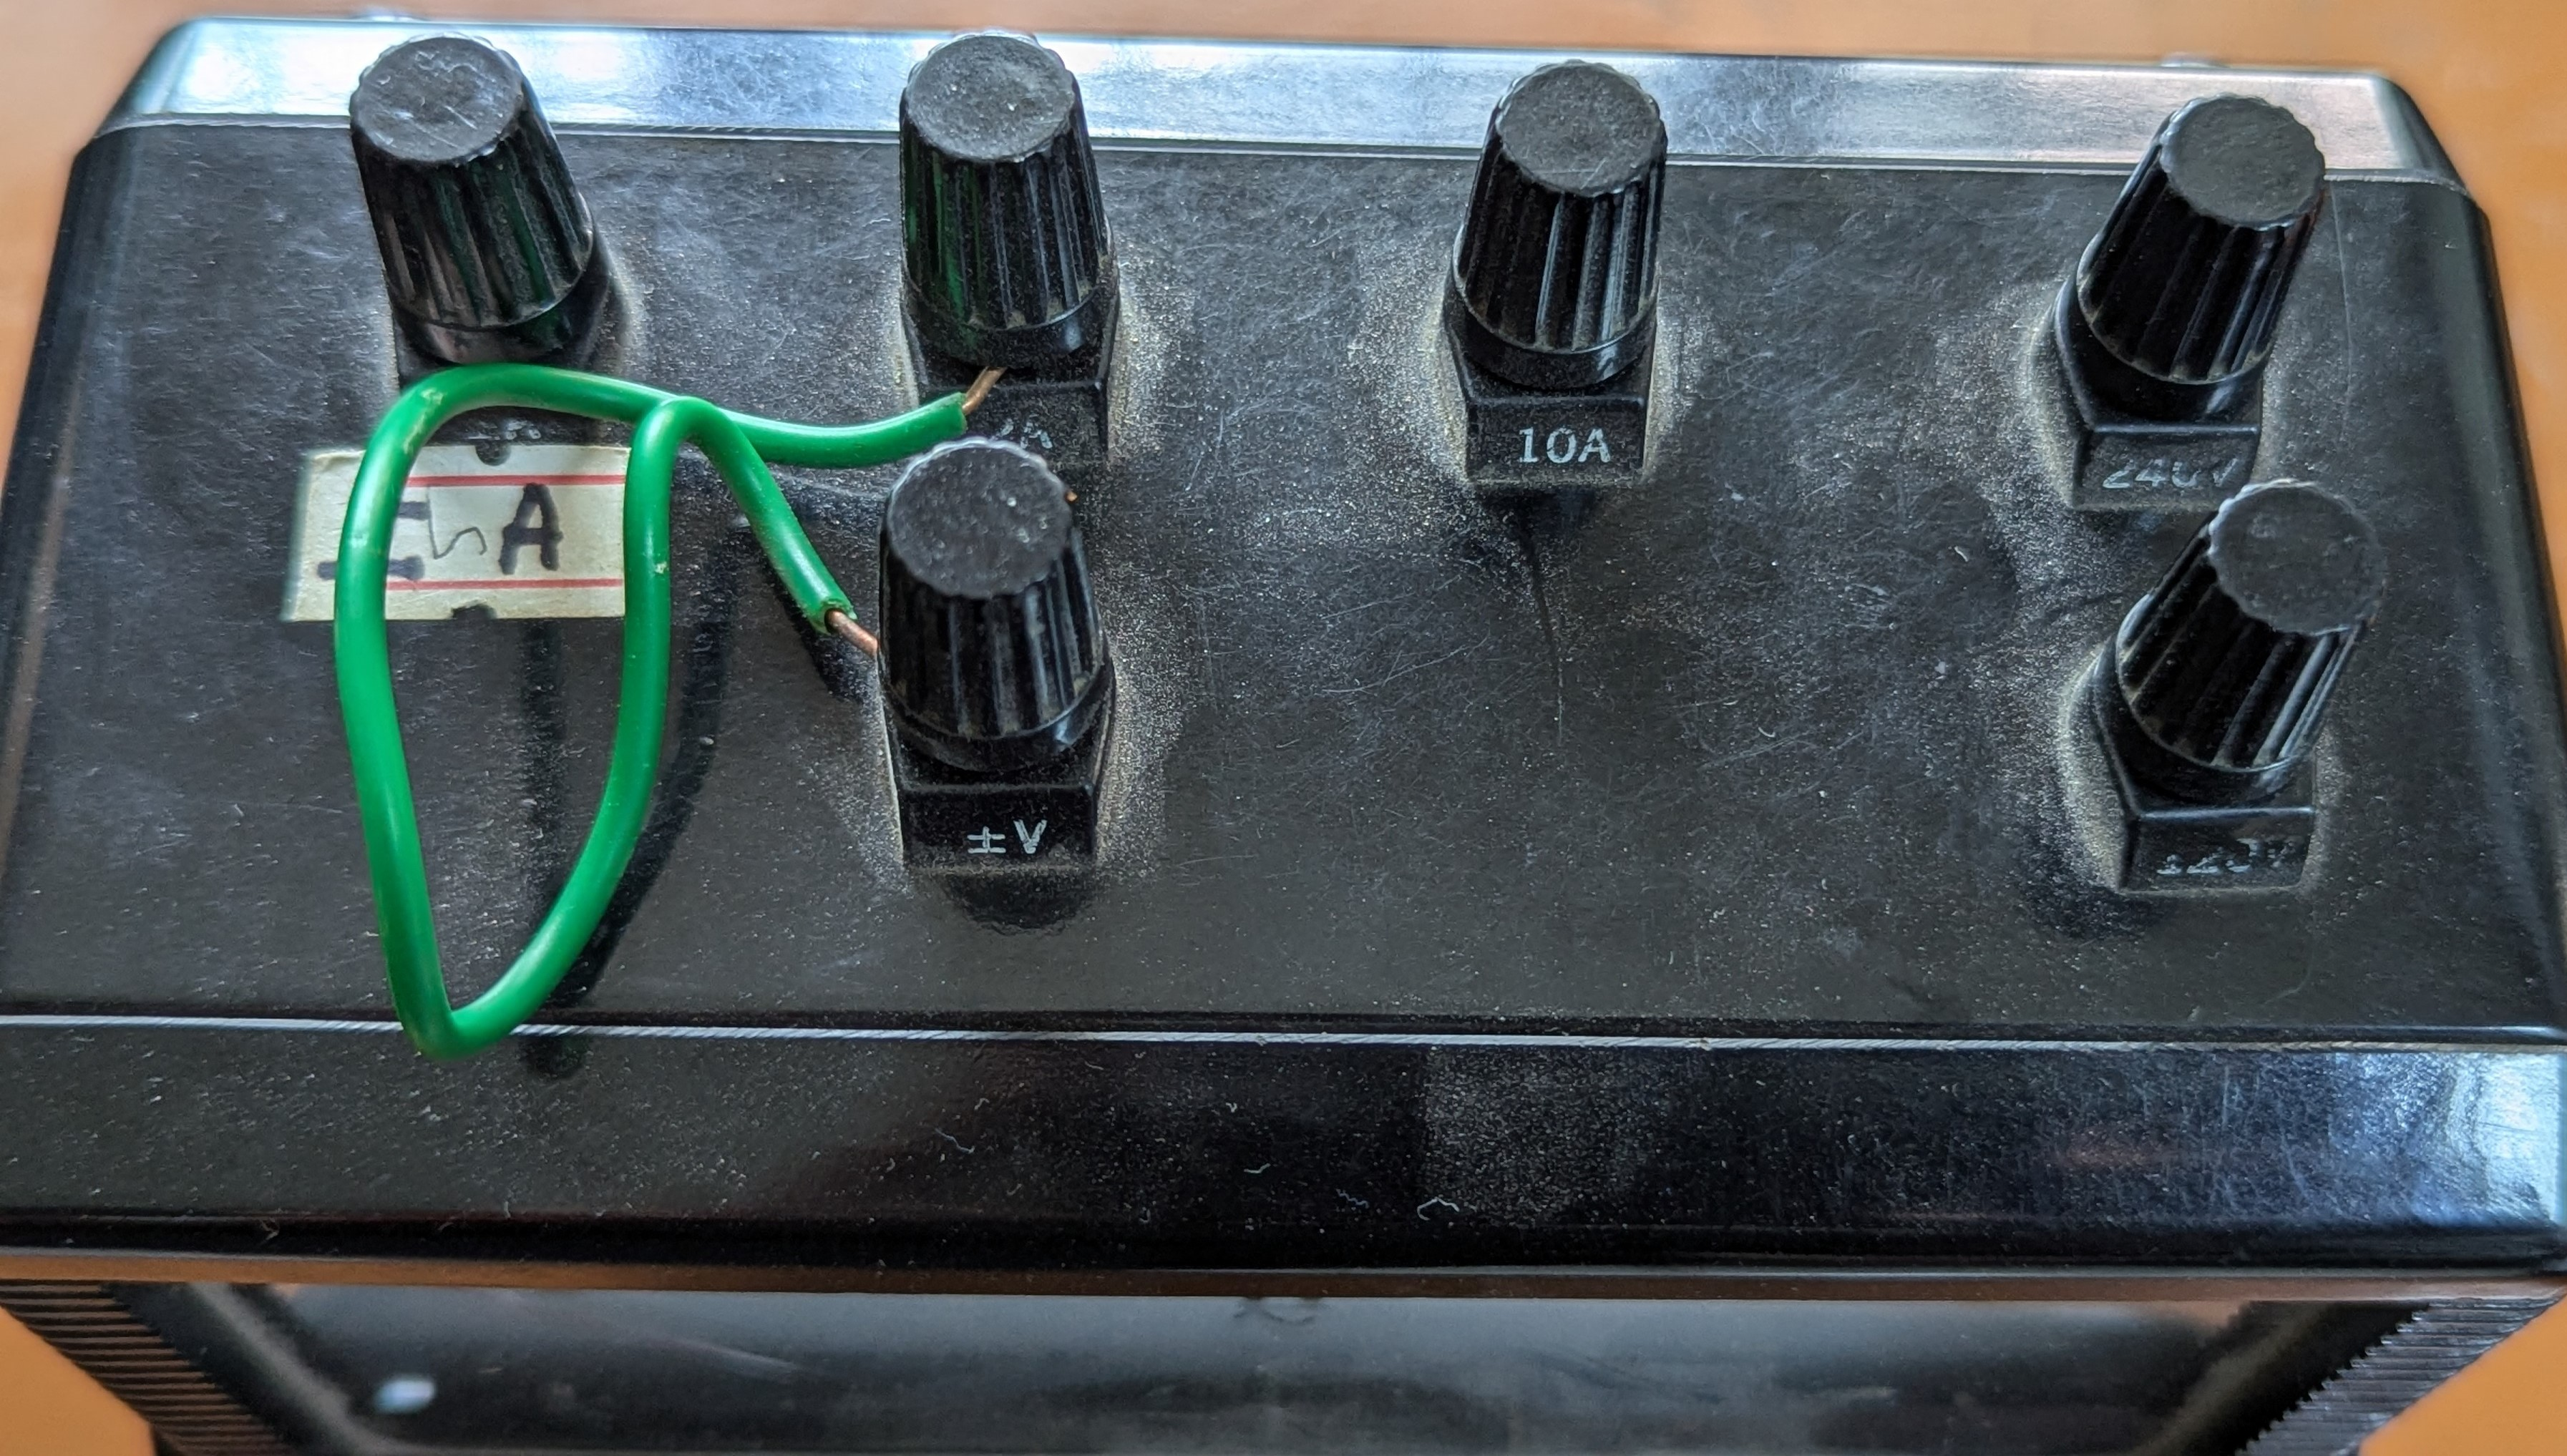
\includegraphics[width=1\linewidth]{Images/20}
			\caption{Top View}
		\end{subfigure}
		\hfill
		\begin{subfigure}[t]{0.32\textwidth}
			\centering
			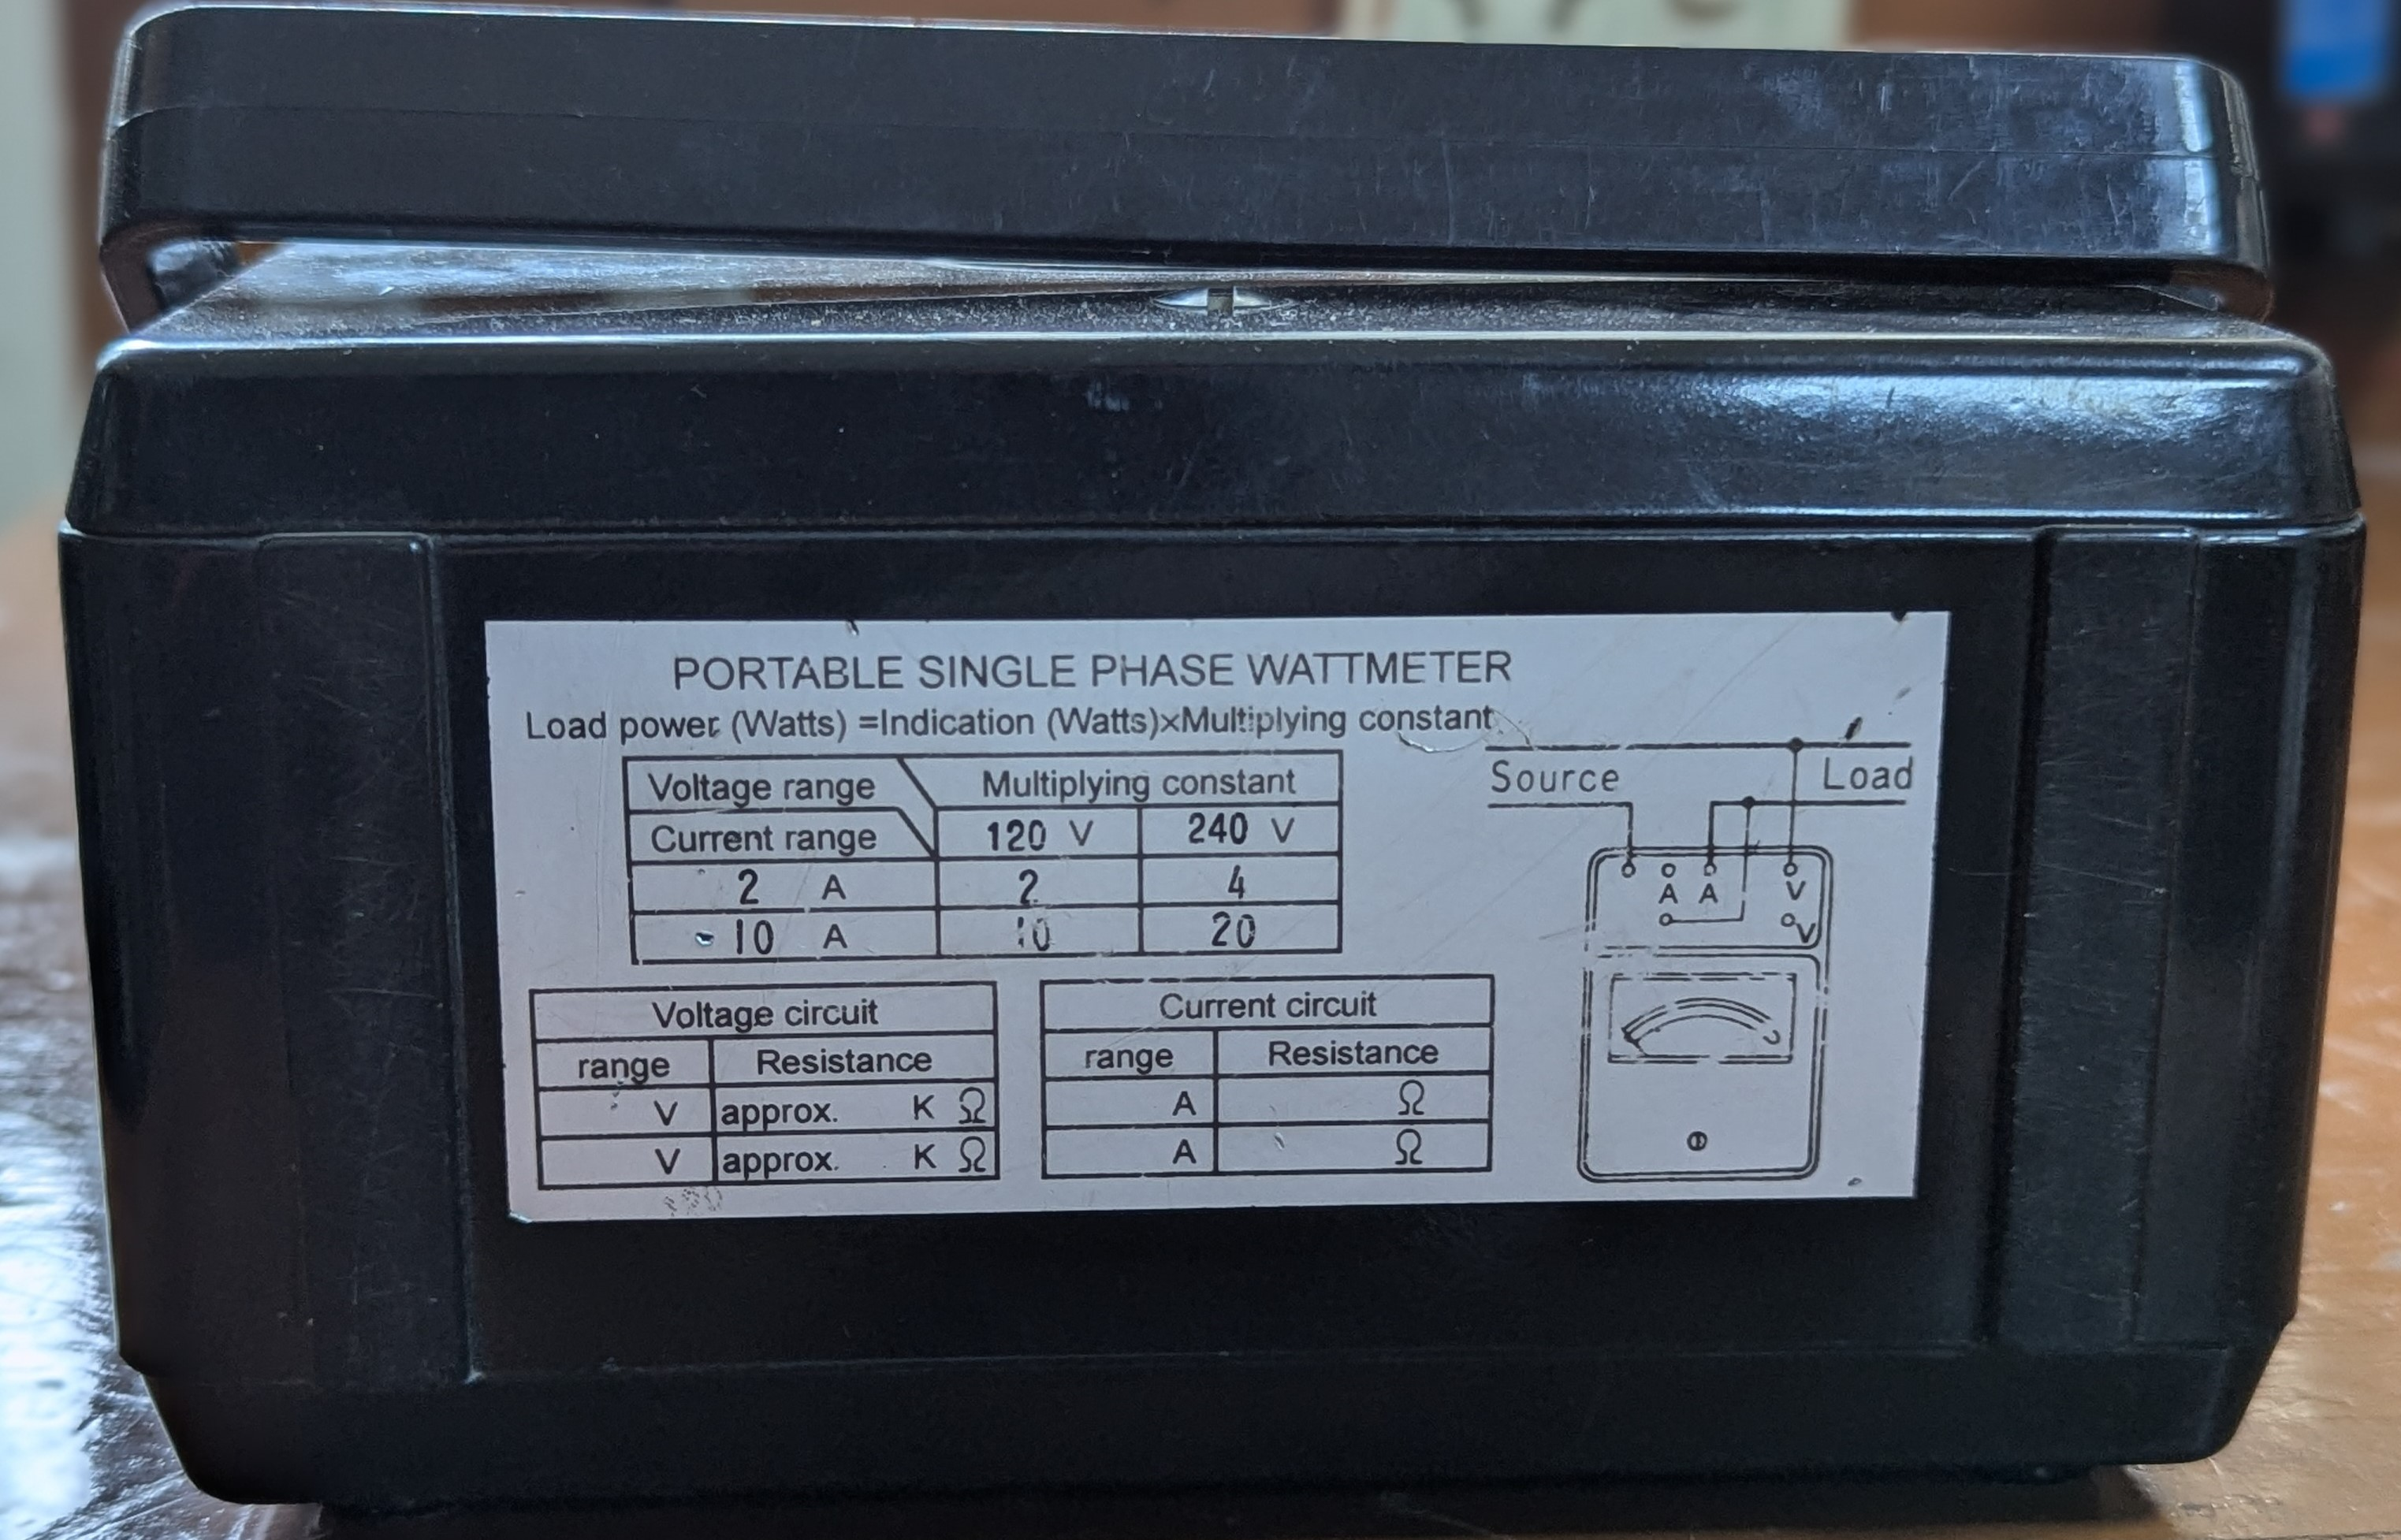
\includegraphics[width=1\linewidth]{Images/21}
			\caption{Bottom View}
		\end{subfigure}
		
		\caption{Analog Wattmeter }
		\label{fig:5}
	\end{figure}
	\newpage
	\subsection{Energy Meter}
	An energy meter, also known as an electricity meter, is a device used in a measurement laboratory to measure the amount of electrical energy consumed by a load over a specific period. These meters are essential for accurately monitoring and managing energy usage in various settings, including residential, commercial, and industrial environments.\\
	Energy meters work by continuously measuring the instantaneous voltage and current flowing through a load. The key steps in their operation are:
	\begin{itemize}
		\item \textbf{Voltage and Current Measurement:} The meter measures the instantaneous voltage and current.
		\item \textbf{Power Calculation:} The power is calculated by multiplying the instantaneous voltage by the instantaneous current.
		\item \textbf{Integration:} This power is then integrated over time to calculate the total energy consumption, usually expressed in kilowatt-hours (kWh) or megawatt-hours (MWh).
	\end{itemize}
	
	\subsubsection{Types of Energy Meters}
	\textbf{Analog Energy Meters:} Use a mechanical dial or rotating disk to measure energy consumption. These meters are less common today but are still used in some applications. \\
	\textbf{Digital Energy Meters:} Utilize electronic sensors and digital displays to provide precise measurements of energy consumption. They often include features such as remote reading capabilities and real-time monitoring.
	

	
	\begin{figure}[H]
		\centering
		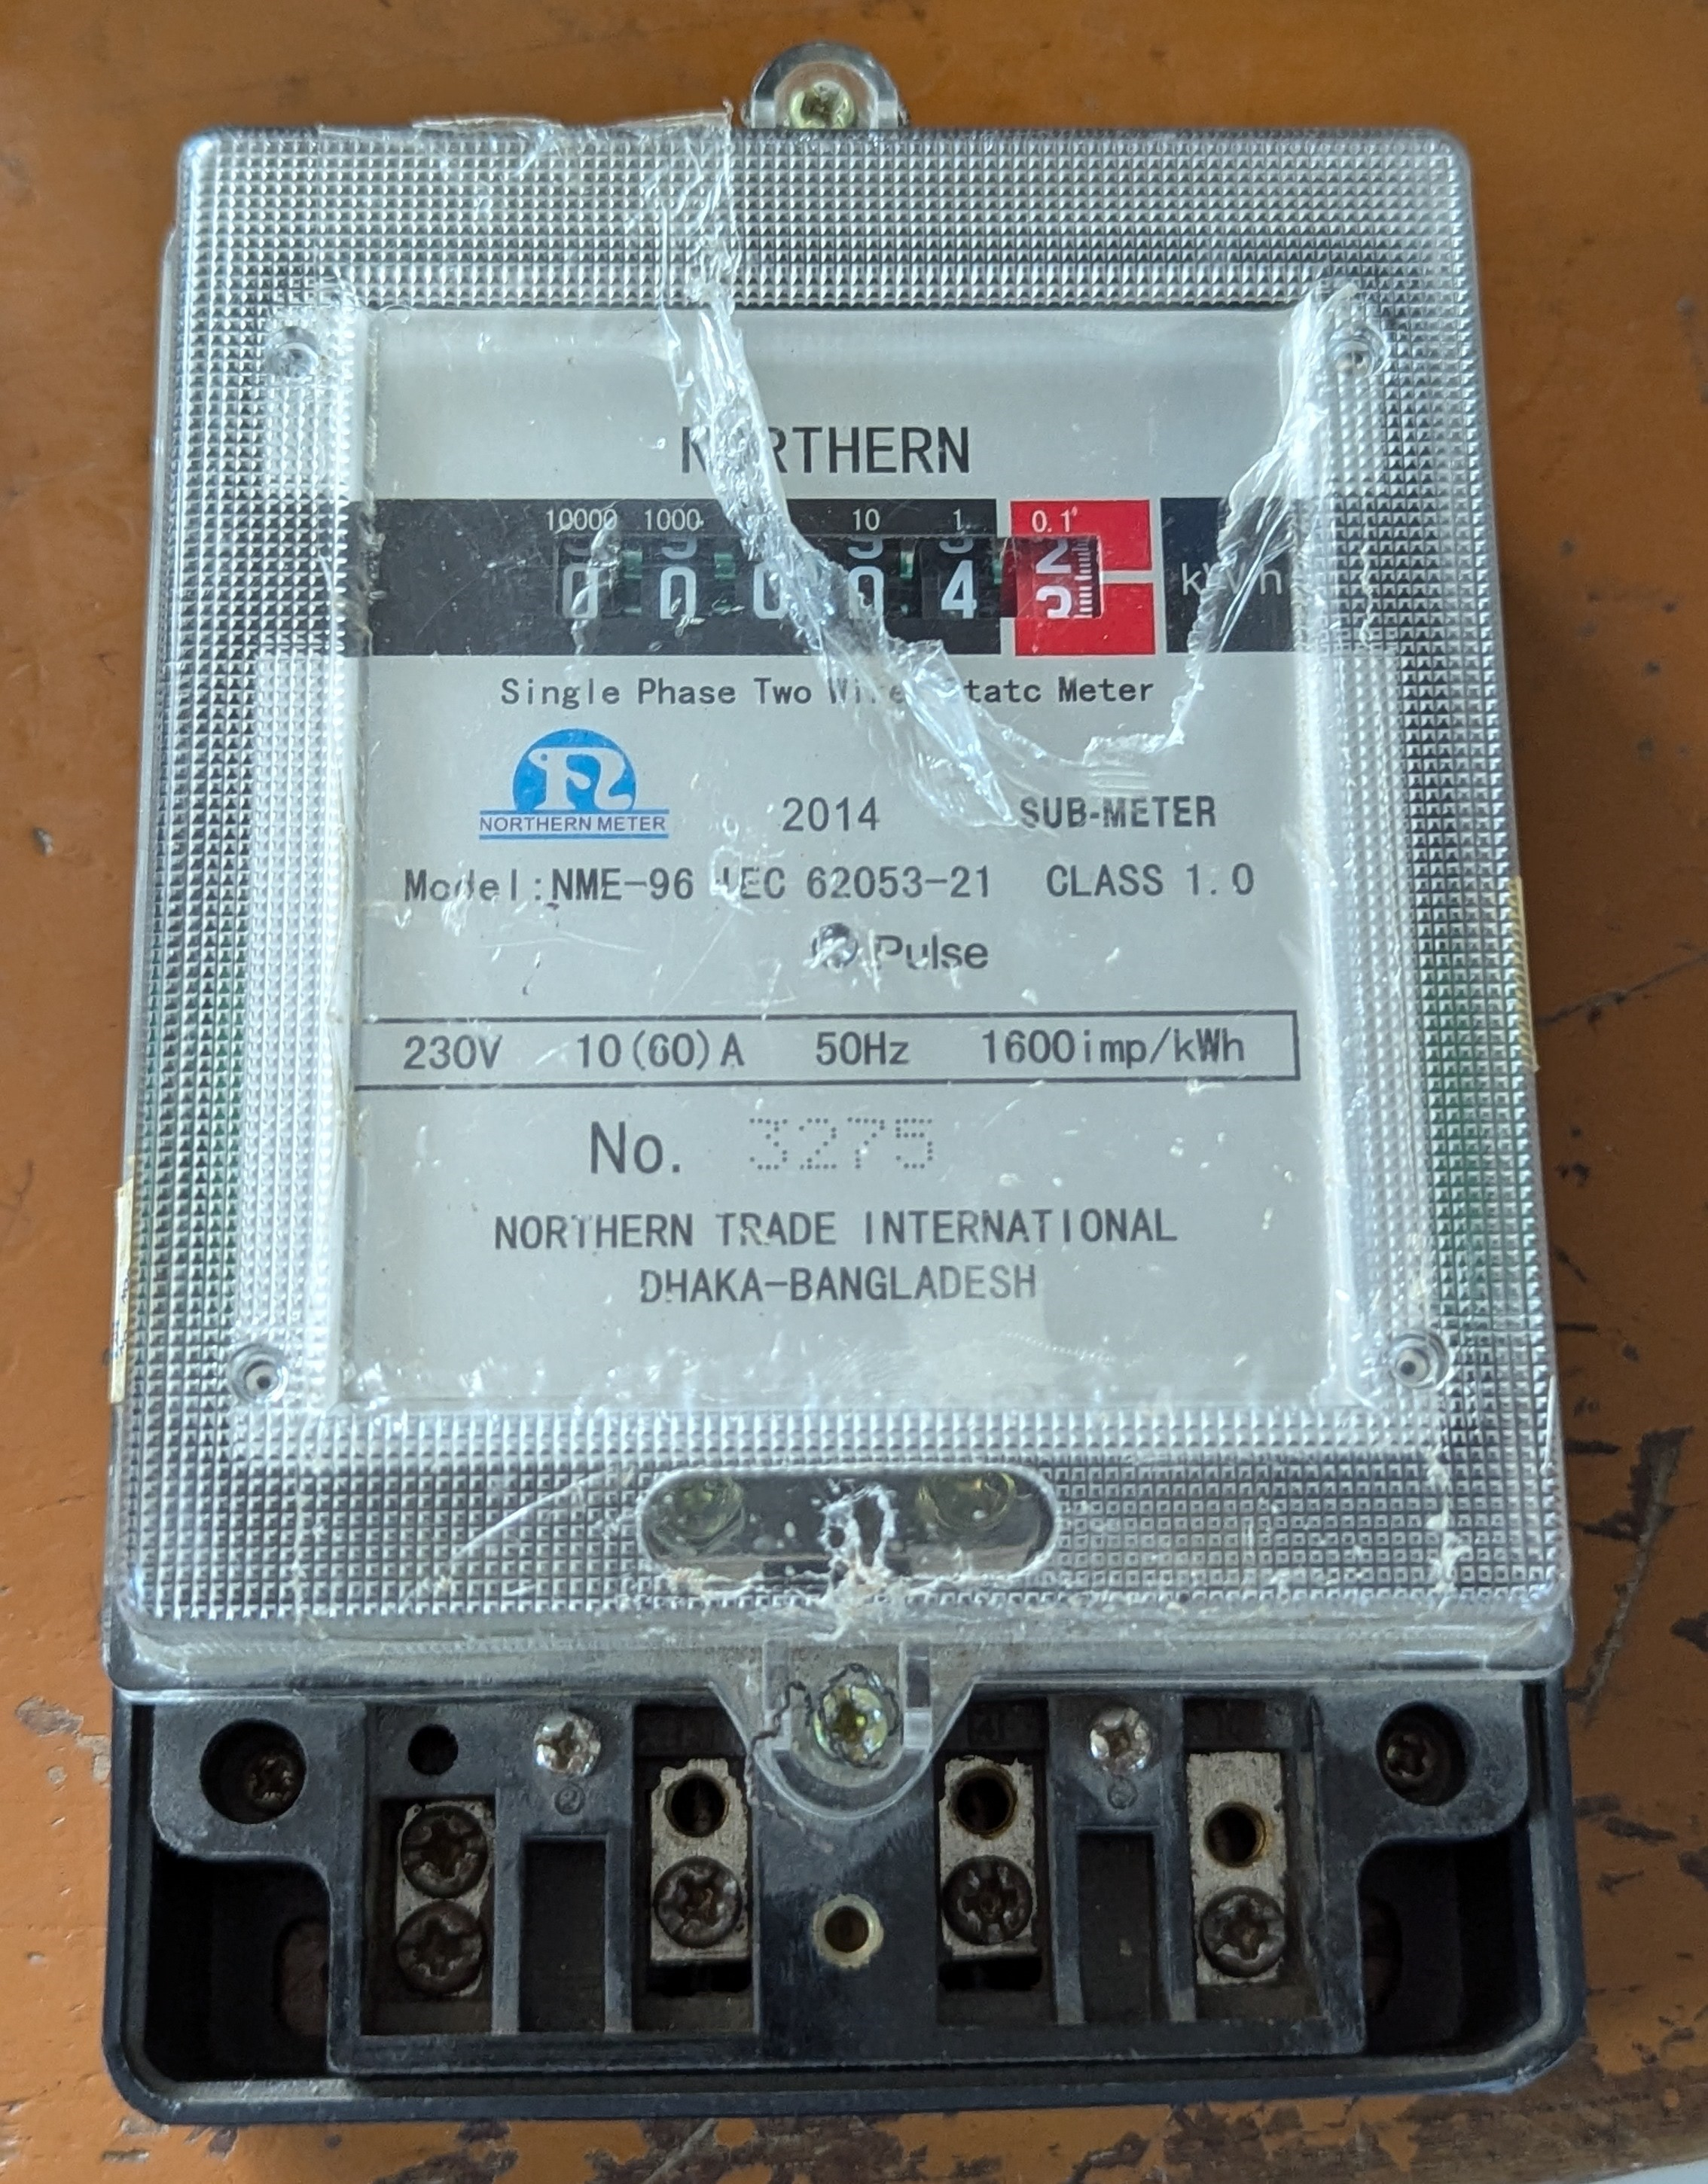
\includegraphics[width=0.45\linewidth]{Images/17}
		\caption{Analog Energy Meter}
		\label{fig:4}
	\end{figure}
	\newpage
	\subsection{Transformer}
	A transformer is an electrical device used to transfer electrical energy between two or more circuits through electromagnetic induction. It consists of two or more wire coils (windings) wrapped around a common core. Transformers are used to step up or step down voltage levels and to isolate different parts of an electrical system.\\
	\textbf{Current Transformer (CT):} Used to measure the current in a circuit. It produces a secondary current that is proportional to the primary current, allowing for accurate measurement and monitoring. \\
	\textbf{Potential Transformer (PT):} Also known as a Voltage Transformer, it is used to measure voltage in a circuit. It steps down high voltage to a lower, manageable level for measurement and monitoring.
	
	\subsubsection{Working Principle}
	Both types of transformers operate on the principle of electromagnetic induction:
	\begin{itemize}
		\item \textbf{Current Transformer (CT):} The primary winding is connected in series with the circuit carrying the current. The current flowing through the primary winding induces a proportional current in the secondary winding, which can be measured using standard instrumentation.
		\item \textbf{Potential Transformer (PT):} The primary winding is connected across the high-voltage circuit. The voltage induces a proportional voltage in the secondary winding, which is reduced to a safer, lower voltage suitable for measurement by standard instruments.
	\end{itemize}
	
	Transformers are essential for accurate measurement, protection, and control in electrical systems.
	
	\subsubsection{Current Transformer (CT)}
			\begin{figure}[H]
		\centering
		\begin{subfigure}[t]{0.49\textwidth}
			\centering
			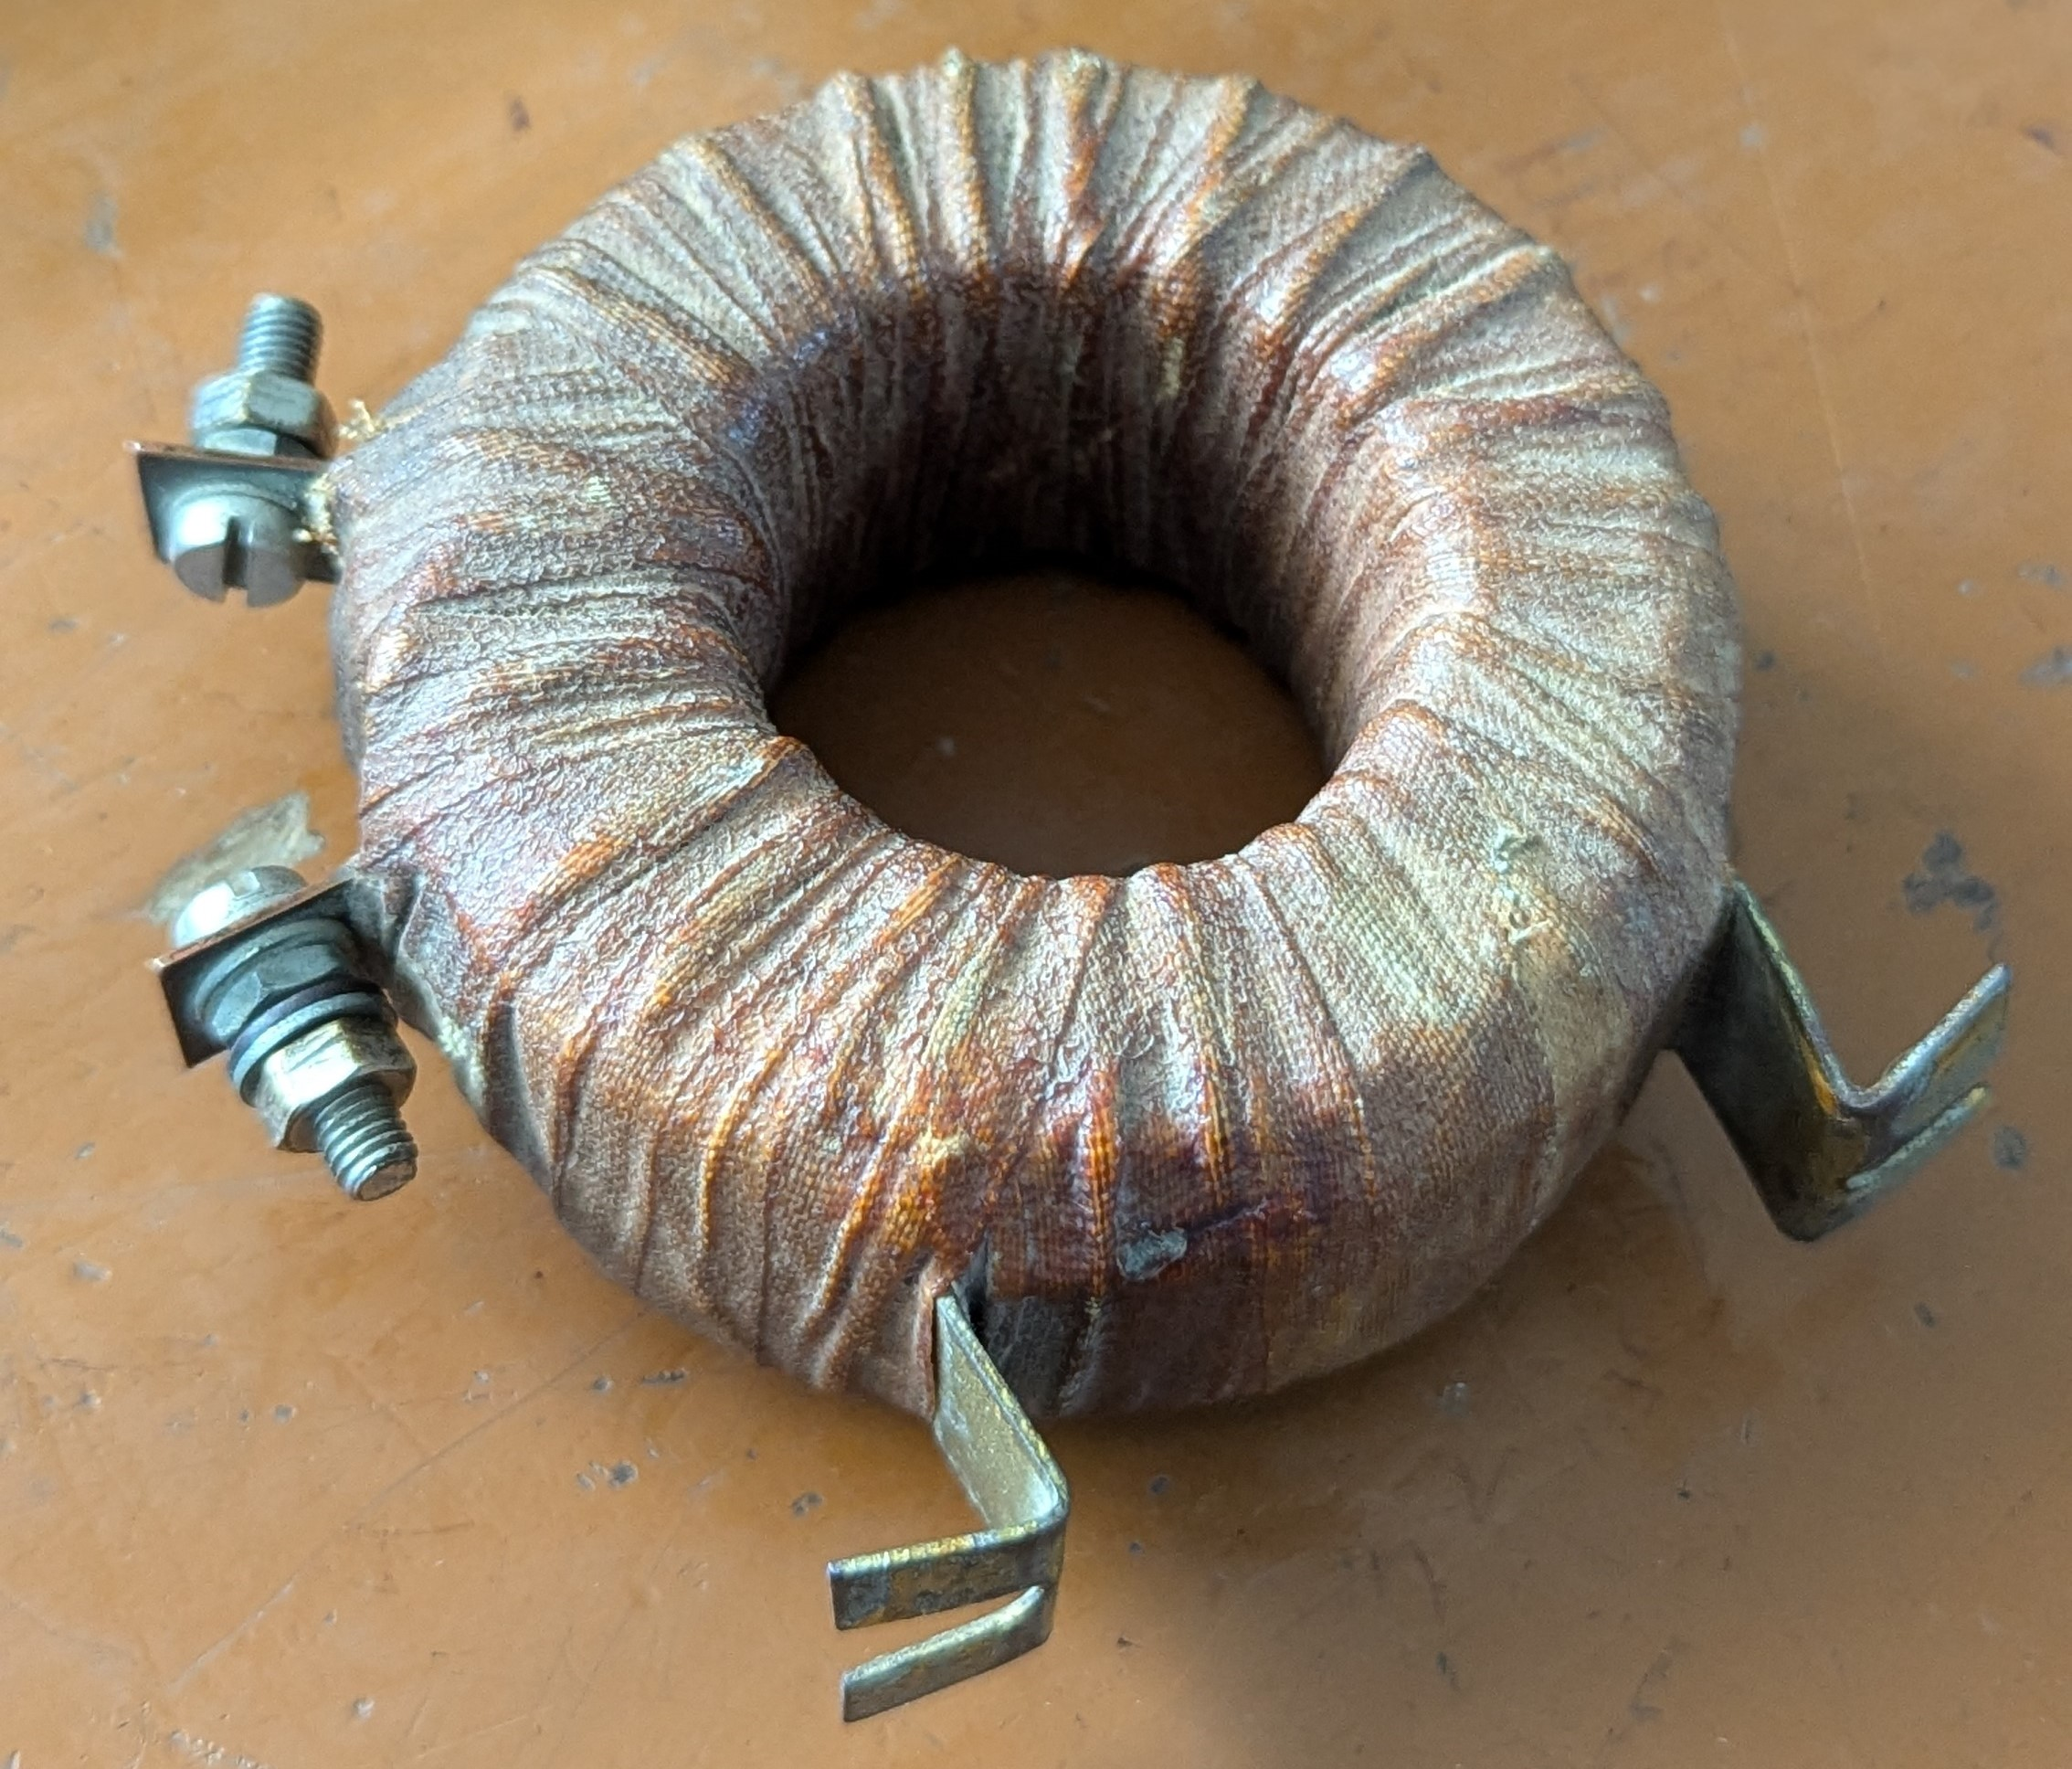
\includegraphics[width=0.9\linewidth]{Images/25}
			\caption{}
		\end{subfigure}
		\hfill
		\begin{subfigure}[t]{0.49\textwidth}
			\centering
			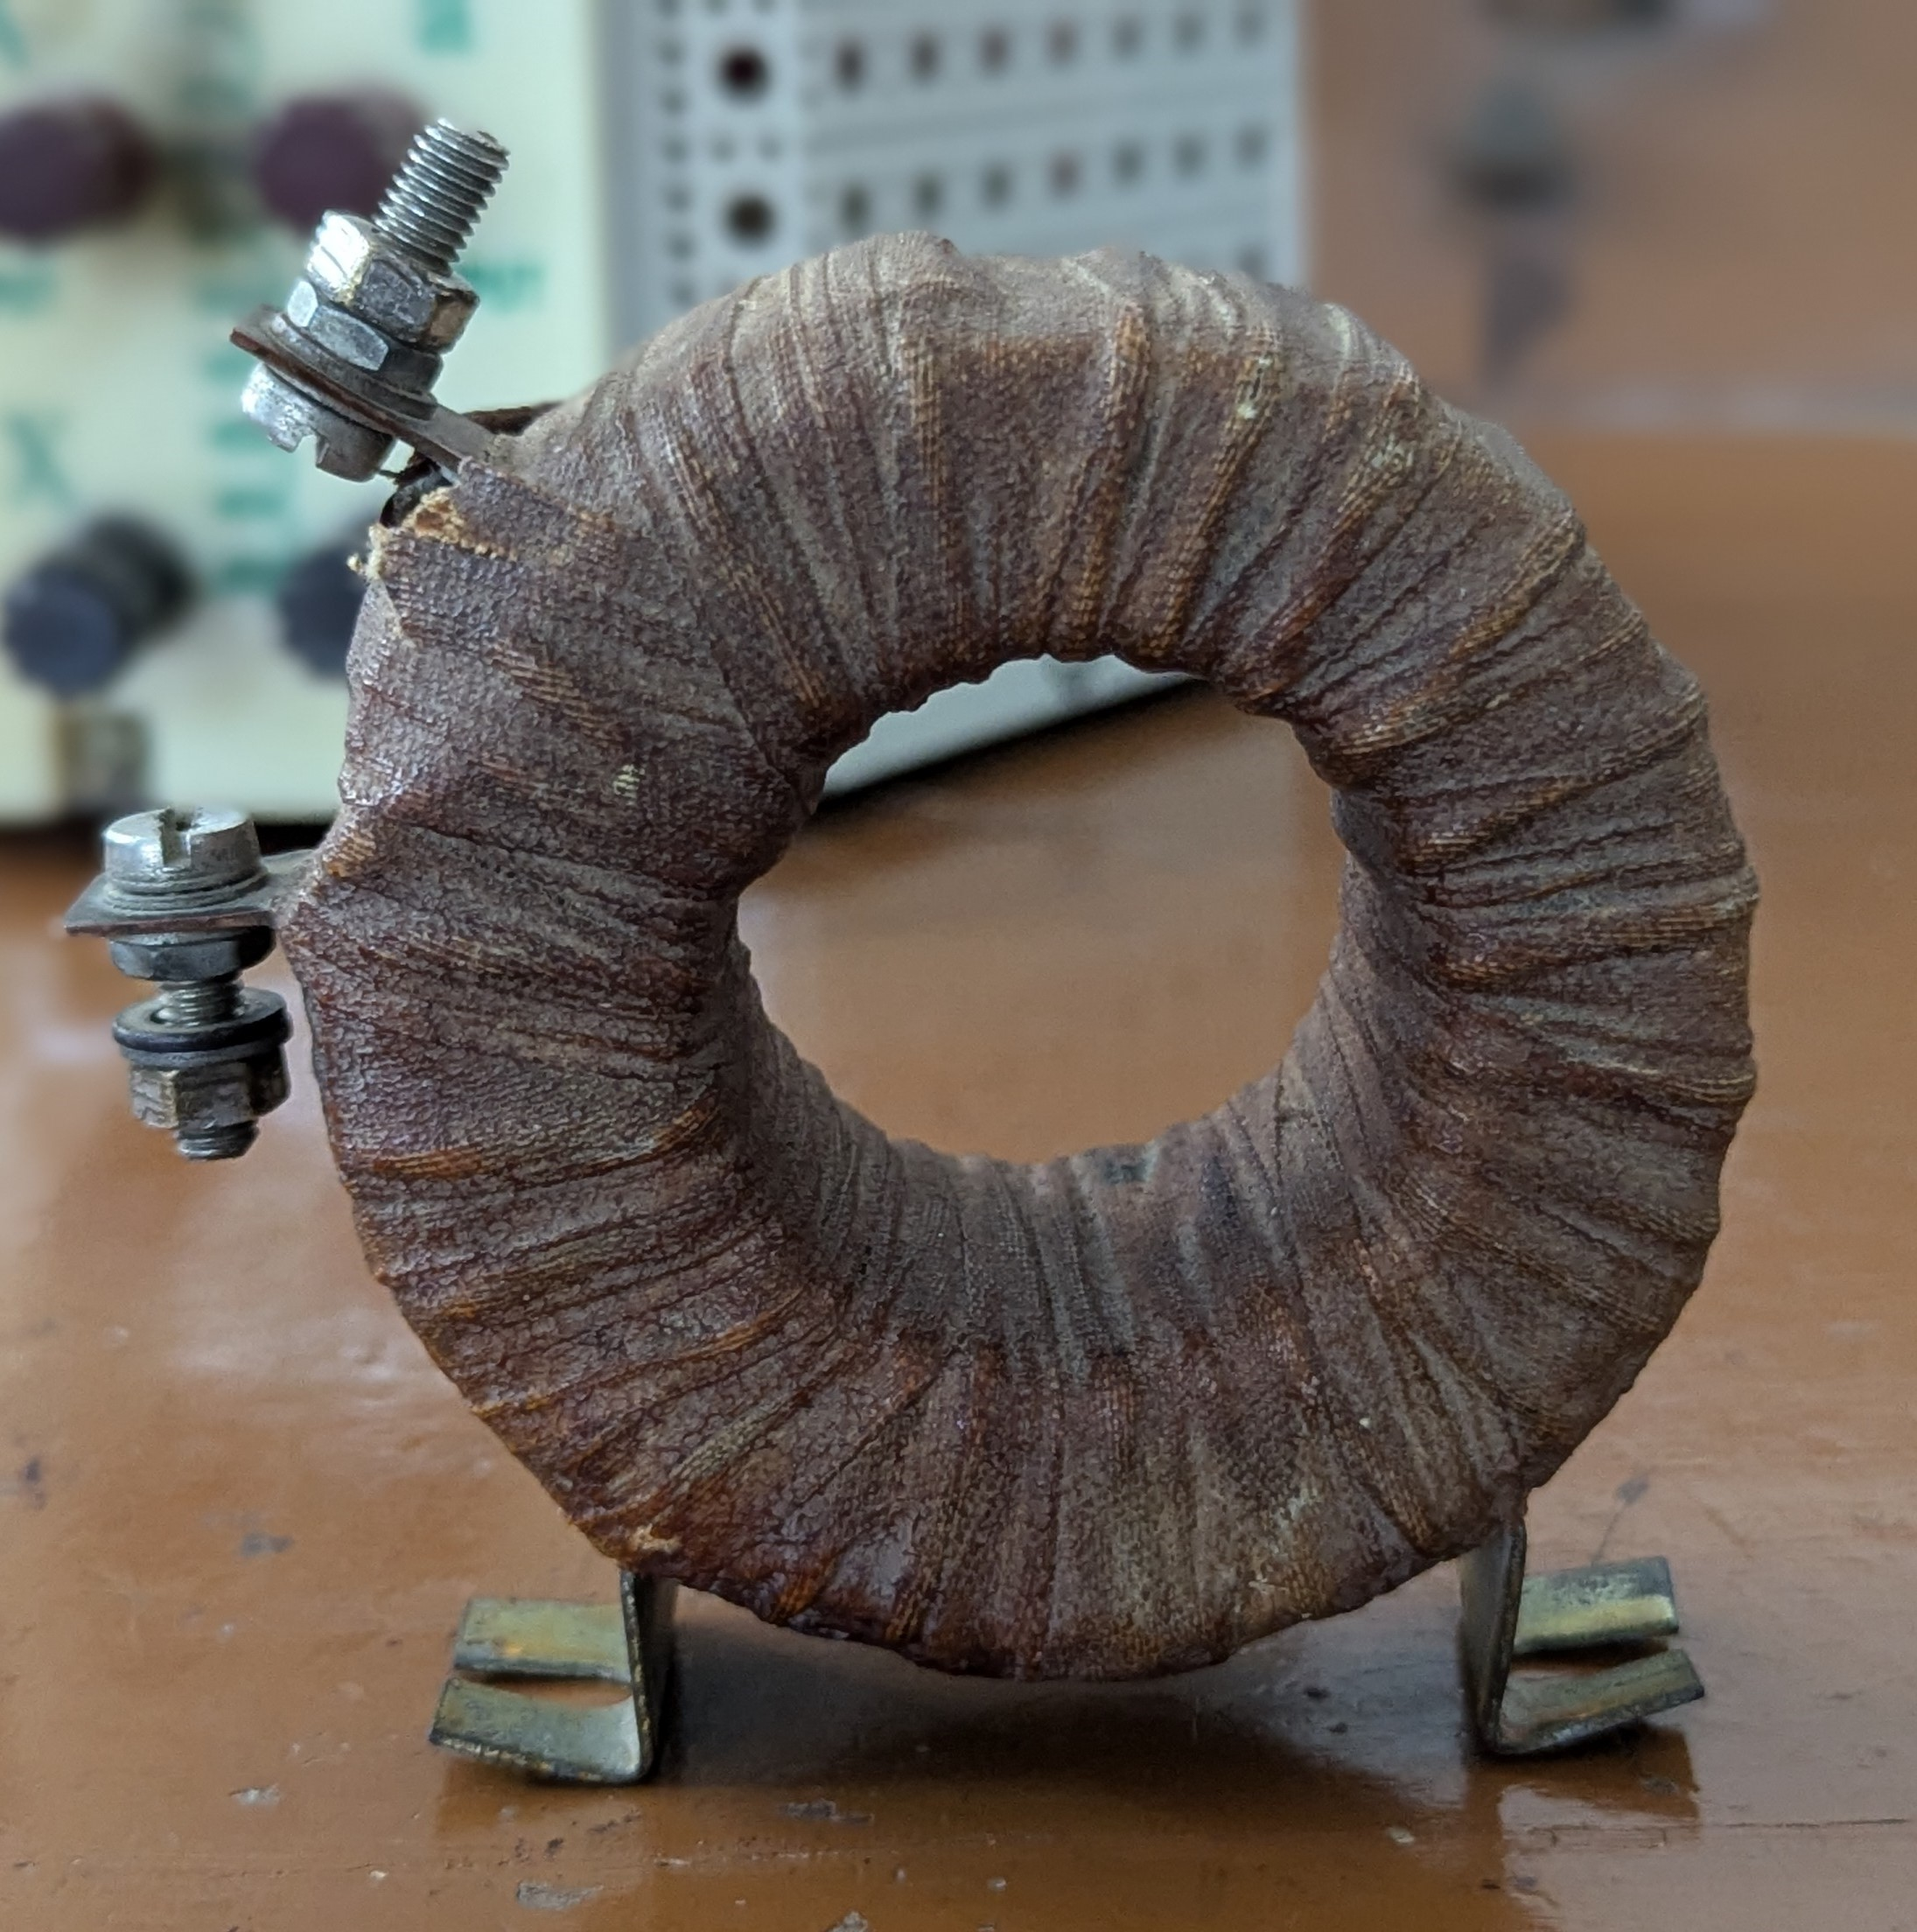
\includegraphics[width=0.9\linewidth]{Images/26}
			\caption{}
		\end{subfigure}
		
		\caption{Current Transformer (CT)}
		\label{fig:5}
	\end{figure}
	
	
	\subsubsection{Potential Transformer (PT)}
			\begin{figure}[H]
		\centering
		\begin{subfigure}[t]{0.49\textwidth}
			\centering
			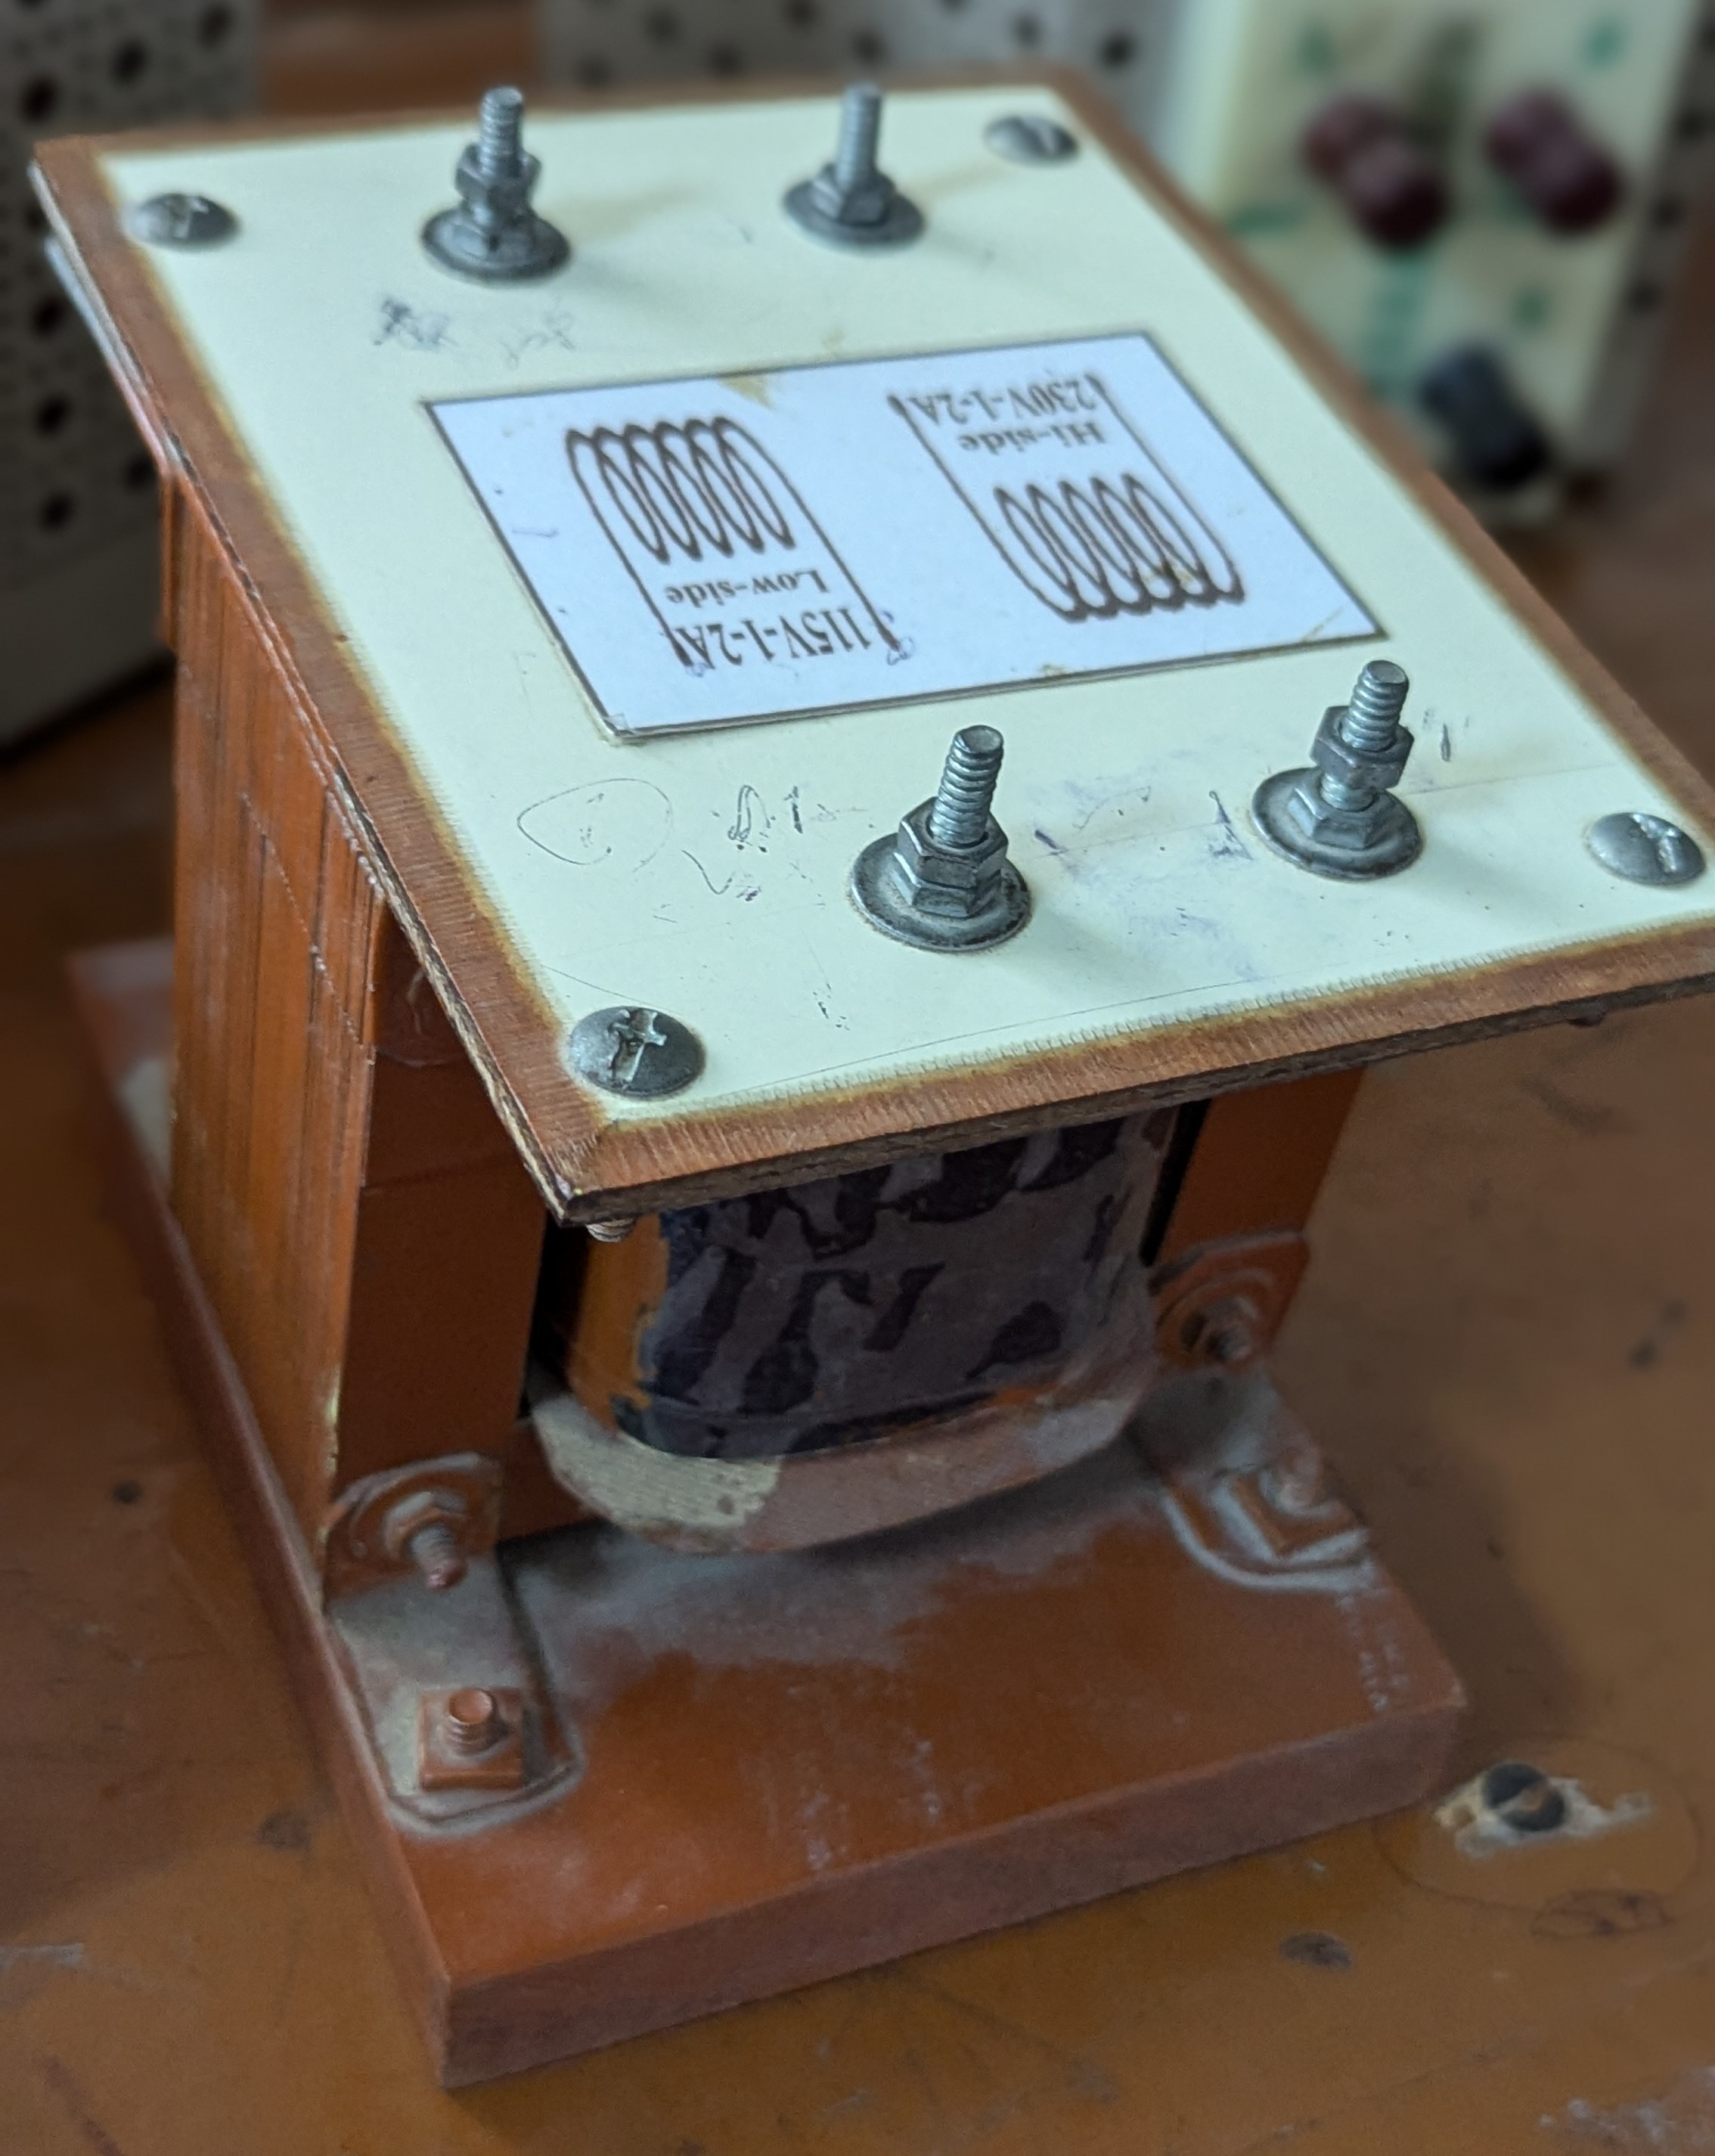
\includegraphics[width=0.7\linewidth]{Images/22}
			\caption{}
		\end{subfigure}
		\hfill
		\begin{subfigure}[t]{0.49\textwidth}
			\centering
			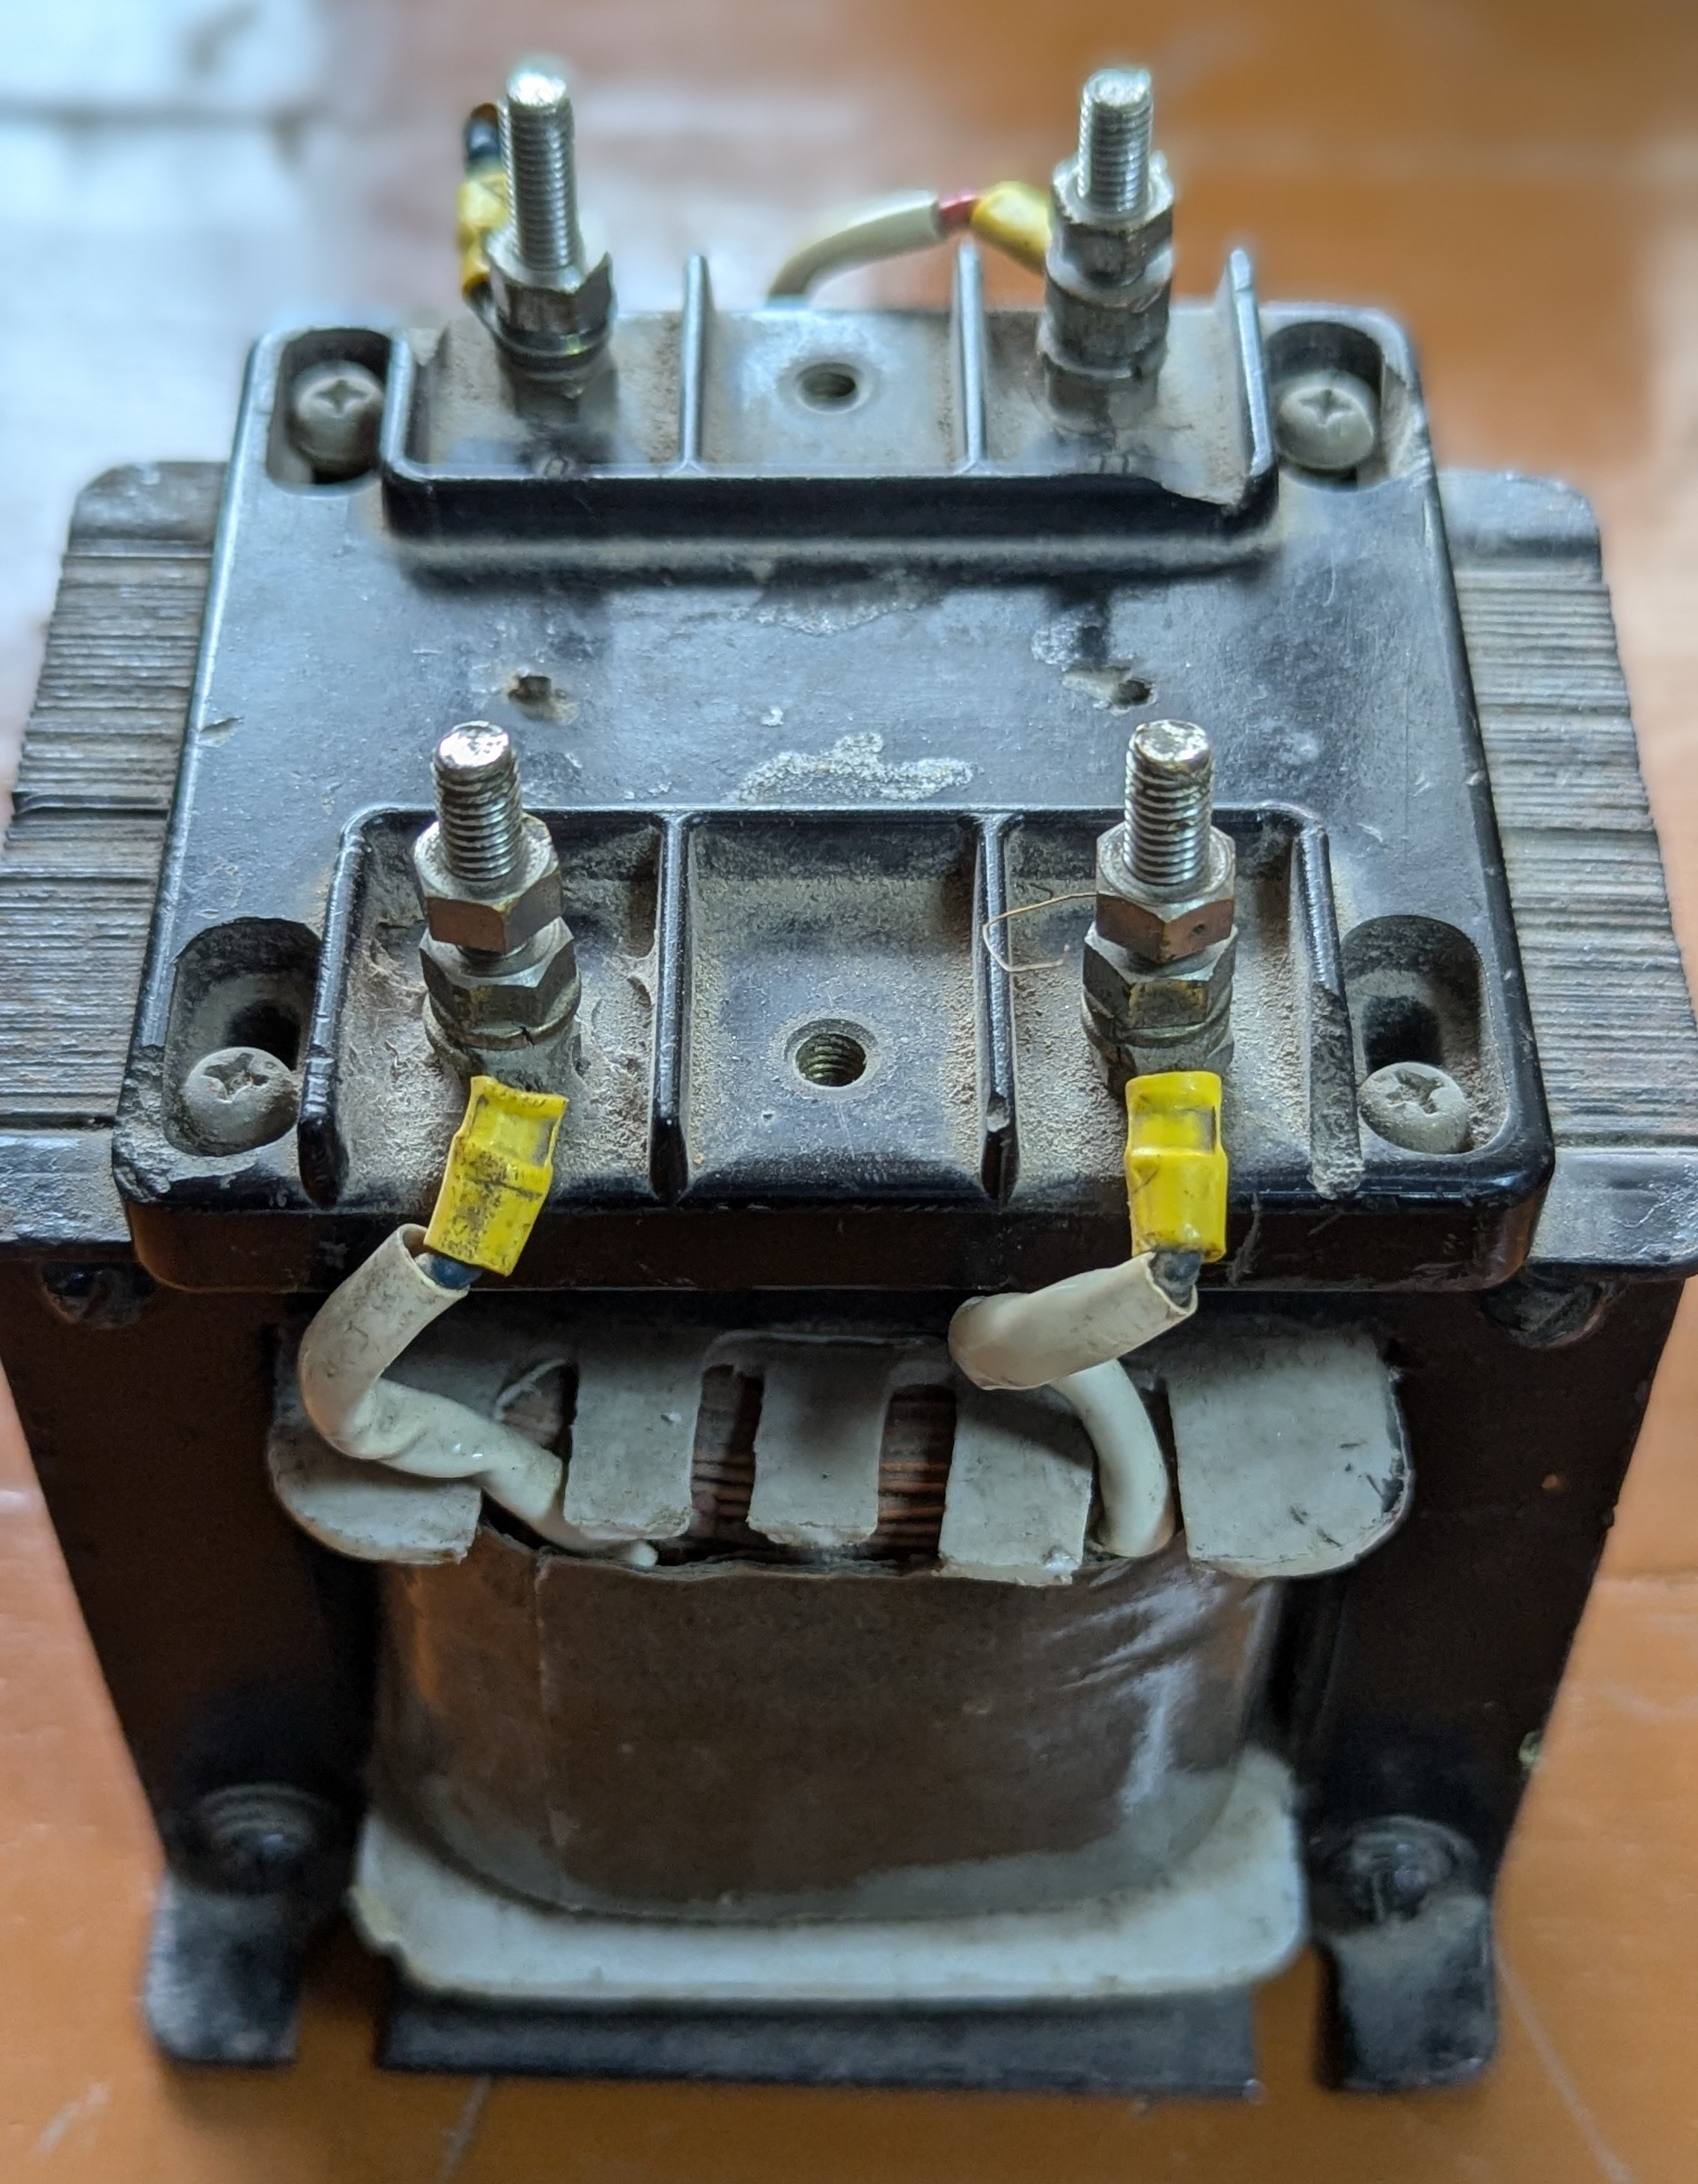
\includegraphics[width=0.7\linewidth]{Images/24}
			\caption{}
		\end{subfigure}
		
		\caption{Potential Transformer(PT) }
		\label{fig:5}
	\end{figure}
\subsection{Laboratory DC Power Supply}
A laboratory DC power supply is an electronic device used to provide a stable and adjustable direct current (DC) voltage to various electronic circuits and components. It is essential for powering experiments, testing circuits, and providing precise voltage and current for accurate measurements.
The laboratory DC power supply operates on the principle of converting alternating current (AC) from the mains supply into a stable DC output.The laboratory DC power supply is crucial for providing reliable and adjustable power to electronic devices and for conducting precise electrical experiments.

			\begin{figure}[H]
		\centering
		\scalebox{1}{
		\begin{subfigure}[t]{0.49\textwidth}
			\centering
			
			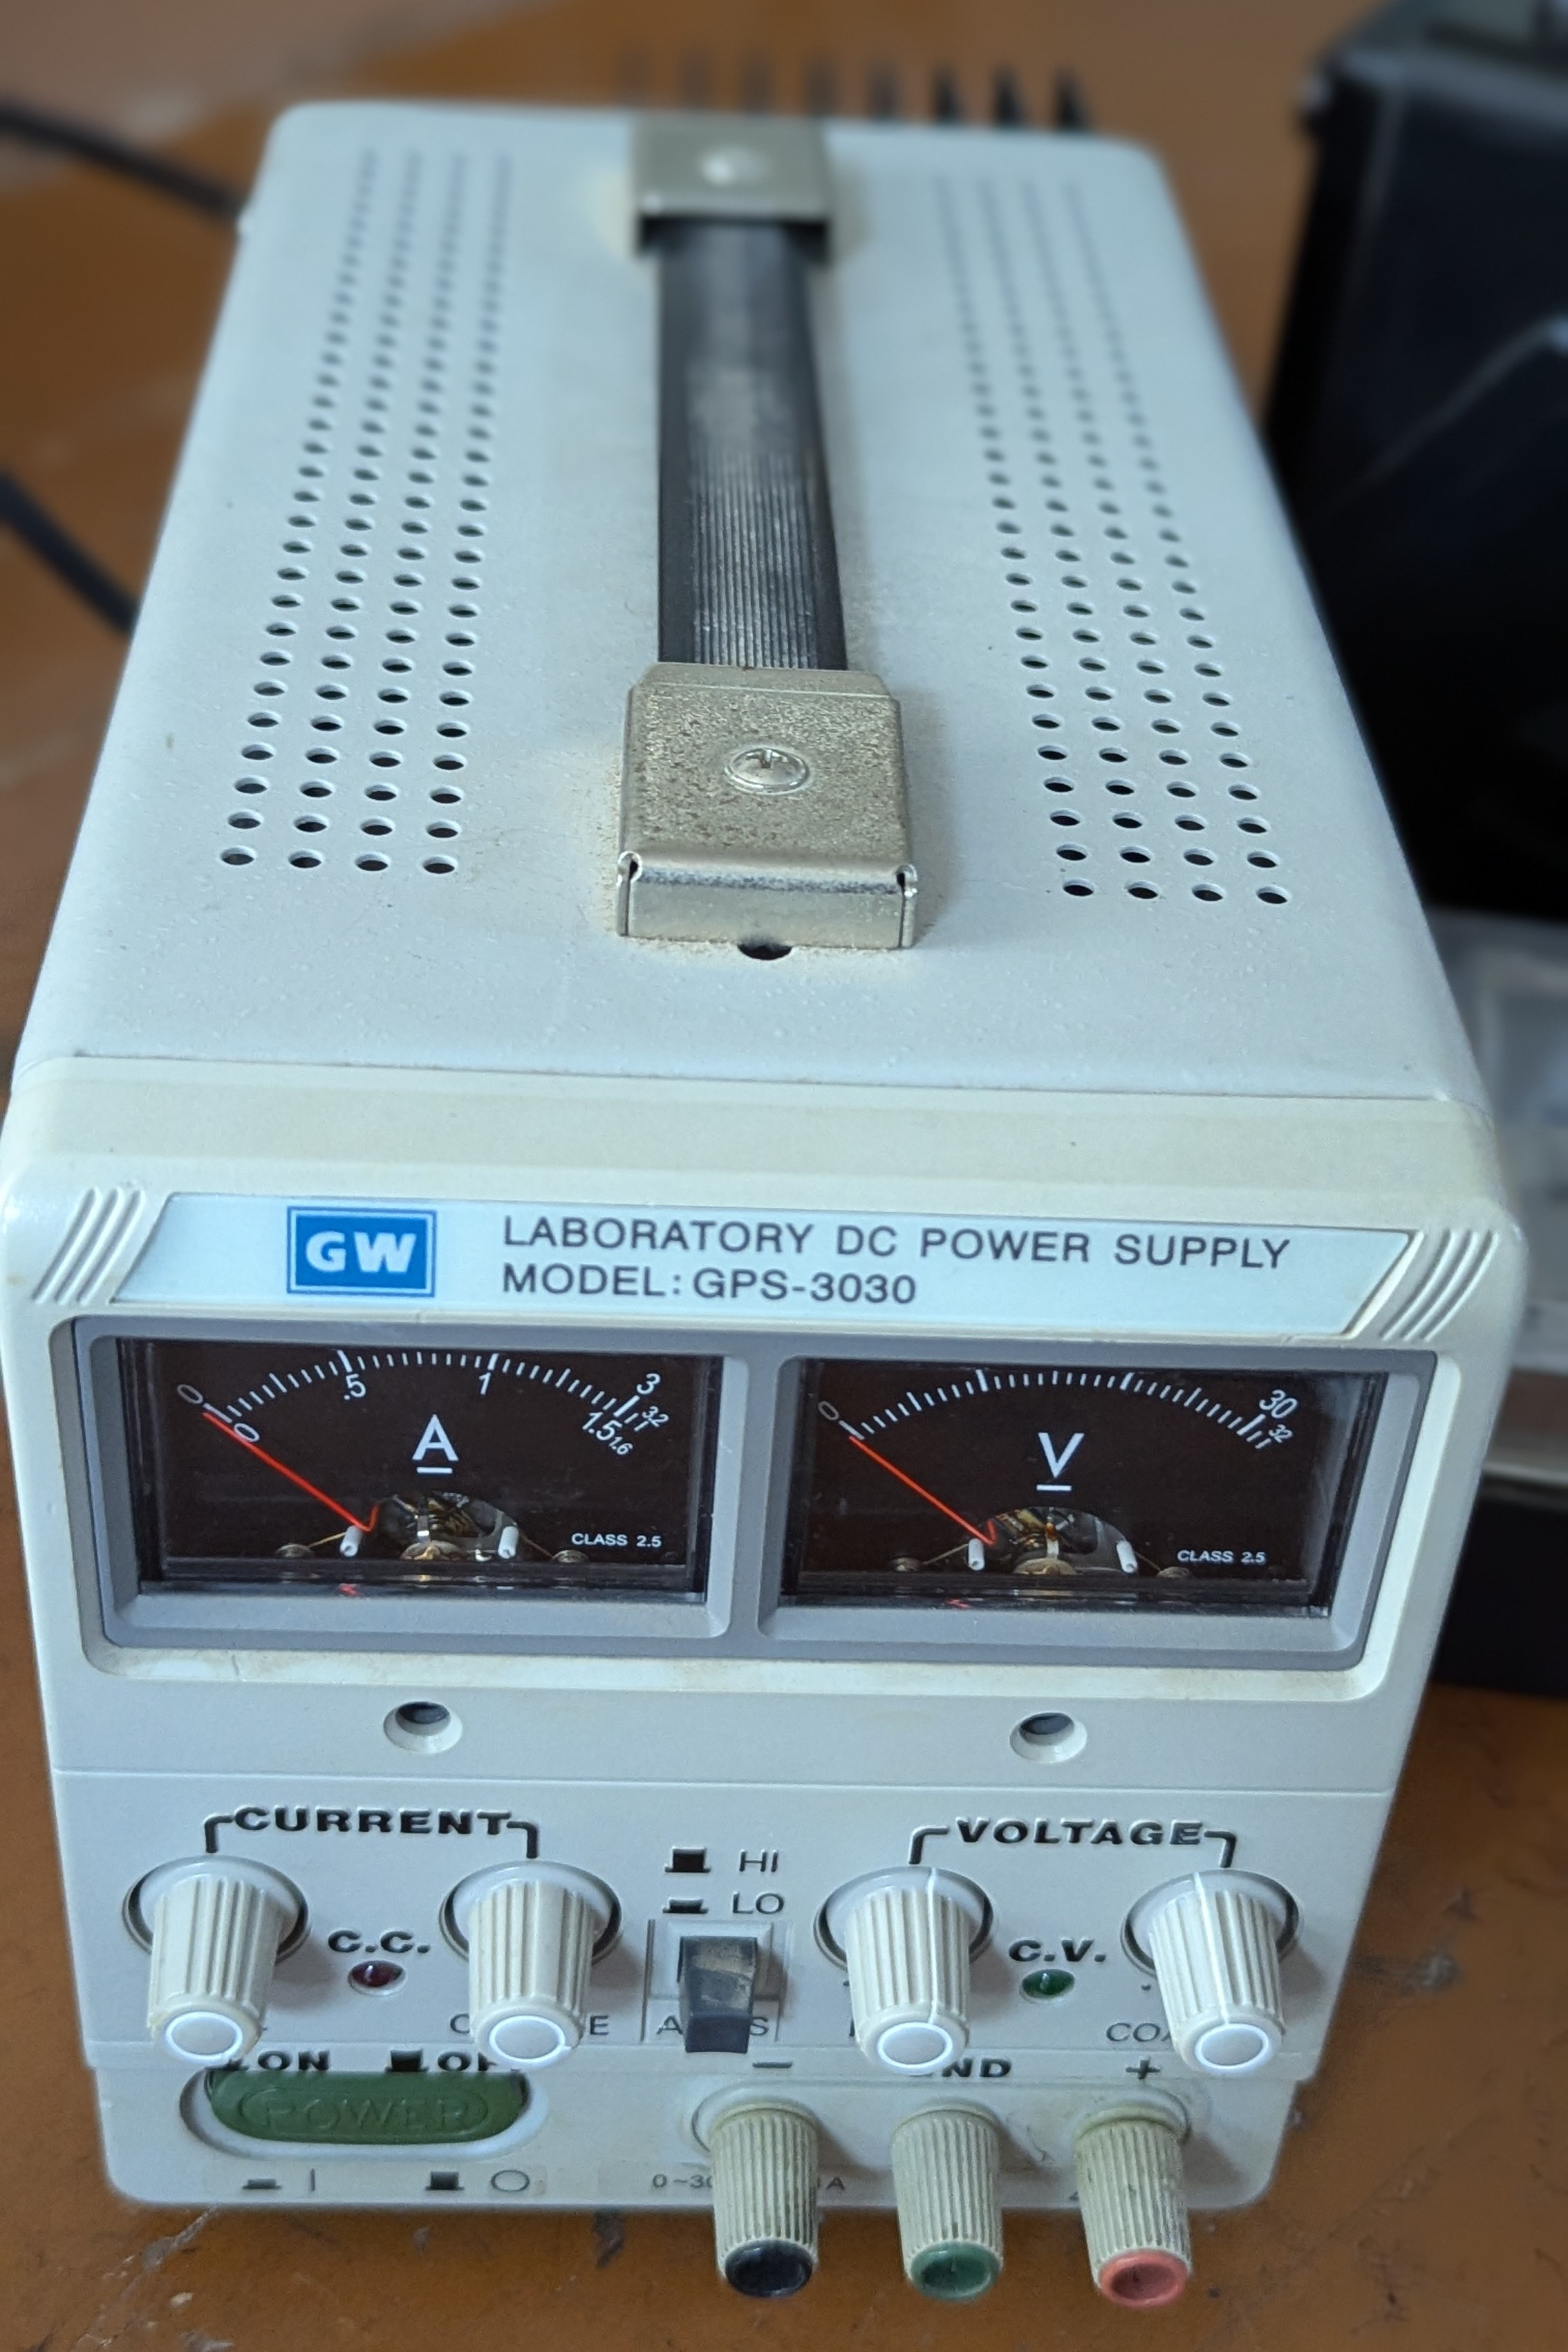
\includegraphics[width=0.7\linewidth]{Images/27}
			\caption{Front View}
		\end{subfigure}
		\hfill
		\begin{subfigure}[t]{0.49\textwidth}
			\centering
			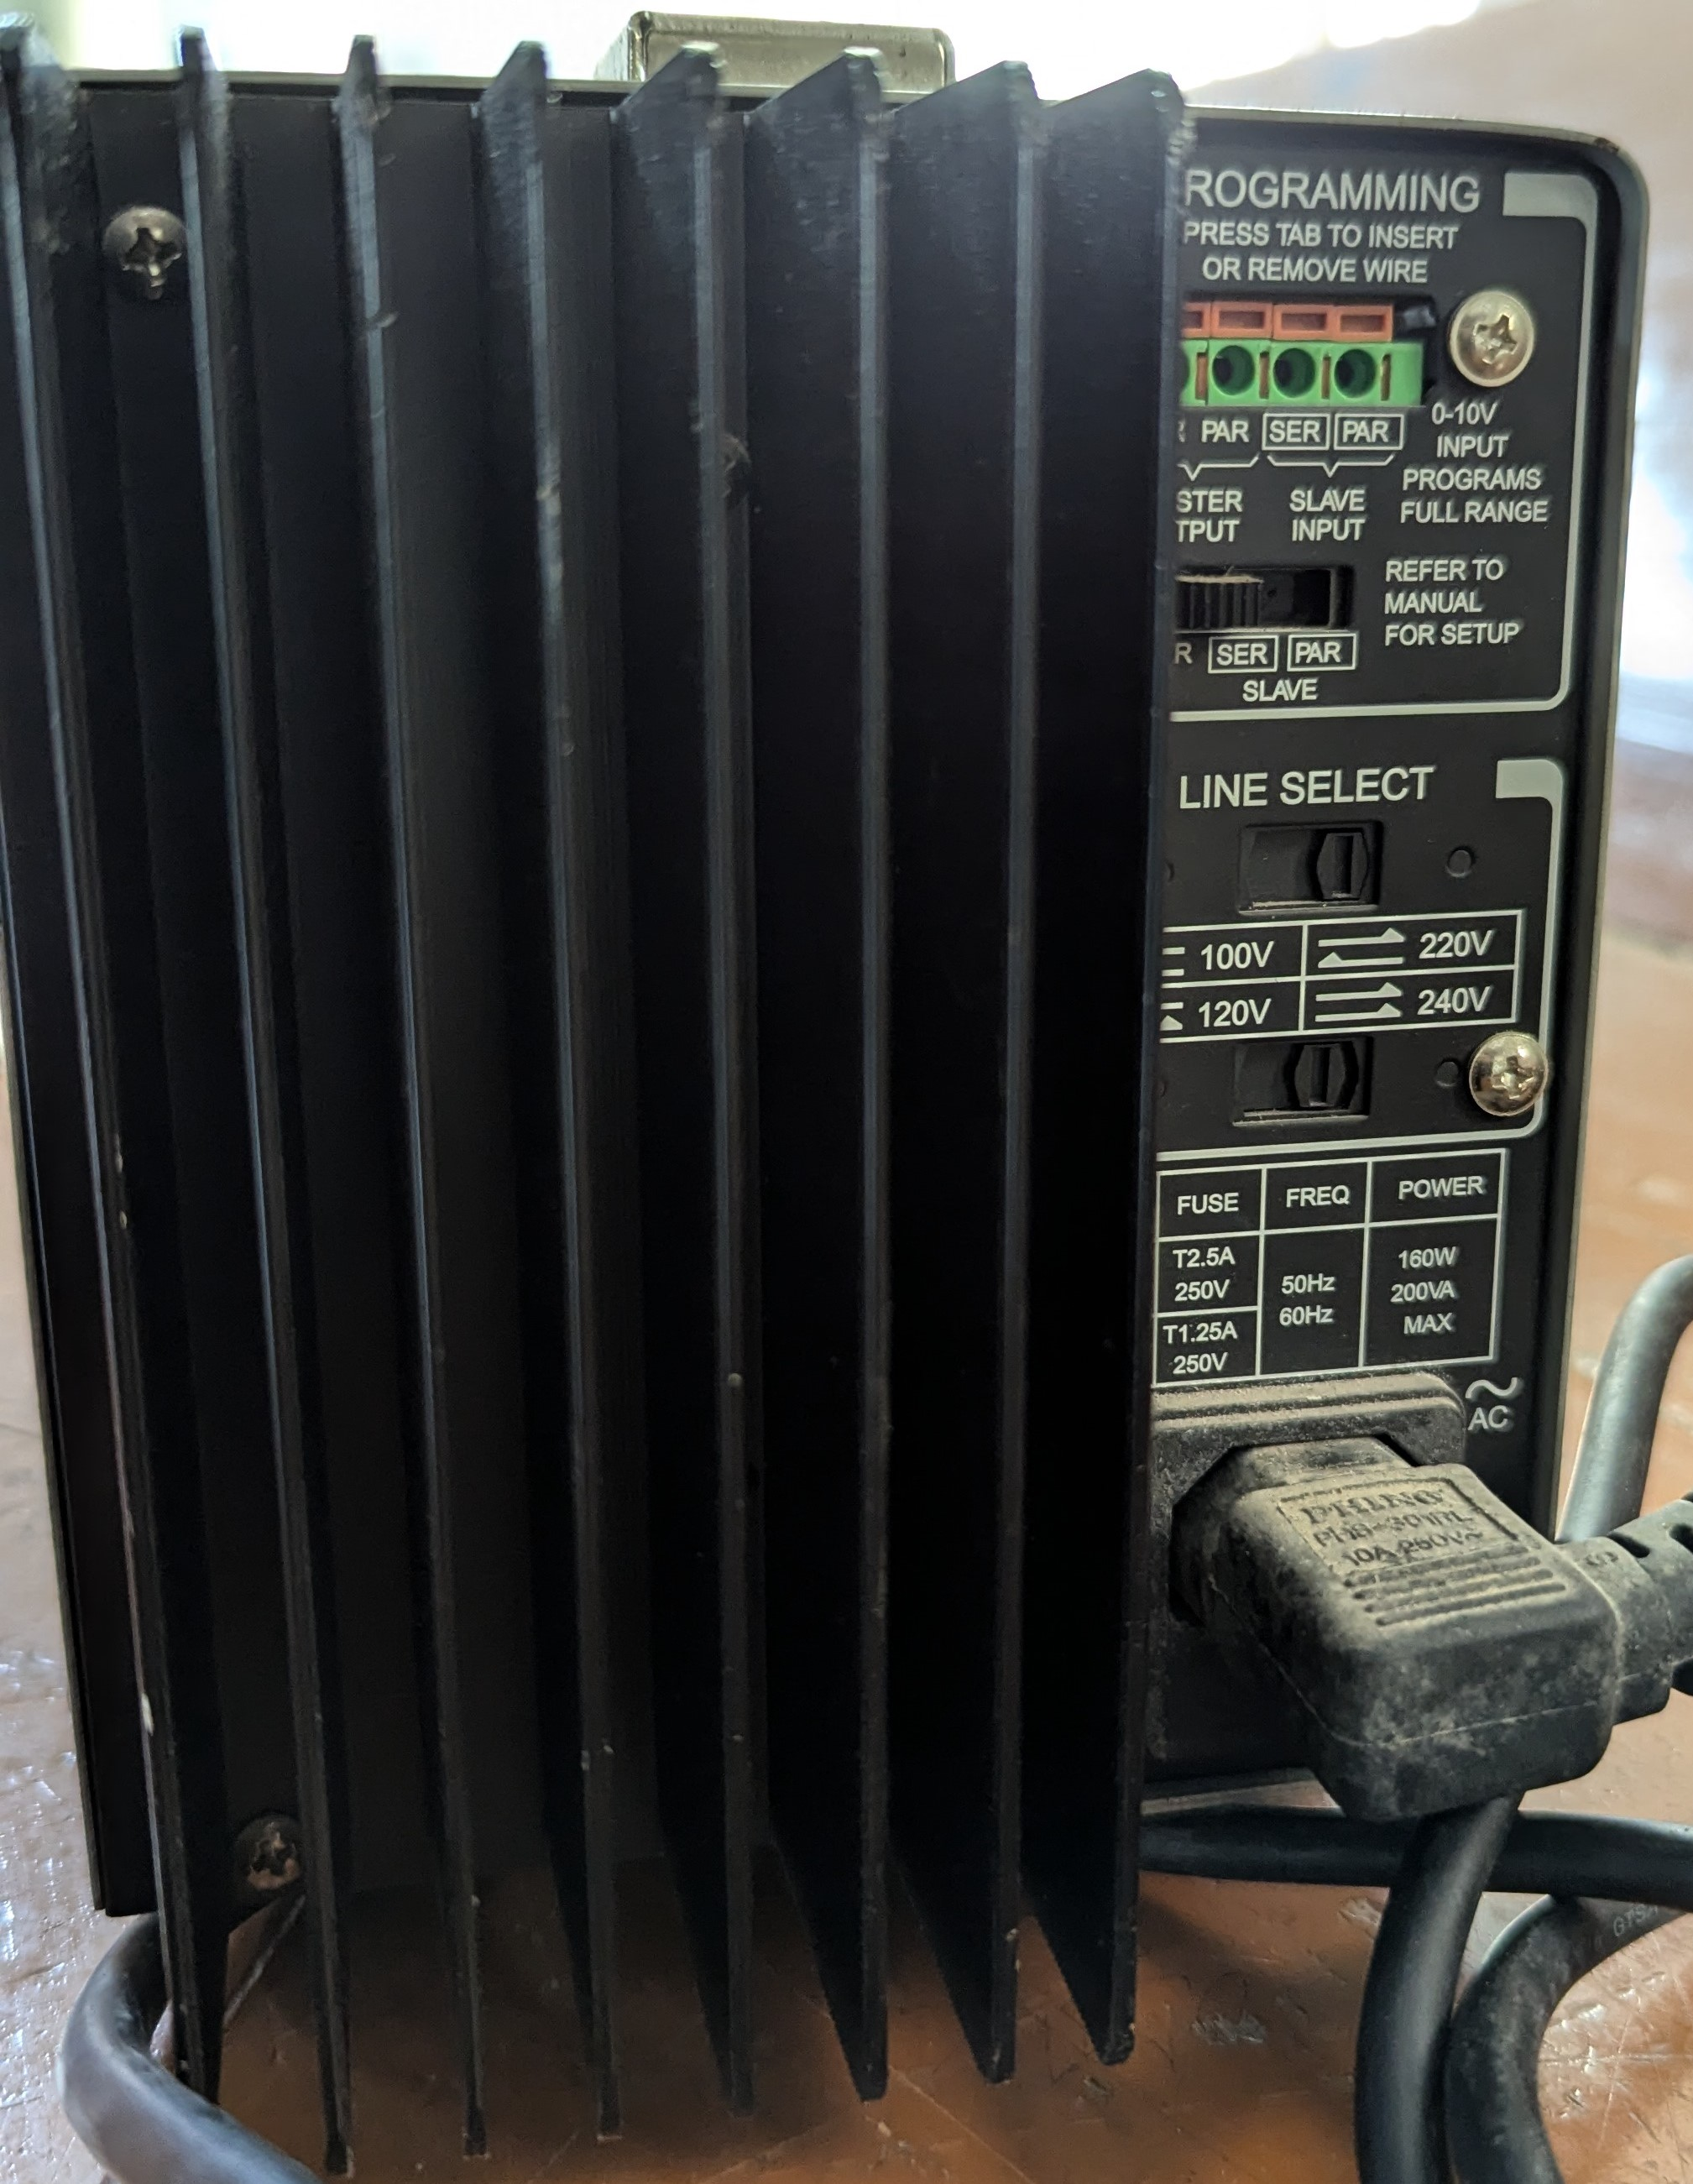
\includegraphics[width=0.8\linewidth]{Images/28}
			\caption{Back View}
		\end{subfigure}}
		
		\caption{Laboratory DC Power Supply}
		\label{fig:5}
	\end{figure}
	
	\section{Discussion}

	
	In the experiment titled \textit{“Introduction to the Available Equipments of Measurement Lab”}, we explored a diverse array of measurement tools essential for electrical engineering tasks. Each instrument, from the voltmeter to the potential transformer, plays a crucial role in measuring and analyzing various electrical parameters. The experiment successfully familiarized us with a broad spectrum of measurement equipment used in the lab, each serving a specific and crucial function in electrical testing and analysis.\\
	By gaining hands-on experience with instruments such as the multimeter, voltmeter, ammeter, and others, we developed a deeper understanding of their operations and applications. The ability to precisely measure voltage, current, and resistance, as well as generate and analyze signals, is essential for accurate experimental results and effective troubleshooting. Mastery of these tools not only enhances practical skills but also prepares us for more advanced experimental setups and analyses. This foundational knowledge is pivotal for future projects and experiments in electrical engineering, ensuring that we can conduct work with confidence and precision.
	
	
\end{document}